% Options for packages loaded elsewhere
\PassOptionsToPackage{unicode}{hyperref}
\PassOptionsToPackage{hyphens}{url}
\PassOptionsToPackage{dvipsnames,svgnames,x11names}{xcolor}
%
\documentclass[
  10pt,
  a4paper,
  numbers=noendperiod,
  DIV=12]{scrartcl}

\usepackage{amsmath,amssymb}
\usepackage{lmodern}
\usepackage{iftex}
\ifPDFTeX
  \usepackage[T1]{fontenc}
  \usepackage[utf8]{inputenc}
  \usepackage{textcomp} % provide euro and other symbols
\else % if luatex or xetex
  \usepackage{unicode-math}
  \defaultfontfeatures{Scale=MatchLowercase}
  \defaultfontfeatures[\rmfamily]{Ligatures=TeX,Scale=1}
\fi
% Use upquote if available, for straight quotes in verbatim environments
\IfFileExists{upquote.sty}{\usepackage{upquote}}{}
\IfFileExists{microtype.sty}{% use microtype if available
  \usepackage[]{microtype}
  \UseMicrotypeSet[protrusion]{basicmath} % disable protrusion for tt fonts
}{}
\makeatletter
\@ifundefined{KOMAClassName}{% if non-KOMA class
  \IfFileExists{parskip.sty}{%
    \usepackage{parskip}
  }{% else
    \setlength{\parindent}{0pt}
    \setlength{\parskip}{6pt plus 2pt minus 1pt}}
}{% if KOMA class
  \KOMAoptions{parskip=half}}
\makeatother
\usepackage{xcolor}
\setlength{\emergencystretch}{3em} % prevent overfull lines
\setcounter{secnumdepth}{3}
% Make \paragraph and \subparagraph free-standing
\ifx\paragraph\undefined\else
  \let\oldparagraph\paragraph
  \renewcommand{\paragraph}[1]{\oldparagraph{#1}\mbox{}}
\fi
\ifx\subparagraph\undefined\else
  \let\oldsubparagraph\subparagraph
  \renewcommand{\subparagraph}[1]{\oldsubparagraph{#1}\mbox{}}
\fi


\providecommand{\tightlist}{%
  \setlength{\itemsep}{0pt}\setlength{\parskip}{0pt}}\usepackage{longtable,booktabs,array}
\usepackage{calc} % for calculating minipage widths
% Correct order of tables after \paragraph or \subparagraph
\usepackage{etoolbox}
\makeatletter
\patchcmd\longtable{\par}{\if@noskipsec\mbox{}\fi\par}{}{}
\makeatother
% Allow footnotes in longtable head/foot
\IfFileExists{footnotehyper.sty}{\usepackage{footnotehyper}}{\usepackage{footnote}}
\makesavenoteenv{longtable}
\usepackage{graphicx}
\makeatletter
\def\maxwidth{\ifdim\Gin@nat@width>\linewidth\linewidth\else\Gin@nat@width\fi}
\def\maxheight{\ifdim\Gin@nat@height>\textheight\textheight\else\Gin@nat@height\fi}
\makeatother
% Scale images if necessary, so that they will not overflow the page
% margins by default, and it is still possible to overwrite the defaults
% using explicit options in \includegraphics[width, height, ...]{}
\setkeys{Gin}{width=\maxwidth,height=\maxheight,keepaspectratio}
% Set default figure placement to htbp
\makeatletter
\def\fps@figure{htbp}
\makeatother
\newlength{\cslhangindent}
\setlength{\cslhangindent}{1.5em}
\newlength{\csllabelwidth}
\setlength{\csllabelwidth}{3em}
\newlength{\cslentryspacingunit} % times entry-spacing
\setlength{\cslentryspacingunit}{\parskip}
\newenvironment{CSLReferences}[2] % #1 hanging-ident, #2 entry spacing
 {% don't indent paragraphs
  \setlength{\parindent}{0pt}
  % turn on hanging indent if param 1 is 1
  \ifodd #1
  \let\oldpar\par
  \def\par{\hangindent=\cslhangindent\oldpar}
  \fi
  % set entry spacing
  \setlength{\parskip}{#2\cslentryspacingunit}
 }%
 {}
\usepackage{calc}
\newcommand{\CSLBlock}[1]{#1\hfill\break}
\newcommand{\CSLLeftMargin}[1]{\parbox[t]{\csllabelwidth}{#1}}
\newcommand{\CSLRightInline}[1]{\parbox[t]{\linewidth - \csllabelwidth}{#1}\break}
\newcommand{\CSLIndent}[1]{\hspace{\cslhangindent}#1}

\usepackage{titlepic}
\usepackage{graphicx}
\usepackage{fancyhdr}
\usepackage{fontspec}
\usepackage{placeins}
\usepackage{graphbox}

\renewcommand{\topfraction}{.9}
\renewcommand{\bottomfraction}{.7}
\renewcommand{\textfraction}{.1}
\renewcommand{\floatpagefraction}{.5}
\renewcommand{\textfloatsep}{14pt}
\setcounter{topnumber}{3}
\setcounter{bottomnumber}{3}
\setcounter{totalnumber}{4}

% \setmainfont{Nunito} [
  %   Extension=.ttf,
  %   UprightFront=*-Regular,
  %   Path = fonts/,
  %   ]

\pagestyle{fancy}
\fancyhf{}
\fancyhead[LO, RE]{MEAPS}
\fancyhead[RO, LE]{
\includegraphics[align=c, width=0.8cm]{ofce.png}}
\fancyfoot[LO, LE]{\small{OFCE}}
\fancyfoot[RE, RO]{\small{\thepage}}
\usepackage{amsmath}
\usepackage{booktabs}
\usepackage{caption}
\usepackage{longtable}
\KOMAoption{captions}{tableheading}
\makeatletter
\makeatother
\makeatletter
\makeatother
\makeatletter
\@ifpackageloaded{caption}{}{\usepackage{caption}}
\AtBeginDocument{%
\ifdefined\contentsname
  \renewcommand*\contentsname{Table des matières}
\else
  \newcommand\contentsname{Table des matières}
\fi
\ifdefined\listfigurename
  \renewcommand*\listfigurename{Figures}
\else
  \newcommand\listfigurename{Figures}
\fi
\ifdefined\listtablename
  \renewcommand*\listtablename{Tableaux}
\else
  \newcommand\listtablename{Tableaux}
\fi
\ifdefined\figurename
  \renewcommand*\figurename{figure}
\else
  \newcommand\figurename{figure}
\fi
\ifdefined\tablename
  \renewcommand*\tablename{tableau}
\else
  \newcommand\tablename{tableau}
\fi
}
\@ifpackageloaded{float}{}{\usepackage{float}}
\floatstyle{ruled}
\@ifundefined{c@chapter}{\newfloat{codelisting}{h}{lop}}{\newfloat{codelisting}{h}{lop}[chapter]}
\floatname{codelisting}{Listing}
\newcommand*\listoflistings{\listof{codelisting}{Liste des Listings}}
\makeatother
\makeatletter
\@ifpackageloaded{caption}{}{\usepackage{caption}}
\@ifpackageloaded{subcaption}{}{\usepackage{subcaption}}
\makeatother
\makeatletter
\@ifpackageloaded{tcolorbox}{}{\usepackage[many]{tcolorbox}}
\makeatother
\makeatletter
\@ifundefined{shadecolor}{\definecolor{shadecolor}{rgb}{.97, .97, .97}}
\makeatother
\makeatletter
\makeatother
\ifLuaTeX
\usepackage[bidi=basic]{babel}
\else
\usepackage[bidi=default]{babel}
\fi
\babelprovide[main,import]{french}
% get rid of language-specific shorthands (see #6817):
\let\LanguageShortHands\languageshorthands
\def\languageshorthands#1{}
\ifLuaTeX
  \usepackage{selnolig}  % disable illegal ligatures
\fi
\IfFileExists{bookmark.sty}{\usepackage{bookmark}}{\usepackage{hyperref}}
\IfFileExists{xurl.sty}{\usepackage{xurl}}{} % add URL line breaks if available
\urlstyle{same} % disable monospaced font for URLs
\hypersetup{
  pdftitle={MEAPS : Distribution statistique des trajets entre le domicile et le travail},
  pdfauthor={Maxime Parodi; Xavier Timbeau},
  pdflang={fr},
  colorlinks=true,
  linkcolor={blue},
  filecolor={Maroon},
  citecolor={Blue},
  urlcolor={Blue},
  pdfcreator={LaTeX via pandoc}}

\title{MEAPS : Distribution statistique des trajets entre le domicile et
le travail\thanks{Nous remercions Francesco Pirri et Pablo Vallier pour
leur travail durant un stage à l'été 2022. Les discussions et les
travaux conduits avec Lucas Pouvrerau, David Miet et Valentin Stuhfault
de Villes Vivantes ont été particulièrement fructueuses. L'application à
la Rochelle a été en partie financée par l'agglomération de la Rochelle
et nous remercions particulièrement Florence Nassiet et Bernard
Habbouche et leurs collègues des services de l'aglomération de la
Rochelle. L'ensemble des calculs a été réalisé sur la plateforme Nuvolos
dont le support technique s'est avéré insdispensable.}}
\usepackage{etoolbox}
\makeatletter
\providecommand{\subtitle}[1]{% add subtitle to \maketitle
  \apptocmd{\@title}{\par {\large #1 \par}}{}{}
}
\makeatother
\subtitle{\emph{version provisoire, ne pas citer, ne pas diffuser}}
\author{Maxime Parodi \and Xavier Timbeau}
\date{03/01/2023}

\begin{document}
\maketitle
\begin{abstract}
Nous proposons un modèle spatial de distribution des trajets entre
emploi et résidence. En s'inspirant du modèle ``intervening
opportunities'' de Stouffer (1940) et du modèle radiatif de Simini et
al. (2012), nous construisons un modèle ergodique d'absorption avec
priorité et saturation (MEAPS) qui permet d'expliciter complètement des
contraintes traitées de façon ad hoc dans la littérature. Le modèle
s'accomode de différentes formulations des processus stochastiques
fondamentaux qui permettent d'en déduire une procédure d'estimation,
tout en conservant un fondement microscopique solide. Une conjecture
d'ergodicité, validée sur des simulations numériques, permet de réduire
les coûts en temps de calcul, autorisant des applications empiriques.
\end{abstract}
\ifdefined\Shaded\renewenvironment{Shaded}{\begin{tcolorbox}[borderline west={3pt}{0pt}{shadecolor}, boxrule=0pt, enhanced, frame hidden, interior hidden, sharp corners, breakable]}{\end{tcolorbox}}\fi

\renewcommand*\contentsname{Table des matières}
{
\hypersetup{linkcolor=}
\setcounter{tocdepth}{1}
\tableofcontents
}
\hypertarget{introduction}{%
\section*{Introduction}\label{introduction}}
\addcontentsline{toc}{section}{Introduction}

Nous nous intéressons à la mobilité de la vie quotidienne et les
facteurs qui la détermine. Pour cela nous voulons à la fois connaître le
nombre de trajets qu'un individu effectue chaque jour ou chaque semaine,
mais aussi quelles sont les destinations probables de ces trajets, les
modes de transport employés et les temps passés à les effectuer. Cette
connaissance suppose une modélisation qui fournit un certain nombre de
prédictions que l'on peut confronter à l'information dont on dispose. En
particulier, on ne dispose pas en général d'une information complète,
même sur un échantillon, des trajets effectués pour chaque individu vers
chacune des destinations possibles, pour chacun des motifs
envisageables. On mesure donc soit des distributions de trajets dans la
population, par motif et par mode, issues d'enquêtes de déplacement soit
des nombre de trajets reliant telle commune de résidence à telle commune
d'activité. L'information, quoique riche, ne couvre pas toute la
complexité du phénomène considéré et la modélisation doit aider à
comprendre et à quantifier le lien entre quelques paramètres
fondamentaux et les observations.

Intuitivement, l'analyse des trajets doit permettre de relier
différentes dimensions de la géographie, de l'endroit où les gens
habitent, à celui où ils s'affairent, en intégrant le réseau de
transport qui leur permet de se déplacer, plus ou moins rapidement, plus
ou moins en sécurité, pour un coût plus ou moins important. Puisque
l'espace est partagé, on s'attend à ce que la congestion ou la densité
des emplois ou des résidences jouent des rôles à un moment ou un autre.
La modélisation doit permettre, autant que possible, d'intégrer ces
couches disparates dans un objet que l'on peut confronter aux données
dont on dispose. Sur la base de cette modélisation, on doit pouvoir
ensuite analyser des changements, que ce soit dans les comportements
individuels, dans les masses d'emplois disponibles ou le nombre
d'habitants, leur répartition spatiale, ou encore dans la structure du
réseau de transport afin de construire des scénarios représentant ce qui
pourrait se passer si (on changeait quelque chose). La confrontation aux
données est alors une étape importante, puisqu'on veut en tirer un
diagnostic sur la modélisation et apprécier le potentiel prédictif.

Pour modéliser les trajets entre des lieux de résidence et des lieux
d'emploi, on procède usuellement par la méthode à 4 étapes (Patrick
Bonnel 2001; Dios Ortúzar et Willumsen 2011). Cette méthode consiste
dans un premier temps à déterminer le nombre de trajets en partance d'un
lieu de résidence ainsi que ceux arrivant au total dans un lieu
d'activité. C'est l'étape 1 de génération des trajets. La seconde étape
consiste à distribuer les trajets de l'étape 1 entre chaque paire de
départ et de destination. C'est l'étape de distribution. La troisième
étape est celle du choix modal, où pour chaque trajet (entre chaque
origine et chaque destination) considéré se voit affecté un mode de
transport. Enfin la quatrième étape du modèle à 4 étapes est celle qui
spécifie le trajet et permet d'en connaître les caractéristiques
précises, comme la distance parcourue, les axes employées ou les
dénivelés effectués. Cette décomposition est un peu arbitraire. Le
nombre de trajets effectué dépend en effet des possibilités ouvertes par
la géographie qui sont définies par les caractéristiques précises des
trajets. L'étape 4 est donc nécessaire pour comprendre l'étape 1, et
l'étape 4 demande de connaître les choix modaux pour être utile aux
choix fait en 1. L'étape 2 est nécessaire pour explorer les possibilités
de trajets. Les imbrications sont nombreuses entre les étapes et la
décomposition n'implique pas l'indépendance.

Nous développons ici un modèle qui permet de distribuer les trajets qui
ont été assignés en première étape. Le modèle gravitaire est employé
généralement dans cette deuxième étape pour prendre en compte le rôle de
la distance. Plus un emploi est loin, moins il doit être attractif. Un
individu doit donc préférer les emplois près de lui à ceux qui sont
éloignés.

Nous discutons dans une première partie des insuffisances du modèle
gravitaire (Section~\ref{sec-grav}), puis nous comparons le modèle
gravitaire à celui de Stouffer (1940) et de Simini et al. (2012) qui
font intervenir le rang de classement des emplois plutôt que la distance
(Section~\ref{sec-rad}). Nous présentons alors une version étendue de ce
modèle ``radiatif'' qui permet deux résultats principaux : 1. au lieu de
la distance, c'est le nombre d'emplois accessibles dans un cercle de
rayon donné qui détermine le choix individuel. 2. nous explicitons la
saturation et nous donnons un fondement microscopique au respect des
contraintes aux marges (tout individu a un emploi, tout emploi est
occupé par un individu) (Section~\ref{sec-meaps}). La formulation est
probabiliste et nous en analysons quelques propriétés par des
simulations synthétiques (Section~\ref{sec-synt}). Nous proposons
ensuite une application à l'agglomération de la Rochelle
(Section~\ref{sec-rochelle}).

\hypertarget{sec-grav}{%
\section{Les insuffisances du modèle gravitaire}\label{sec-grav}}

Le modèle gravitaire est employé très fréquemment en économie spatiale
(Hensher et Button 2007, chap. 2). Il semble en effet répondre de façon
satisfaisante au premier principe de Tobler (Tout est relié mais les
choses proches sont plus reliées que les choses éloignées). Il s'appuie
également sur une analogie avec le modèle de la gravitation dont les
succès en physique et en mécanique sont immenses. Ce modèle est
généralement la pierre angulaire de l'étape de distribution des trajets
dans la décomposition à 4 étapes des modèles de transport (Dios Ortúzar
et Willumsen 2011; Patrick Bonnel 2001, 160). Il est également utilisé
dans d'autres domaines, comme le commerce international ou l'analyse des
épidémies, domaines que nous ne discuterons pas ici.

\hypertarget{les-mauvaises-raisons-du-succuxe8s-du-moduxe8le-gravitaire}{%
\subsection{Les (mauvaises) raisons du succès du modèle
gravitaire}\label{les-mauvaises-raisons-du-succuxe8s-du-moduxe8le-gravitaire}}

Formellement, le modèle gravitaire décrit la force d'une relation entre
deux objets en fonction de leur distance et de leur masse respective.
Par analogie, le modèle gravitaire consiste ici à évaluer le nombre de
trajets professionnels entre deux localisations en prenant pour masses
le nombre d'habitants au point de départ et le nombre d'emplois au point
d'arrivée et, pour distance, une fonction \(f\) croissante de la
distance. On a ainsi, en indiçant les points de départ par \(i\) et les
points d'arrivée par \(j\) :

\begin{equation}\protect\hypertarget{eq-gravity}{}{
T_{i,j} = \frac {N_{hab, i}\times N_{emp, j}} {f(d_{i,j})}
}\label{eq-gravity}\end{equation}

Les premiers modèles gravitaires ont emprunté la fonction \(f\) à la
physique newtonienne (\(f=1/d^2\)), mais d'autres formulations ont
depuis été proposées. Par exemple, la fonction \(f=e^{-d/\delta}\)
intervient dans les modèles de choix discrets proposés par McFadden
(Ben-Akiva et Lerman 2018). En remplaçant la distance par la notion de
coût généralisé du transport, on peut relier cette forme fonctionnelle à
un modèle de choix avec une fonction d'utilité aléatoire (random utility
model). Il est également possible d'ajuster des formes fonctionnelles
plus complexes en ajoutant des paramètres. Le modèle gravitaire arrive
alors à reproduire des distributions de distances observées dans des
enquêtes de transport menées de par le monde. Un raisonnement par
minimisation de l'entropie a été proposé par Wilson (1967) pour donner
un fondement théorique à l'équation~\ref{eq-gravity}. Le raisonnement
est de considérer l'état de référence comme étant celui qui est le plus
fréquent dans une distribution aléatoire des choix. Wilson (1967) montre
alors que, si la fonction \(f\) est donnée, l'équation~\ref{eq-gravity}
a bien la forme proposée et que c'est le produit des habitants et des
emplois qui doit se trouver au numérateur (et non une puissance de l'un
ou l'autre par exemple). Mais rien ne permet de trouver un fondement à
la forme fonctionnelle de \(f\). Le parallèle avec la physique est
simple à faire : l'interaction définit le rôle de la distance, la
maximisation de l'entropie permet d'en déduire que l'équation
macroscopique dépend des masses agrégées, mais ne permet de dire quoique
ce soit de plus sur la nature de l'interaction.

Comme le notent Simini et al. (2012), les fondations théoriques et
empiriques de la fonction \(f\) sont donc faibles. La multiplication des
paramètres pour améliorer l'ajustement n'ont le plus souvent aucune
justification théorique. De fait, on est parfois plus proche d'un
exercice d'interpolation des données que d'un exercice de modélisation
où les paramètres ont une signification explicite. Les comportements
asymptotiques soulignent également des incohérences : par exemple, en
faisant tendre vers l'infini les emplois à l'arrivée, le modèle prédit
un nombre infini de trajets, même si le nombre de résidents au départ
est limité ! Il est également insatisfaisant que le modèle gravitaire
soit déterministe et ne permette ni d'expliquer les fluctuations
statistiques du nombre de trajets prédits, ni d'évaluer la vraisemblance
de différents cas empirique.

Mais la critique la plus forte du modèle gravitaire vient de ses
propriétés fondamentales et des conclusions que l'on peut en tirer. Le
nombre de trajets entre une origine (la résidence) et une destination
(l'emploi) repose sur un simple arbitrage entre distance et quantité de
résidents ou d'emplois. Le comportement du modèle aux limites, à
nouveau, suscite la perplexité : un seul emploi à l'origine devrait être
infiniment préféré un très grand nombre d'emplois un peu plus loin.
C'est tout à fait irréaliste et l'on devine déjà que la distance ne joue
pas un rôle si direct dans les comportements de mobilité. On voit
également que le poids relatif de cet emploi quasi central par rapport
aux ``masses'' d'emplois éloignés va varier de manière irréaliste selon
qu'il est plus ou moins proche de l'origine.

Comme le soulignait déjà Stouffer (1940), ce n'est peut-être pas tant la
distance aux emplois qui est décisive que le rang de ces emplois selon
l'ordre des distances. Dans le modèle gravitaire, il faut faire une
grande différence entre le cas où le deuxième emploi le plus proche est
à 500 m et le cas où il est à 1 km. Si l'on applique le modèle
newtonien, il faudrait croire, par exemple, que l'attractivité de ce
dernier emploi est divisée par 4. Qui peut croire que les 500 m de
différence pèsent d'un si grand poids dans une recherche d'emploi ?
L'attractivité de l'emploi dépend avant tout du fait qu'il s'agit du
deuxième emploi disponible près de chez soi. Empiriquement, il y a peu
de doutes que le modèle gravitaire a de piètres performances : il ne
parvient pas à expliquer pourquoi, lorsque la densité des emplois est
faible autour d'un résident, celui-ci va envisager des trajets plus long
pour atteindre des zones denses en emplois ; c'est pourtant une
observation très commune qui devrait se retrouver dans une modélisation
adéquate.

Assez peu de publications se risquent à une comparaison systématique du
modèle gravitaire avec d'autres formulations qui respecteraient la
première loi de Tobler. On peut citer Heanue et Pyers (1966) comme une
des rares tentatives de ce genre. Le modèle gravitaire semblait moins
bon que le modèle des intervening opportunities (voir plus loin) s'il
n'était pas ajusté de manière ad hoc, comme il est devenu usuel.

Simini et al. (2012) donnent quelques exemples pour les Etats-Unis de la
difficulté du modèle gravitaire à reproduire les comportements
habituels. A l'évidence, le modèle gravitaire ne prédit que des
destinations proches et néglige complètement les destinations
lointaines. Il semble impossible à la forme fonctionnelle \(f(d_{ij})\)
de rendre compte empiriquement à la fois du nombre de trajets courts et
du nombre de trajets distants au travers d'un modèle susceptible de
rendre compte des trajets dans différentes régions, dès lors que les
densités y sont distribuées différemment.

\hypertarget{le-voile-de-la-contrainte-aux-marges}{%
\subsection{Le voile de la contrainte aux
marges}\label{le-voile-de-la-contrainte-aux-marges}}

Le modèle gravitaire peut être complexifié pour mieux coller aux données
qu'il ne le fait spontanément. Il perd alors tout lien avec les
réflexions théoriques le reliant à la maximisation de l'entropie (Wilson
1967) ou au modèle de choix discrets. L'ajustement du modèle devient un
exercice d'interpolation, en s'efforçant de coller autant que possible
aux données, sans plus tester réellement un modèle à l'aide de tests de
vraisemblance. L'exercice consiste ainsi à ajouter une étape de
``normalisation'' au modèle en incorporant dans le modèle des
coefficients correctifs en ligne et en colonne dans la matrice
origine-destination, ce qui revient à ajouter des effets fixes à chacun
des points de départ et d'arrivée. La formulation du modèle gravitaire
est alors modifiée comme suit :

\begin{equation}\protect\hypertarget{eq-gravmod}{}{
T_{i,j} = a_i \times b_j \times \frac {N_{hab, i}\times N_{emp, j}} {f(d_{i,j})}
}\label{eq-gravmod}\end{equation}

La détermination des coefficients \(a_i\) et \(b_j\) pose de nombreux
problèmes. Ces coefficients doivent permettre de respecter les
contraintes aux marges (la somme des emplois pour une ligne de résidents
doit être égale au nombre des résidents employés dans la zone et la
somme des résidents employés sur un lieu d'emploi doit, en colonne donc,
être égale au nombre d'emplois en ce lieu) sur les déplacements. On a
pour \(a_i\) :

\begin{equation}\protect\hypertarget{eq-ai}{}{
a_i = \frac {\Sigma_j T_{i,j}} {\Sigma_j \frac {b_j \times N_{hab, i} \times N_{emp, j}}{f(d_{i,j})}} 
}\label{eq-ai}\end{equation}

\(\Sigma_j T_{i,j}\) est généralement directement observé ou estimé lors
de l'étape de génération dans les approches dites à 4 étapes. C'est le
nombre de départs depuis le point \(i\) et il est proportionnel aux
nombre d'actifs résidant en \(i\). De la même façon on peut écrire pour
\(b_j\) une expression symétrique de celle de \(a_i\), qui fait
intervenir \(\Sigma_i T_{i,j}\) qui est également observée ou estimé
auparavant. C'est le nombre de trajets convergeant vers le point
d'arrivée \(j\), qui est proportionnel au nombre d'emplois en \(j\).

\begin{equation}\protect\hypertarget{eq-bj}{}{
b_j = \frac {\Sigma_i T_{i,j}} {\Sigma_i \frac {a_i \times N_{hab, i} \times N_{emp, j}}{f(d_{i,j})}} 
}\label{eq-bj}\end{equation}

La valeur de \(a_i\), pour un \(i\) donné, dépend de l'évaluation de
tous les \(b_j\) et réciproquement l'évaluation de chaque \(b_j\) dépend
de celle de tous les \(a_i\). On peut estimer ces coefficients par
itérations successives et espérer atteindre de cette manière un point
fixe, éventuellement unique à une constante multiplicative près. Des
algorithmes de résolution ont donc été proposés dans les principaux
manuels (voir par exemple Dios Ortúzar et Willumsen (2011), chapitre 5).
L'application de tels algorithmes (comme celui de Furness, Dios Ortúzar
et Willumsen (2011), p.~192) peut toutefois modifier considérablement le
résultat initial proposé par le modèle gravitaire, au risque d'en trahir
la logique et les justifications initiales. En outre, la multiplicité
des solutions et le choix retenu par l'algorithme demeure un angle mort
de ces méthodes.

Mais surtout, cette procédure itérative se contente de multiplier par
des facteurs arbitraires des lignes et des colonnes de la matrice
origine-destination. Ceci ne change donc pas les poids relatifs des
nombres de déplacements depuis une origine ou vers une destination. Or,
si l'on pense que le modèle gravitaire estime mal ces poids relatifs,
comme nous l'avons affirmé ci-dessus, alors cette normalisation ne
change rien sur le fond : une destination éloignée est si fortement
pénalisée dans le modèle gravitaire qu'aucun facteur multiplicatif ne
peut faire remonter le nombre de trajets vers cette destination, sans
faire crever le plafond au nombre de trajets plus proches. La procédure
de respect des marges aurait pu être formulée différemment, par exemple
en utilisant des corrections additives au lieu de corrections
multiplicatives ou une combinaison d'additivité et de multiplicativité.
Chacune de ces procédures manque toutefois de fondement théorique et, en
toute généralité, peuvent conduire à des équilibres multiples que
l'algorithme de résolution va sélectionner sans que l'on puisse
justifier quoi que ce soit.

Le succès du modèle gravitaire découle en partie de cette ``plasticité''
opérationnelle qui permet de l'appliquer à des observations en
respectant certaines contraintes observées tout en laissant croire qu'un
fondement théorique continue de justifier les opérations. Aussi
l'approche gravitaire est-elle largement reprise dans des modèles
appliquées (notamment les modèles LUTI) en dépit de ses défauts,
peut-être faute de mieux. Mais le décalage avec les données rend urgent
de dépasser cette approche qui ``survit'' en se transformant en boîte
noire.

\hypertarget{sec-rad}{%
\section{Une première alternative : le modèle radiatif}\label{sec-rad}}

Le modèle radiatif est l'une des rares alternatives au modèle gravitaire
(Dios Ortúzar et Willumsen 2011). Il reprend les intuitions de Stouffer
(1940) avec son modèle des ``intervening opportunities'', dont la
logique est la suivante : un migrant prévoit d'aller dans un endroit
distant mais trouve en chemin des opportunités ; il s'interrompt alors
en chemin. Cette distraction de son objectif initial est le résultat des
opportunités rencontrées en chemins, ``intervenantes''. La différence
avec le modèle gravitaire est que ce n'est pas la distance qui détermine
la destination, mais le nombre de rencontres. La distance et la
structure géographique continuent de peser indirectement sur le choix
des destinations puisque plus le migrant parcourt une grande distance,
plus il a de chances de rencontrer des opportunités. La modélisation
initiale de Stouffer souffre toutefois de quelques défauts\footnote{Notamment
  des défauts dans la formalisation qui repose sur une série
  d'approximation pas toujours explicitées et qui rend le modèle peu
  manipulable.} et ne résout pas les questions de capacité ou de respect
des contraintes sur les marges. Mais elle ouvre une autre perspective,
où le rôle de la distance est médiatisé par le nombre d'opportunités
rencontré.

Avec Stouffer, c'est ainsi une autre métrique qui est proposée en lieu
et place de la simple distance spatiale. Elle est liée à la notion
d'accessibilité, c'est-à-dire au nombre d'emplois (et plus généralement
d'opportunités) auxquels à accès un individu pour un temps de trajet ou
une distance maximaux fixés. Un emploi apparaît ainsi d'autant plus
``éloigné'' d'un individu qu'il y a d'emplois plus proches de lui. Le
modèle gravitaire posait que les individus font une grande différence
entre le cas où le deuxième emploi disponible est à 500 m et celui où
cet emploi est à 1 km. Dans la nouvelle perspective, il n'y a pas de
différence car il s'agit toujours du second emploi rencontré. Autrement
dit, la distance est relativisée par la prise en compte du milieu qui
est traversé. Plus le milieu est riche en opportunités, moins il est
nécessaire d'aller loin et, inversement, plus le milieu est désert, plus
il faut accepter d'aller loin.

La proposition de Simini et al. (2012) répond à certaines failles de
Stouffer (1940) en proposant un modèle déduit par analogie avec la
physique qui explicite le processus sous-jacent. L'appellation vient du
modèle radiatif qui décrit l'émission de particules et leur absorption
par le milieu qu'elle traverse. L'intuition est la même que celle de
Stouffer (1940) : tant qu'une particule ne rencontre pas d'obstacle,
elle poursuit son chemin. Elle ne s'arrête qu'en rencontrant un site qui
peut l'absorber. Plus le milieu est dense en obstacles, plus la
particule a des chances de s'arrêter. Dans ce modèle, la distribution
des distances parcourues dépend du milieu et de la quantité de sites
d'absorption rencontrés.

Plus précisément, dans le modèle de radiation, chaque particule est
tirée aléatoirement d'une distribution de probabilité avec une
caractéristique \(z\). Chaque point d'absorption, qui représente un lieu
possible de travail, possède une masse d'emploi \(n_i\) et se voit
attribuer une caractéristique \(z_i\) qui est aléatoire. Les lieux
possibles sont classés par ordre de distance, comme dans le modèle de
Stouffer (1940) et la particule les rencontre dans cet ordre. Le tirage
de \(z_i\) est construit en tirant \(n_i\) fois des \(z\) dans la
distribution de probabilité et en prenant le maximum de ces \(z\). Plus
la masse est grande en \(i\), plus le \(z_{max}\) sera grand. La
particule émise est absorbée si son \(z\) est plus petit que \(z_i\).
Pour représenter que la particule sera émise si elle n'est pas absorbée
par son point de départ, son propre \(z\) est tiré par la même méthode,
c'est-à-dire le maximum de \(m_i\) tirages où \(m_i\) est la masse
d'opportunités en \(i\).

Le résultat principal de Simini et al. (2012) est particulièrement
élégant. La valeur moyenne (notée \(\langle T_{i,j}\rangle\) ) des
trajets partant de \(i\) et allant en \(j\) a une expression qui ne
dépend pas de la distribution de probabilité des \(z\). Elle prend
l'expression suivante, où
\(s_{i,j}=\Sigma_{k \in (i \rightarrow j)^*} n_k\), la somme des
opportunités entre \(i\) (non inclus) et \(j\) (non inclus) :

\begin{equation}\protect\hypertarget{eq-rad}{}{
\langle T_{i,j}\rangle = T_i \times \frac {m_i \times n_j}{(m_i + s_{i,j}) \times (m_i + n_i +s_{i,j})}
}\label{eq-rad}\end{equation}

A partir d'hypothèses générales assez simples, on obtient une
formulation qui s'apparente au modèle gravitaire en remplaçant la
distance par l'accumulation des opportunités entre deux points, dès lors
que les opportunités sont classées dans l'ordre des distances. Cette
formulation respecte autant que le modèle gravitaire le premier principe
de Tobler, mais elle repose sur des hypothèses explicites et permet de
mieux représenter les phénomènes déjà évoqués. Un départ dans une zone
peu dense produira des trajets plus longs pour trouver un nombre
équivalent d'opportunités à des trajets plus courts dans une zone dense.
De plus, aucune étape de ``normalisation'' ad hoc n'est requise et le
modèle est probabiliste, ce qui permet de produire des marges d'erreurs
et des tests empiriques.

Les applications du modèle radiatif à des données diverses (mouvements
pendulaires travail-domicile, appels téléphoniques, migrations,
logistique) produisent des distributions de trajets plus proches des
données que le modèle gravitaire, mettant à mal l'adage selon lequel le
modèle gravitaire serait un ``bon'' modèle, validé par les données.

On notera que le modèle de Simini et al. (2012) admet comme cas limite
le modèle gravitaire. En effet, lorsque la densité d'emplois est
uniforme dans le plan, alors l'accumulation des opportunités est
proportionnelle à la surface et la moyenne de trajets entre \(i\) et
\(j\) est une fonction en \(1/r^4\). Ce cas limite montre sous quelle
condition (très particulière) le modèle gravitaire peut être valide.

Il subsiste deux défauts au modèle radiatif de Simini et al. (2012). Le
premier est le pendant de son élégance : il n'y a pas de paramètres pour
l'ajuster, ce qui limite les capacités du modèle à rendre compte de la
richesses des données. Si l'on veut un modèle de base simple et clair
sur le plan conceptuel, on veut aussi pouvoir enrichir le modèle avec
des paramètres qui auraient du sens. Or la seule proposition qu'ils font
dans ce sens, en introduisant un \(\varepsilon\) pour modifier le poids
du point de départ dans le choix des trajets n'y répond que très
partiellement.

Le second défaut est que le modèle ne traite pas le respect des
contraintes aux marges, en particulier en colonne. Dans
l'équation~\ref{eq-rad} le terme \(T_i\) représente le nombre de départs
de \(i\). Il joue le rôle des coefficients \(a_i\) dans le modèle
gravitaire sous une forme multiplicative simple. Son interprétation est
directe et simple. En revanche, il n'existe pas de pendant aux
coefficients \(b_j\) et il n'est donc pas possible au modèle de tenir
compte d'une contrainte capacitaire : un nombre de particules supérieur
au nombre d'emplois peuvent être absorbées en \(j\).

\hypertarget{sec-meaps}{%
\section{Un modèle ergodique d'absorption avec priorité et saturation
(MEAPS)}\label{sec-meaps}}

Nous proposons maintenant une version étendue et remaniée de l'approche
de Stouffer (1940) qui répond aux critiques que nous faisons au modèle
de Simini et al. (2012). Dans cette section, nous présentons le modèle
dans sa forme plus simple avant d'en exposer les extensions les plus
directes. Des simulations synthétiques permettent alors d'apprécier les
grandes lignes du fonctionnement de ce modèle. Nous discutons ensuite
des procédures d'estimation envisageables ainsi que du développement de
mesures issues de ce modèle.

\hypertarget{rang-choix-des-destinations-et-absorption}{%
\subsection{Rang, choix des destinations et
absorption}\label{rang-choix-des-destinations-et-absorption}}

On considère \(I\) individus et \(J\) emplois\footnote{Dans ce qui suit
  on regarde la relation entre résident et emploi ce qui suggère les
  mobilités domicile travail. C'est principalement pour fixer les idées,
  mais la relation entre résident et tout type d'aménités peut être
  abordée de la même façon. Il est également possible de décliner les
  résident selon des caractéristiques observables et d'indexer le modèle
  par ces catégories.} localisés sur un territoire. Ces localisations
sont fixes et exogènes, ce qui signifie que l'on ne s'intéresse pas au
problème de choix de localisation. Non que ce choix ne soit pas
important, mais nous nous intéressons à la distribution des trajets, une
fois fixées les localisations. L'idée est que pour déterminer le choix
de localisation, il faudra prendre en compte ce que la distribution des
trajets, leur longueur ou le coût généralisé qui leur est associé, nous
apprend.

On suppose que toutes les localisations sont séparées et qu'il n'y a
donc qu'un individu ou qu'un emploi par localisation (les emplois et les
individus peuvent être au même endroit, ça ne change rien). Chaque
individu \(i\) classe par ordre de distance croissante les \(J\) emplois
et les examine dans cet ordre. Il a à chaque fois une probabilité
\(p_a\) de prendre l'emploi. Tant qu'il n'est pas pris, il continue sa
recherche en passant à l'emploi suivant le plus proche (de son point de
départ). La probabilité d'occuper l'emploi \(j\) est donc égale à la
probabilité de ne pas occuper les emplois plus proches multipliée par la
probabilité \(p_a\) d'occuper le poste \(j\). En notant \(r_{i}(j)\) le
rang de l'emploi \(j\) dans le classement des distances depuis \(i\), on
peut écrire \(\bar F(j)\) la probabilité de dépasser le \(jème\) élément
:

\begin{equation}\protect\hypertarget{eq-fbar}{}{
\bar F(j)=(1-p_a)^{r_i(j)}
}\label{eq-fbar}\end{equation}

On définit également la probabilité de fuite de la zone considérée.
Cette probabilité est celle qu'un individu ne trouve pas parmi les \(J\)
emplois celui qui lui convient et donc qu'il renonce ou cherche plus
loin. En supposant pour le moment que cette probabilité est la même pour
tous les individus, \(p_f\), on peut déterminer \(p_a\) :

\begin{equation}\protect\hypertarget{eq-pa}{}{
p_a = 1-(p_f)^{1/J}
}\label{eq-pa}\end{equation}

La probabilité \(P_i(j)\) de \(i\) de s'arrêter en \(j\) est :

\begin{equation}\protect\hypertarget{eq-pij}{}{
P_i(j) = (1-p_a)^{r_i(j)-1} \times p_a = {p_f}^{\frac {r_i(j)-1} {J}} \times (1-{p_f}^{1/J})
}\label{eq-pij}\end{equation}

Cette expression définit donc la probabilité pour un individu \(i\)
d'occuper l'emploi \(j\) comme une fonction de la probabilité de fuite,
le rang de l'emploi et le nombre total d'emploi. La rang de \(j\) n'est
autre que le nombre d'opportunités cumulées du point de départ de \(i\)
jusqu'à \(j\) et remplace la distance, comme dans les expressions de
Stouffer (1940) ou de Simini et al. (2012). Ce nombre n'est autre que
l'accessibilité aux emplois de l'individu \(i\) dans un cercle de rayon
\([ij]\).

Chaque emploi a été supposé distinct spatialement des autres. Dans le
cas où les emplois ne seraient pas séparés et pourraient s'accumuler en
un point ou au sein d'un carreau, la formalisation ne change pas.

La probabilité que l'on s'arrête dans le carreau \(c_d\) situé à une
distance \(d\) de \(i\) où se trouvent \(k\) emplois se déduit de
l'équation~\ref{eq-fbar} puisque les \(k\) emplois ont des rangs
successifs. En notant \(s_i(d)=\sum _{j/d_{i,j}<d}1\) le cumul de tous
les emplois qui sont à une distance strictement inférieure à celle du
carreau considéré pour \(i\) (et donc à l'exclusion des \(k\) emplois du
le carreau \(c_d\)), on a :

\begin{equation}\protect\hypertarget{eq-picd}{}{
P_i(i\in c_d) = {p_f}^{s_i(d)/J}\times(1-{p_f}^{ k/J})
}\label{eq-picd}\end{equation}

En prenant un développement limité au 1\textsuperscript{er} ordre de
cette expression (sous l'hypothèse que \(k\) est petit devant le nombre
total d'opportunités \(J\)) , on obtient, en notant
\(\mu=\frac{-log(p_f)}{J}\) :

\begin{equation}\protect\hypertarget{eq-picddl}{}{
P_i(i\in c_d) \approx k\times \mu \times e^{-\mu \times s_i(d)}
}\label{eq-picddl}\end{equation}

Cette expression fait apparaître clairement le cœur du modèle. La
proportion d'emplois venant de \(i\) dans le carreau est une fonction
des emplois dans le carreau multiplié par l'accessibilité jusqu'à ce
carreau de \(i\).

Lorsque la densité des emplois est constante sur un plan, \(s_i(d)\) est
proportionnel à la surface et le modèle devient une fonction de la
distance avec un terme en \(e^{-r^2/\rho^2}\). Ici aussi, le
comportement de notre modèle rejoint, sous cette condition très
particulière d'une répartition homogène des opportunités, celui proposé
pour un modèle gravitaire, lorsque celui-ci est spécifié avec une
fonction de distance en \(e^{-r/\rho}\). La forme favorite du modèle
gravitaire se justifierait pour une répartition homogène des
opportunités le long d'une droite\footnote{La littérature sur le
  commerce international fait un grand usage du modèle gravitaire et on
  y trouve des développements très riches. Le problème du commerce
  international est un peu différent de celui de l'analyse des
  distribution de déplacement parce qu'on observe les flux bilatéraux
  par produit de façon répétée entre les pays. On dispose ainsi d'une
  grande quantité d'informations à relier entre elles par la
  représentation gravitaire. La question du transport est différente en
  ce que la distance entre origines et destination est bien connue, mais
  que les trajets bilatéraux ne le sont pas. On dispose en revanche
  d'information sur la distribution des trajets en fonction de leur
  distance, de leur motif et des modes employés.}. Ce résultat diffère
de celui de Simini et al. (2012), qui trouvaient un comportement
asymptotique en \(1/r^4\).

Tout comme dans le modèle de Simini et al. (2012), le résultat est sans
paramètre, parce que la probabilité de fuite est entièrement déterminée
par la contrainte en ligne (l'individu \(i\) a une espérance égale à 1 -
\(p_f\) de trouver un emploi dans la zone considérée).

\hypertarget{sec-priorite}{%
\subsection{Saturation et priorité}\label{sec-priorite}}

Il reste encore à prendre en compte la contrainte en colonne,
c'est-à-dire le fait que chaque emploi peut être pourvu une fois et une
seule. Au lieu d'un ajustement ad hoc qui tombe de nulle part, nous
proposons le mécanisme suivant de remplissage des emplois : chaque
individu \(i\) est classé selon un ordre de priorité. L'individu au
premier rang est confronté à l'ensemble des emplois et nous calculons
ses probabilités de prendre un emploi \(j\) par la formule précédente
(équation~\ref{eq-pij}). Les emplois sont alors partiellement remplis à
proportion de ces probabilités\footnote{En toute rigueur, les
  probabilités ne s'additionnent pas si simplement et un traitement
  exact exigerait de tenir compte de probabilités conditionnelles au
  fait que tel emploi a été pris, ou non, auparavant. La procédure
  décrite ici est une simplification, en subsituant aux probabilités
  conditionnelles des espérances.}. Le deuxième individu est traité de
la même manière, et ainsi de suite, jusqu'à ce qu'un ou plusieurs
emplois soient totalement pourvu (lorsque la somme des probabilités
dépasse tout juste 1). On retire alors ces emplois de la liste des choix
possibles et on continue l'affectation pour les individus suivants sur
la liste réduite. A chaque individu ajouté, on peut être amené à retirer
d'autres emplois de la liste de recherche.

A la fin de ce processus, tous les individus ont des emplois (à \(p_f\)
près) et tous les emplois sont pourvus dès lors que l'on pose
\(I \times p_f = J\). Cette attribution avec priorité est
Pareto-optimale. Il n'est pas possible d'augmenter la satisfaction d'un
individu sans dégrader celle d'un autre. A chaque étape, chaque individu
réalise ses choix sans contrainte autre que l'éventuelle saturation
provoquée par ses prédécesseurs. Pour augmenter sa satisfaction,
c'est-à-dire lui permettre d'occuper en probabilité un emploi mieux
classé pour lui, il faudrait dégrader la situation d'un prédécesseur en
lui attribuant un emploi plus éloigné pour lui. Cette procédure
d'affection avantage les premiers du classement, mais tient compte des
choix de chacun.

Formellement, on note \(\phi_u(i,j)\) la probabilité de disponibilité
(\(\phi\) vaut 0 si l'emploi est complètement pris) de l'emploi \(j\)
pour un ordre de priorité donné \(u\) au moment où l'individu \(i\) doit
choisir. La probabilité de cet individu \(i\) de prendre l'emploi \(j\)
s'écrit alors :

\begin{equation}\protect\hypertarget{eq-puij}{}{
P_{u, i}(j) = \lambda_{u,i}.\phi_u(i,j). p_a \prod_{l=1}^{r_i^{-1}(j)-1}(1-\lambda_{u,i}. \phi_u(i,r^{-1}(l)).p_a)
}\label{eq-puij}\end{equation}

Cette expression est rendue complexe par la nécessité de parcourir les
emplois dans l'ordre qui correspond à chaque individu. La probabilité
\(p_a\) doit alors être calculée pour que le taux de fuite de \(i\) soit
inchangé. On suppose que les emplois restants demeurent homogènes tout
au long du processus d'affectation. La probabilité de chacun est donc
identique et ajustée d'un facteur multiplicatif \(\lambda_{u,i}\). Le
terme \(\lambda_{u,i}\) découle ainsi de l'indisponibilité potentielle
des emplois. Lorsqu'un emploi est indisponible, l'individu \(i\),
lorsque c'est son tour de choisir, connait ses cibles potentielles. Il
ajuste donc sa probabilité d'absorption de façon à respecter la
probabilité de fuite. Nous choisissons cette option afin de continuer à
respecter la contrainte en ligne, qui s'exprime par
l'équation~\ref{eq-lambda} ci-dessous. Ceci signifie qu'un individu a
d'autant plus de chances d'accepter un emploi qu'il reste peu de choix.

Une autre solution serait de considérer que la probabilité de fuite
n'est pas conservée et que les indisponibilités se traduisent par une
fuite plus élevée. On peut tout à fait envisager des solutions plus
complexes. Nous nous en tenons pour l'instant au cas simple où tous les
individus ont la même chance de travailler dans la zone
considérée\footnote{En pratique, pour éviter les effets de bord, il faut
  choisir une zone d'emplois plus grande que la zone des résidents.}.
Sous cette hypothèse de conservation de la probabilité de fuite, on a :

\begin{equation}\protect\hypertarget{eq-lambda}{}{
\prod_{j=i} ^{J} (1-\lambda_{u,i} \times \phi_u(i,j) \times p_{a})= p_f
}\label{eq-lambda}\end{equation}

La solution de cette équation est celle d'un polynôme en
\(\lambda_{u,i}\) d'un ordre élevé. Il y a possiblement plusieurs
solutions, mais il est nécessaire que \(0<\lambda_{u,i}\times p_a<1\),
ce qui réduit le nombre de solutions admissibles. On peut en produire
une solution approchée par un développement limité à l'ordre 1 en
prenant le \(log\) de l'équation~\ref{eq-lambda} :

\begin{equation}\protect\hypertarget{eq-lambdadl}{}{
p_{a} \times \lambda_{u,i} = \frac {-log(p_f)}{\sum_{j=1} ^{J} \phi_u(i,j)}
}\label{eq-lambdadl}\end{equation}

On peut vérifier que \(0<\lambda_{u,i}\times p_a<1\) lorsque \(J\) est
assez grand et que le nombre d'emplois restant demeure élevé (en
probabilité) par rapport à \(-log(p_f)\).

\hypertarget{sec-erg}{%
\subsection{Ergodicité}\label{sec-erg}}

Chaque ordre de priorité \(u\) définit une trajectoire possible
d'affectation des emplois aux résidents (ou l'inverse). On aboutit à
chaque fois à un état possible de l'appariement résidents-emplois d'où
l'on déduit les trajets professionnels. Bien entendu, le résultat final
dépend de l'ordre de priorité choisi. Pour s'en affranchir, la stratégie
usuelle en physique statistique consiste à réitérer la procédure pour
tous les ordres possibles de priorité et à considérer la moyenne des
résultats obtenus sur les \(I!\) ordres de priorité possibles.

L'hypothèse ergodique consiste ici à soutenir que cette moyenne sur tous
ces ordres de priorité est proche du régime permanent des trajets
professionnels sur la zone considérée.

La première grandeur que nous moyennons sur les ordres \(u\) est la
variable de disponibilités \(\phi_u(i,j)\) de l'emploi \(j\) pour le
résident \(i\). Cette moyenne \(\langle\phi\rangle_u(n,j)\) correspond à
la probabilité de disponibilité de l'emploi \(j\) pour n'importe quel
résident après que \(n\) résidents occupent d'ores et déjà un emploi ou
ont fuit la zone. Cette grandeur ne dépend pas de \(i\), mais uniquement
du nombre de résidents déjà positionnés.

Un deuxième grandeur nous sera utile. Il s'agit de l'accessibilité
moyenne aux emplois disponibles. On peut noter \(A_u(i,k)\) le cumul des
emplois qui restent disponibles pour \(i\) lorsque \(n\) résidents se
sont d'ores et déjà positionnés, en comptant les emplois depuis le plus
proche de \(i\) jusqu'au \(k^{ième}\) le plus proche. La grandeur qui
nous intéresse est la moyenne sur tous les \(n\) possibles, soit :

\begin{equation}\protect\hypertarget{eq-an}{}{
\langle A \rangle_n(i,k) = \langle\sum_{l=1}^k \langle \phi \rangle_u(n, r_i(k)) \rangle _n
}\label{eq-an}\end{equation}

La particularité de cette accessibilité est qu'à mesure que les emplois
sont pris (lorsque \(n\) s'accroît), l'accessibilité se restreint
puisqu'elle ne retient que la part encore disponible des emplois
proches.

Comme précédemment, nous considérons que la probabilité de fuite d'un
individu est une constante. Dans ce cas, la probabilité d'absorption va
augmenter au fur et à mesure que les emplois sont pris : moins il reste
d'emplois disponibles, plus un résident est prêt à accepter ceux qui
restent. La probabilité \(P_a\) va donc dépendre de \(n\) et s'écrire
ici \(P_{a,n}\).

Pour un \(n\) donné, on a :

\begin{equation}\protect\hypertarget{eq-pf2}{}{
P_f=\prod_{k=1}^J(1-P_{a,n}\times \langle \phi \rangle_u(n, r_i(k))
}\label{eq-pf2}\end{equation}

En passant en \(log\) et en effectuant un développement limité, on
obtient :

\begin{equation}\protect\hypertarget{eq-logpf}{}{
log(P_f)=-P_{a,n}\times\sum_{k=1}^J \langle \phi \rangle_u(n,r_i(k))=-P_{a,n}\times(J-(1-P_f)\times n)
}\label{eq-logpf}\end{equation}

Nous avons alors tous les éléments pour calculer la probabilité
\(P_n(i,j)\) que le résident \(i\) prenne l'emploi \(j\) après que \(n\)
résidents se sont déjà positionnés (cf. équation~\ref{eq-pij}). En
passant alors en \(log\), on a :

\begin{equation}\protect\hypertarget{eq-logpij}{}{
log(P_{ij})=log(P_{a,n})+log(\langle\phi \rangle_u(n,j))+\sum_{k=1}^{r_i^{-1}(j)}log(1-P_{a,n}\times \langle \phi \rangle_u(n,r_i(k))
}\label{eq-logpij}\end{equation}

En faisant un développement limité du dernier terme puis la moyenne sur
les \(n\), il en découle :

\begin{equation}\protect\hypertarget{eq-logpijapprox}{}{
log(P_{ij})\approx\langle log(P_{a,n})\rangle _n+\langle\langle\phi\rangle_u(n,j)\rangle_n + \langle A\rangle_n(i, r_i^{-1}(j))
}\label{eq-logpijapprox}\end{equation}

La probabilité \(P_{ij}\) s'écrit donc à partir de la probabilité
moyenne d'absorption, de l'espérance que l'emploi \(j\) est disponible
et de l'accessibilité moyenne. Sur le plan conceptuel, c'est tout à fait
satisfaisant et compréhensible.

\hypertarget{sec-hetero}{%
\subsection{Hétérogénéité de la fuite et de
l'absorption}\label{sec-hetero}}

Nous avons considéré jusqu'à présent le cas où les individus et les
emplois étaient homogènes et indiscernables. Cela simplifie le modèle et
permet une résolution explicite. Il est cependant possible de
complexifier le modèle en levant ces hypothèses en introduisant des
paramètres interprétables qui permettent une meilleure prédiction et
l'extraction d'informations des données.

Tout d'abord, le paramètre de fuite peut être spécifique à chaque
individu. Par exemple, le recensement nous permet de mesurer la
proportion d'individu, par commune, qui ont un emploi à plus de 100km de
leur domicile. Cette proportion est faible (\(<5\%\) pour une région
comme celle étudiée dans l'application à la Rochelle
Section~\ref{sec-rochelle}) mais peut varier d'une commune à l'autre.
Ces variations peuvent s'expliquer par une géographie particulière ou
par des caractéristiques des individus. On peut alors définir une
probabilité de fuite \(p_{f,i}\) pour chaque individu.

Ensuite, le paramètre d'absorption était jusqu'à maintenant identique
pour tous les emplois et tous les individus. On peut le rendre dépendant
des emplois, \(p_{a,j}\), pour marquer un effet fixe spécifique à des
emplois. Le recensement nous donne quelques informations sur les trajets
professionnels de commune à commune et, donc, sur l'attractivité
différentielle entre communes. D'autres données pourraient nous informer
à un niveau infra-communal. On pourrait aussi vouloir faire dépendre la
probabilité d'absorption de caractéristiques observables des emplois.
Des emplois dans une zone dense en emploi peuvent, au-delà de l'effet
masse déjà pris en compte, être plus attractifs que des emplois isolés.
Dans ce cas, l'absorption dépend de caractéristiques \(X\) observées et
en spécifiant la forme fonctionnelle de \(p_a(X)\) on peut l'estimer de
façon à mieux reproduire l'information sur la distribution des
déplacements.

Le modèle présenté est suffisamment flexible pour pouvoir rendre compte
de phénomènes plus complexes afin de, à la fois, pouvoir exploiter des
données riches et modéliser des comportements (de fuite, d'absorption)
qui semblent avoir un sens. Si au lieu d'apparier les individus et les
emplois, on s'intéresse au cas du choix des écoles, on peut imaginer que
l'absorption de l'école la plus proche est élevée, mais que celles de
rang supérieur s'effondrent. Si l'individu est indifférent aux
caractéristiques des écoles, hors leur emplacement, il prend l'école la
plus proche. Le refus de cette première école peut s'expliquer par une
exigence parentale non observable, mais qui se traduit par une distance
parcourue plus élevée. Mais le modèle de base rendant compte d'une
baisse de l'absorption au-delà du premier rang est déjà assez
bon\footnote{De façon plus générale, on peut spécifier une loi de la
  probabilité d'absorption quelconque qui doit vérifier que
  \(\sum_{k=1,J} p_{i,r_i(k)} = p_{f,i}\) pour tout \(i\). Toute
  paramétrisation de cette loi de probabilité peut alors être simulée et
  ajustée sur des données. Si les paramètres ont une interprétation
  théorique, on peut alors les identifier.}.

On peut ainsi modifier les probabilités d'absorption en donnant à un
groupe particulier de paires individus emplois plus ou moins de chances
d'être absorbé. En jouant sur les groupes qui partionnent les paires
individus \(\times\) emplois on peut augmenter ou réduire le nombre de
degré de liberté du système. Lorsque seule la probabilité d'absorption
est un paramètre, le nombre de dégré de liberté est 1 et le paramètre
\(p\) est déterminé par la condition d'égalité entre le nombre d'emplois
pourvus et d'individus. Si on dispose d'une information sur la
probabilité de fuite par indidividu ou par groupe d'individus, le nombre
de degré de liberté peut être accru par une probabilité de fuite
différenciée selon ces groupes. On peut encore accroître le nombre de
degré de liberté en croisant une probabilité d'absorption par groupes
d'emplois et groupes d'individus. Le choix de la spécification dépendra
de ce que l'on souhaite réaliser et du problème considéré. On verra dans
la Section~\ref{sec-rochelle} une application en recourant à un grand
nombre de degré de liberté afin d'ajuster le modèle sur des données
détaillées (donnant pour des paires commune de résidence \(\times\)
commune d'emploi une observation des flux de mobilité professionnels) et
de pouv oir procéder à des intrapolations, en projetant les flux à une
échelle infra communale tout en respectant les observations, et de
pouvoir simuler des scénarios alternatifs en considérant que les
\(\lambda_{i,j}\) sont constants. Dans une publication ultérieure, nous
montrerons une détermination parcimonieuse des coefficients correcteurs
afin de pouvoir extraire une information pertinente des données de flux
entre communes et de pouvoir comparer le pouvoir prédictif de MEAPS à
celui d'un modèle gravitaire, à degré de liberté égal.

En indexant par \(i\) les probabilités de fuite \(p_{f,i}\) et par
\(i,j\) les coefficients correcteurs \(\lambda_{i,j}\), les équations
principales du modèle deviennent :

\begin{equation}\protect\hypertarget{eq-comp1}{}{
P_{i, u}(j) = \lambda_{i,j} . p_{a} \prod _{l=1} ^{r_{u(i)}(j)-1} {[1-\lambda_{i,r_{u(i)}(l)}. p_{a}.\phi_u(i,r_{u(i)}^{-1}(l))]}
}\label{eq-comp1}\end{equation}

\begin{equation}\protect\hypertarget{eq-lambdacomp}{}{
\prod _{l=1} ^{J} {[1-\lambda_{i,r_{u(i)}(l)}.p_{a}.\phi_u(i,r_{u(i)}^{-1}(l))]}= p_{f,i}
}\label{eq-lambdacomp}\end{equation}

Il n'est pas possible de donner une forme réduite de cette dernière
expression. En revanche, elle est calculable numériquement pour chaque
\(u\), \(i\) et \(j\) en fonction des hypothèses du modèle (\(p_{f,i}\),
\(p_{a,j}\), la structure spatiale des résidents et des emplois) et sert
de base à l'algorithme de calcul employé dans les simulations présentées
dans la section Section~\ref{sec-synt}\footnote{L'implémentation de
  cette expression est faite dans le fichier \texttt{meaps.cpp}
  accessible sur le dépôt \texttt{github.com/xtimbeau/meaps}}.

Le modèle ainsi construit est flexible puisqu'on peut spécifier des
processus de fuite (contrainte en ligne équivalente à la contrainte
\ref{eq-ai}) et des processus d'absorption qui respecte la contrainte de
saturation des emplois (contrainte en ligne équivalente à la contrainte
\ref{eq-bj}) par le processus de priorité décrit en
Section~\ref{sec-priorite}. Le parcours de toutes les permutations
possibles permet de s'affranchir d'un ordre de priorité particulier et
de définir une solution moyenne au processus. Lorsqu'on analyse le
problème avec une grille de taille finie (ou de taille inférieure au
nombre \(J\) d'opportunités), on peut conjecturer un comportement
ergodique des quantités moyennes prédites par le modèle. On résout de
cette façon explicitement le problème de contrainte aux marges du modèle
gravitaire ou du modèle radiatif.

\hypertarget{synthuxe8se-de-meaps}{%
\subsection{Synthèse de MEAPS}\label{synthuxe8se-de-meaps}}

Avant de passer aux simulations, résumons le propos : nous proposons une
formulation du problème de distribution des transports qui permet de
traiter du respect de la contrainte aux marges avec un processus
élémentaire explicite. Cela accroît la validité du modèle et sa possible
utilisation dans des applications. Cela permet également d'utiliser
l'information donnée par les contraintes de marge et d'en déduire une
série d'indicateurs caractérisant la zone étudiée et les tensions entre
l'offre et la demande.

La formulation la plus simple du modèle, correspondant à l'hypothèse
d'homogénéité des emplois, d'un processus binaire d'absorption et d'une
valeur identique de fuite par individu permet de construire une
calibration canonique, qui ne dépend que des paramètres de ``masse'' et
de ``distance''. On peut alors proposer une version plus riche du
modèle, en individualisant la probabilité de fuite, en pondérant les
probabilités d'absorption ou encore en proposant un processus
d'absorption non binaire et paramétrique. Ces versions peuvent alors
être confrontées aux données disponibles, en contrôlant du risque de sur
ajustement et en disposant pour chacun des paramètres d'une une
référence canonique.

Comme il est d'usage de le discuter en économie, cette approche est
structurelle et donne aux paramètres un statut exogène. L'identification
sur les données, conditionnellement à ce modèle, peut alors recevoir une
interprétation causale.

\hypertarget{sec-synt}{%
\section{Simulations numériques synthétiques}\label{sec-synt}}

Pour étudier quelques unes des propriétés du modèle nous proposons ici
d'explorer son comportement sur des données synthétiques. Les données
synthétiques, générées de façon explicites, permettent de contrôler les
variations de paramètres afin d'en isoler les conséquences. Ces
simulations ne prétendent pas ni à l'exhaustivité ni à la démonstration,
mais peuvent servir à appuyer l'intuition. L'ensemble de la partie sur
les simulations synthétiques est exécutable au sens de (Lasser 2020).
Les codes nécessaires à la reproduction de ces simulations et des
graphiques associés sont disponibles sur
\texttt{github.com/xtimbeau/meaps} et exécutables librement.

\hypertarget{trois-puxf4les-en-centre-et-satellites}{%
\subsection{Trois pôles en centre et
satellites}\label{trois-puxf4les-en-centre-et-satellites}}

Nous construisons un territoire abstrait composé d'un ``centre ville''
et de ``deux périphéries'' (figure~\ref{fig-territoire}). Cette
configuration arbitraire nous permet d'évaluer MEAPS en simulant les
trajets et leur distribution. Chaque individu et chaque emploi sont
localisés, distinctement les uns des autres, ce qui permet de calculer
des distances euclidiennes entre chaque habitant et chaque emploi et
d'en déduire un classement pour chaque habitant sans ambiguïté des
emplois en fonction de leur éloignement de chaque résident. Tous les
emplois sont considérés comme homogènes et on suppose une probabilité de
fuite identique de 10\% pour tous les individus. Les distances entre les
pôles sont données dans le tableau~\ref{tbl-distances} (dans une unité
sans intérêt).

\hypertarget{tbl-distances}{}
\begin{longtable}{lrrr}
\caption{\label{tbl-distances}Distances entre les pôles }\tabularnewline

\toprule
 & e1 & e2 & e3 \\ 
\midrule
h1 & $0.0$ & $0.6$ & $0.7$ \\ 
h2 & $0.6$ & $0.0$ & $1.3$ \\ 
h3 & $0.7$ & $1.3$ & $0.0$ \\ 
\bottomrule
\end{longtable}

Pour assurer l'égalité entre demandes et offres d'emploi, on tire
aléatoirement 4 500 emplois. Les trois pôles d'emplois ont les mêmes
centres que les pôles d'habitation, mais ont une répartition plus
resserrée que pour les habitants. Comme indiqué sur la
figure~\ref{fig-territoire}, les tâches d'emplois 1 à 3 sont
respectivement localisés autour des mêmes centres que les zones
d'habitation 1 à 3.. Les pôles périphériques comportent moins d'emplois
(5\% chacun) que le pôle central (80\% de l'emploi total) afin de
représenter dans les pôles périphériques des emplois présentiels, liés
aux services fournis aux résidents (comme des commerces ou des écoles)
et d'une zone d'activité centrale. Nous ne faisons aucune distinction de
productivité ou de qualification nécessaire pour les emplois. Cette
hypothèse simplifie la simulation du modèle, mais rien n'empêche de
distinguer des catégories d'emplois, des catégories d'habitants ni
d'introduire des éléments de choix entre distance et nature de l'emploi.
Nous ne considérons ici pas le choix de la localisation et considérons
toutes les localisations comme exogènes.

Dans l'analyse statistique qui suit, on procédera à une agrégation
spatiale en pavant le plan où sont localisés emplois et habitants par
des hexagones adjacents. Cela correspond à une analyse empirique où les
données de localisation sont carroyées.

\begin{figure}[htb]

{\centering 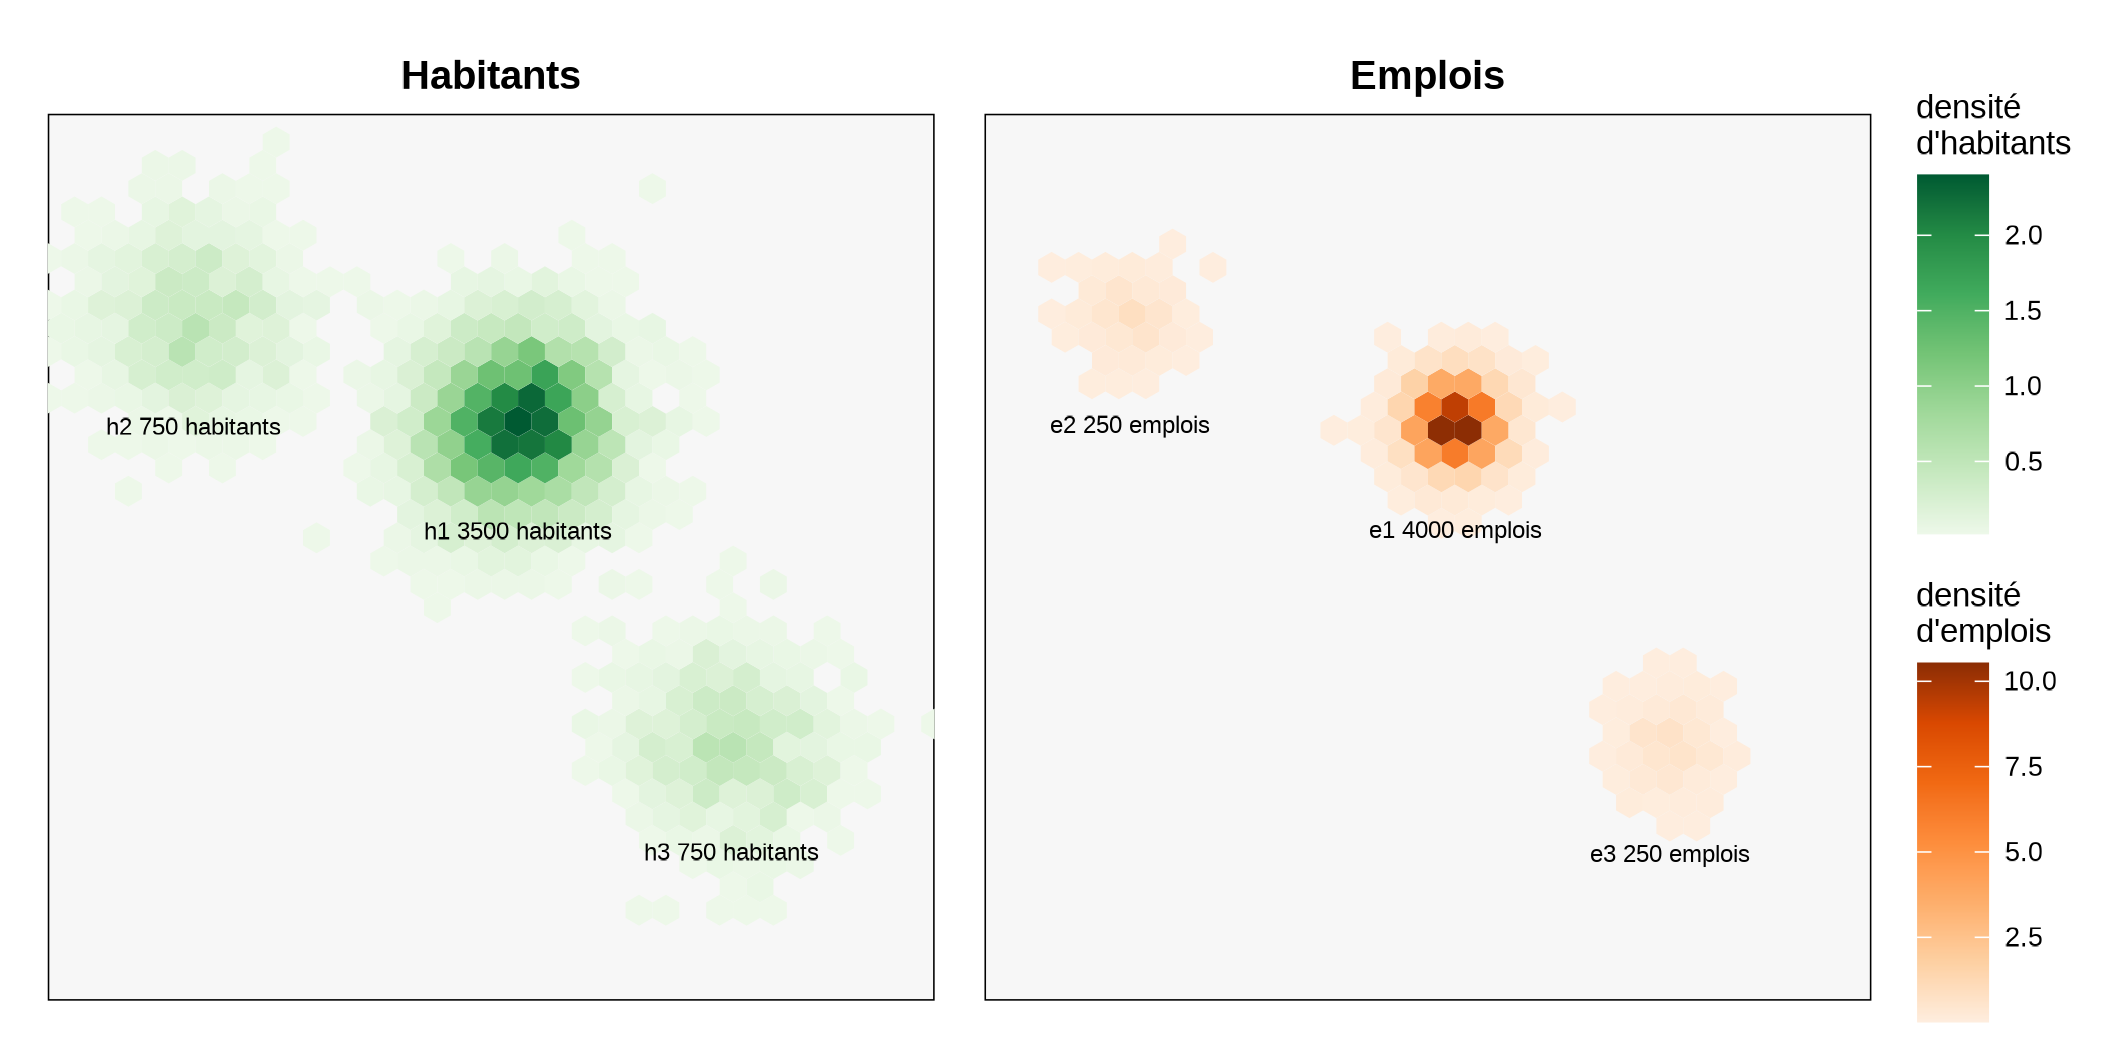
\includegraphics[width=1\textwidth,height=\textheight]{svg/gcarte_ss.png}

}

\caption[Territoire synthétique (centre + 2
villages)]{\label{fig-territoire}Territoire synthétique comportant un
centre ville (h1) et deux villages (h2) et (h3). Dans chaque hexagone
est indiqué la densité (5 000 habitants). 4 500 emplois avec des
proportions d'emplois de 80\% dans le centre et de 5\% dans les 2
villages (les 10\% restant sont la fuite). La dispersion est plus basse
pour les emplois. Les densités d'emplois sont représentées dans le
panneau de droite en orange.}

\end{figure}

La figure~\ref{fig-distances} simule MEAPS à partir des données de
figure~\ref{fig-territoire}. On obtient pour chaque hexagone où résident
des habitants une valeur moyenne de distance jusqu'à leur emploi. De la
même façon, on calcule pour chaque emploi la distance accomplie en
moyenne pour l'atteindre.

\begin{figure}[htb]

{\centering 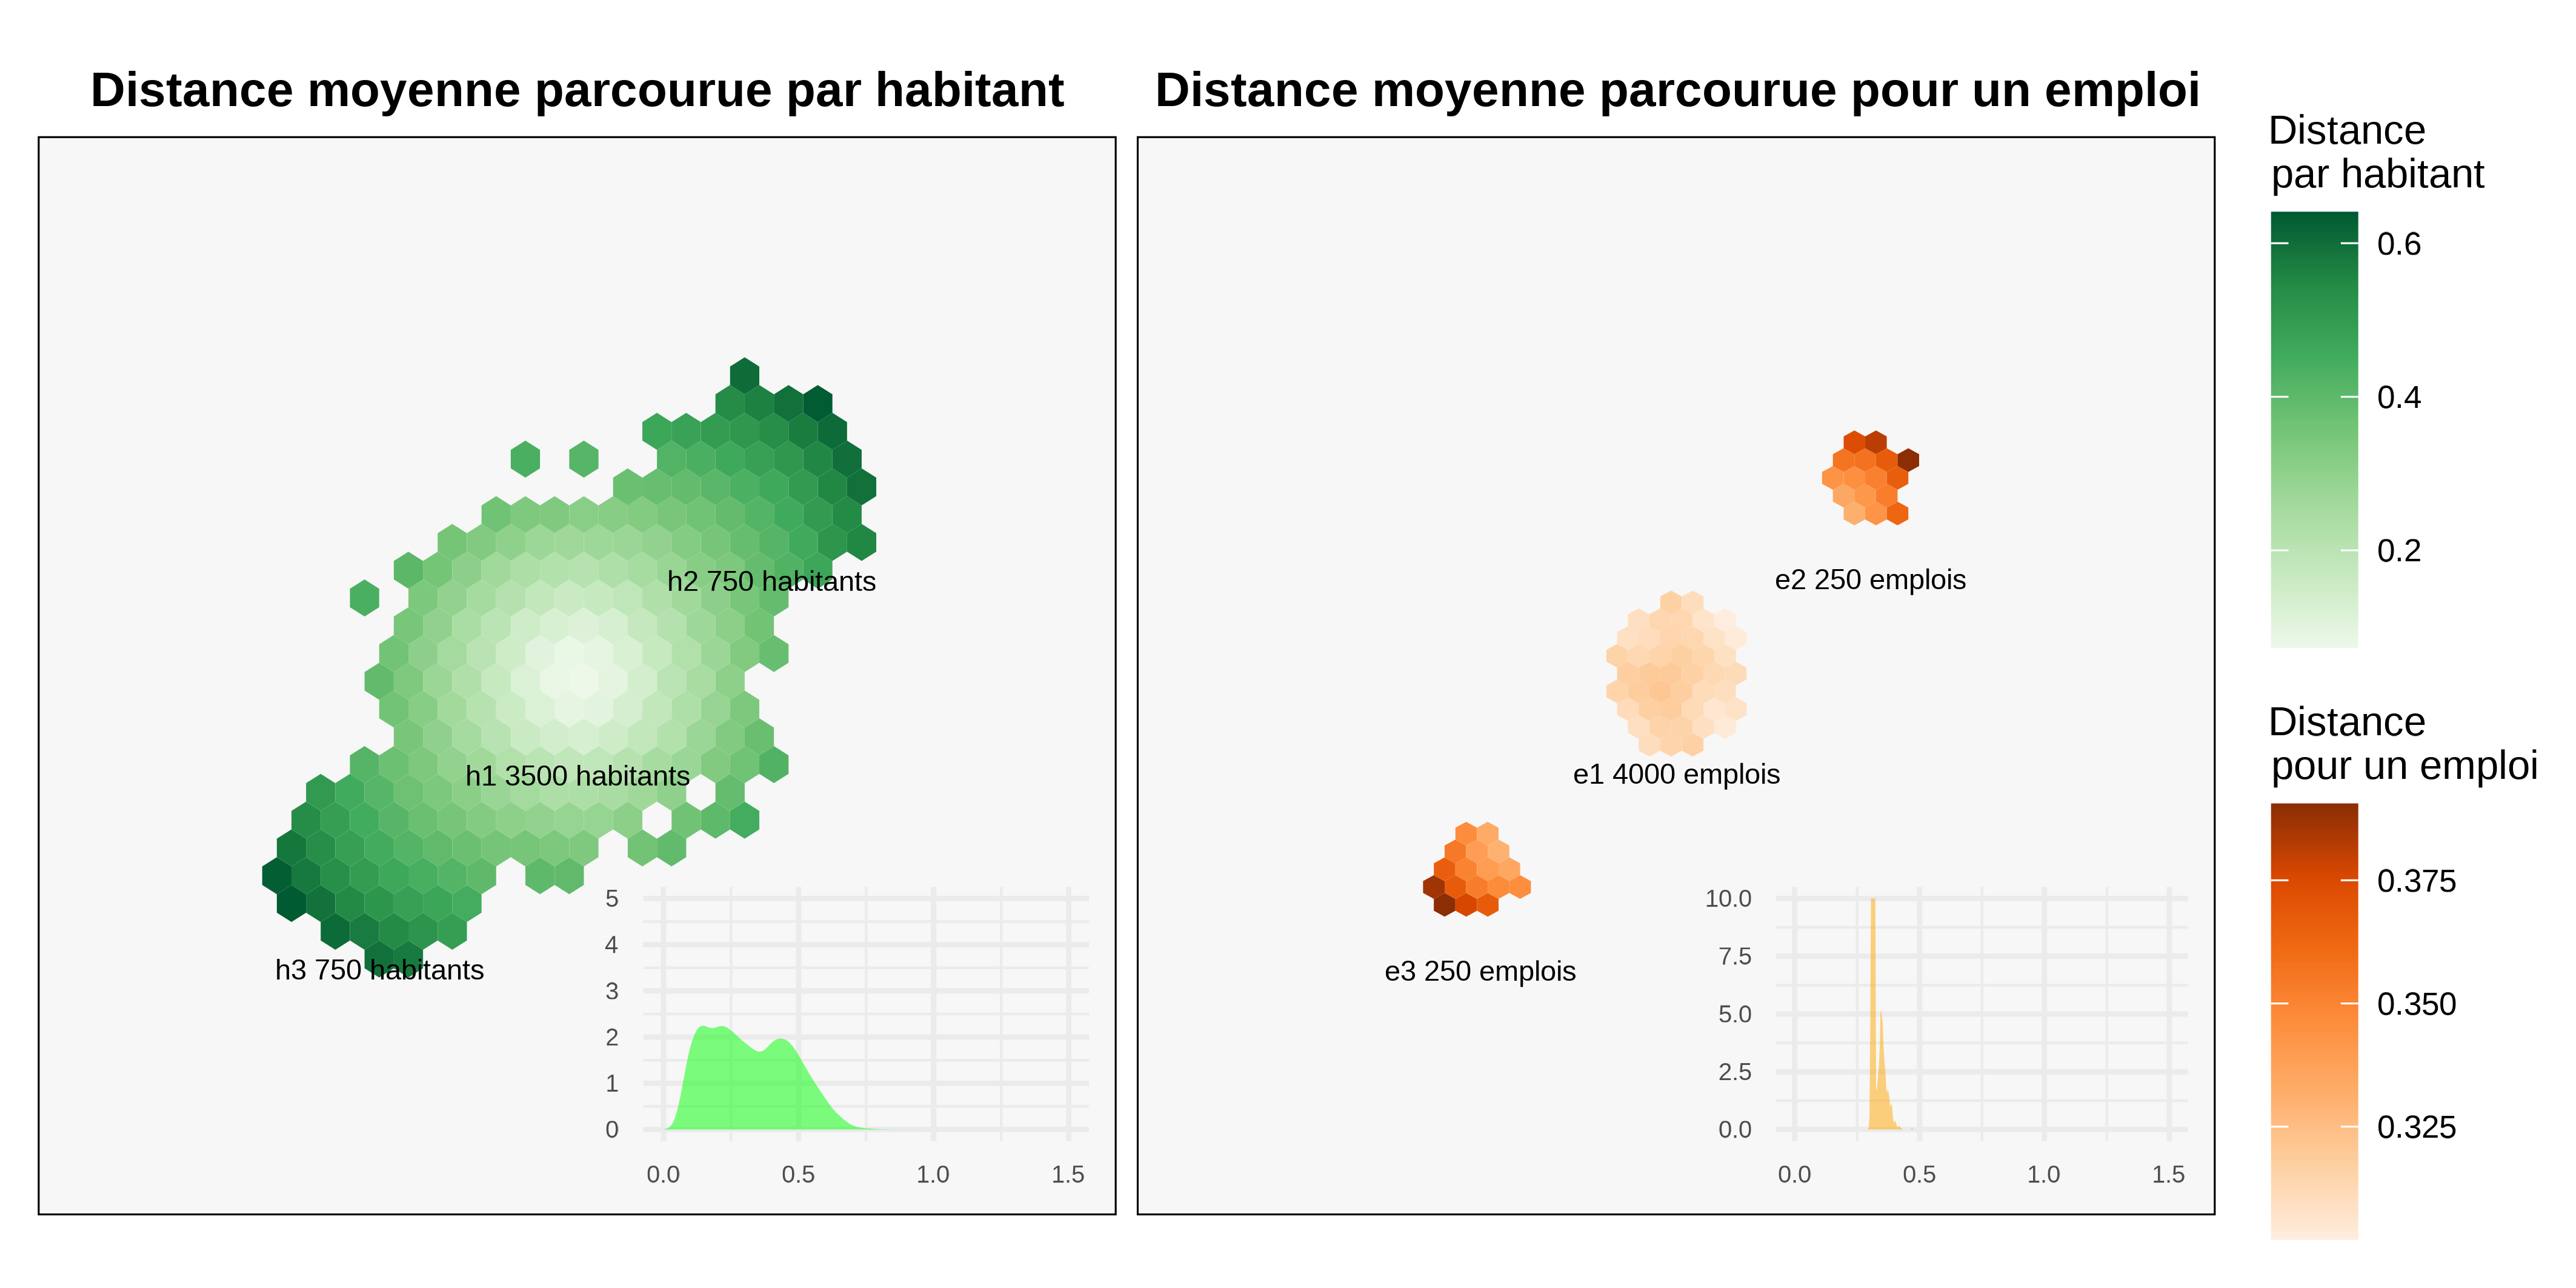
\includegraphics[width=1\textwidth,height=\textheight]{output/gdistances.png}

}

\caption[Distances moyenne par habitant et pour un
emploi]{\label{fig-distances}On représente sur le panneau de
\textbf{gauche} les distances moyennes parcourues par les habitants d'un
héxagone. La vignette présente la densité des trajets en fonction de la
distance(vert). Sur le panneau de \textbf{droite} on représente les
distances moyennes pour atteindre chaque emploi, ainsi que la densité de
ces trajets par distance dans la vignette (orange)}

\end{figure}

Cette première représentation graphique permet de se représenter le
fonctionnement du modèle MEAPS. On peut générer une distribution de
trajets (dans les vignettes de la figure~\ref{fig-distances}). Comme la
majorité des emplois se trouvent dans le pôle central, les distances
moyennes pour les habitants y sont plus faibles que dans les autres
pôles. Le modèle génère un peu de variance à l'intérieur de chaque pôle.
On retrouve l'idée que les hexagones d'habitations les plus excentrées
génèrent des distances plus importantes. La distribution des distances
moyennes pour atteindre un emploi est plus resserrée que celle des
distances parcourues en moyenne par habitant. Les moyennes de ces deux
distributions sont égales (par construction).

On peut construire une table des flux entre chaque pôles
(tableau~\ref{tbl-fluxpoles}). Le premier élément est de noter que les
contraintes aux marges sont parfaitement respectées, ce qui est le
principe de construction de MEAPS, les approximations faites dans
l'algorithme de résolution restant ici inférieures à \(10^{-5}\) au
moins. Par ailleurs, la table de flux confirme le diagnostic précédent.
La plupart des habitants de h1 (95\%) se rendent dans g1 (le même pôle
donc). Ce taux d'``auto-emploi'' est de 10\% à 20\% pour les deux autres
pôles. Cela tient au déséquilibre de localisation des emplois et est une
propriété souhaitée du modèle. Cela explique en partie la distribution
des distances pour les habitants et également le concept réciproque
(distances moyenne vers un hexagone d'emplois).

\hypertarget{tbl-fluxpoles}{}
\begin{longtable}{lrrrr}
\caption{\label{tbl-fluxpoles}flux entre pôles }\tabularnewline

\toprule
 & e1 & e2 & e3 & total \\ 
\midrule
h1 & 2 992 & 81 & 77 & 3 150 \\ 
h2 & 506 & 135 & 34 & 675 \\ 
h3 & 502 & 34 & 140 & 675 \\ 
total & 4 000 & 250 & 250 & 4 500 \\ 
\bottomrule
\end{longtable}

Pour apprécier le comportement du modèle on peut procéder à une
expérience de pensée dans laquelle on éloigne le pôle 3 des deux autres
pôles (la distance entre 1 et 3 passe de 0.7 à 1.2 dans cette
expérience). Le tableau~\ref{tbl-fluxpoles2} est obtenu en re-simulant
le modèle sur la nouvelle géographie. Le résultat est très proche du
modèle précédent. Les flux entre le pôle 1 et 3 sont marginalement
modifiés (de 2 ou 3) alors que ceux entre h1 et e2 ou e3 le sont un peu
plus, traduisant des changements de rangs possibles pour les habitants
de h1 entre e2 ou e3 (qui est plus loin). Ce résultat est conforme à
l'intuition et également une propriété souhaitée du modèle. Les
distributions des distances (sortantes et arrivantes) sont plus
largement modifiées, puisque 3 est plus loin de 1 et 2, comme l'indique
la figure~\ref{fig-distances2}. Les habitants de h1 préfèrent e2 à e3 et
réduisent un peu leur trajets vers e3 mais augmentent leurs distances.
L'accroissement de la saturation sur e2 conduit à des trajets vers e3
(de h1, h2 et h3) qui marque la distribution des distances. la
figure~\ref{fig-denscomp} éclaire ce qui se passe par pôle.

\hypertarget{tbl-fluxpoles2}{}
\begin{longtable}{lrrrr}
\caption{\label{tbl-fluxpoles2}flux entre pôles (pôle 3 plus loin) }\tabularnewline

\toprule
 & e1 & e2 & e3 & total \\ 
\midrule
h1 & 2 992 & 85 & 73 & 3 150 \\ 
h2 & 508 & 133 & 34 & 675 \\ 
h3 & 500 & 33 & 142 & 675 \\ 
total & 4 000 & 250 & 250 & 4 500 \\ 
\bottomrule
\end{longtable}

\begin{figure}[htb]

{\centering 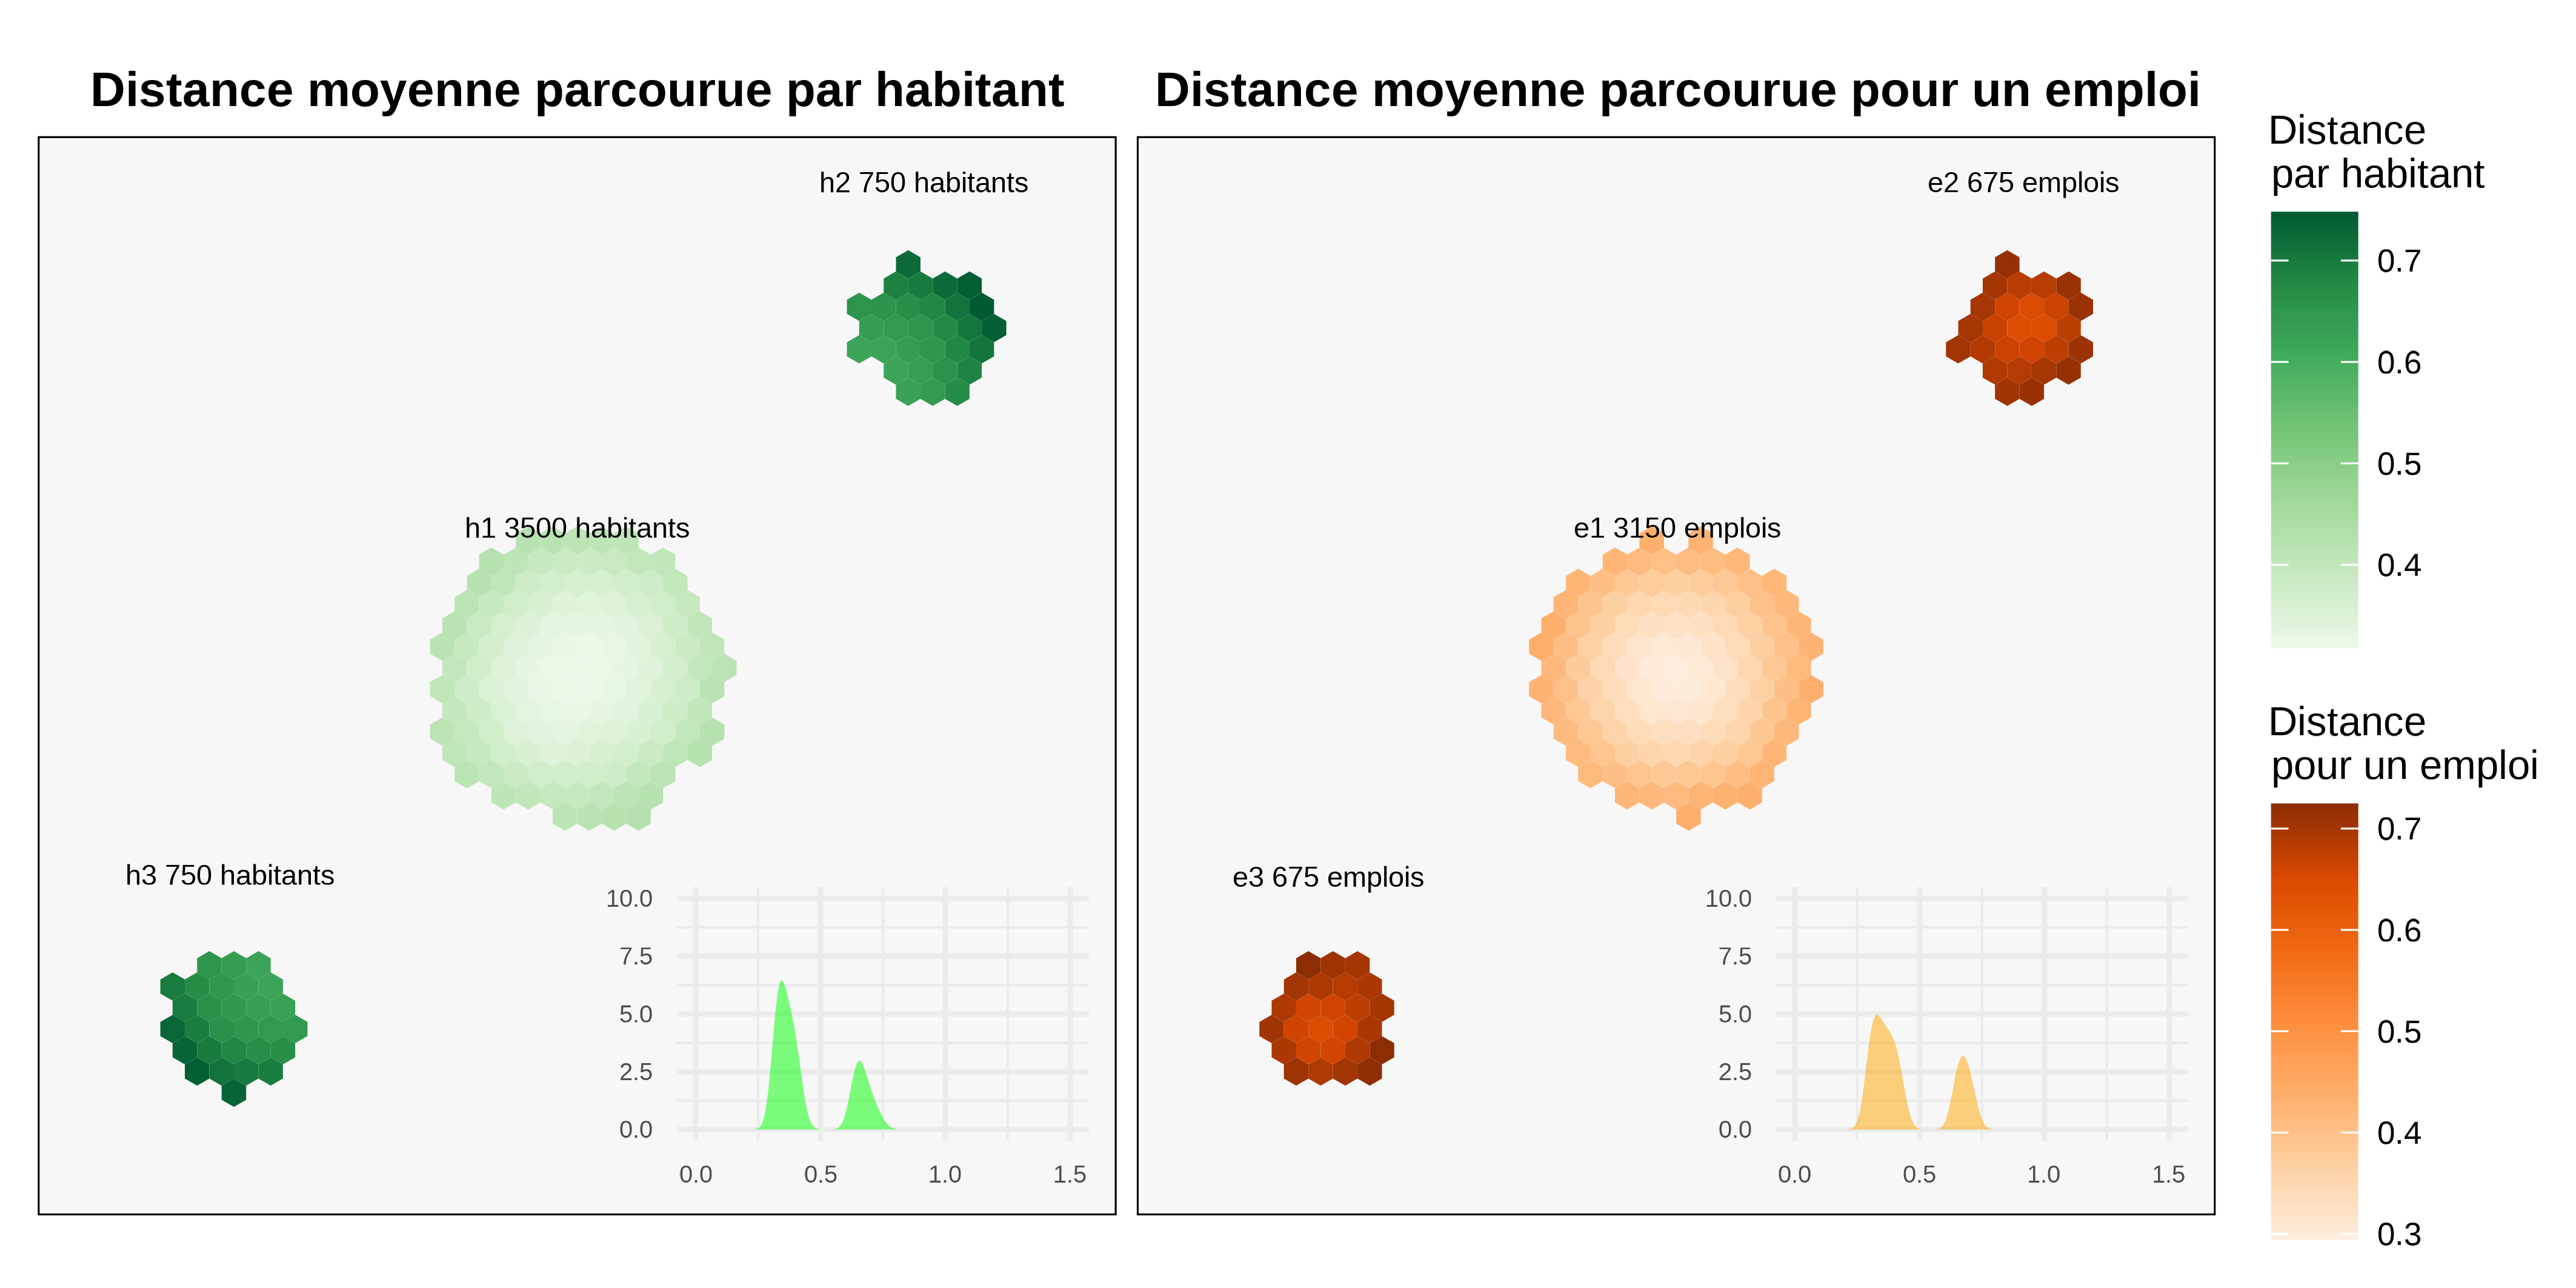
\includegraphics[width=1\textwidth,height=\textheight]{output/gdistances2.png}

}

\caption[Distances moyenne par habitant et pour un emploi (3
éloigné)]{\label{fig-distances2}Le graphique est construit comme le
précédent, le pôle 3 est éloigné de 0.5 (70\% plus loin) par rapport à
1.}

\end{figure}

\begin{figure}[htb]

{\centering 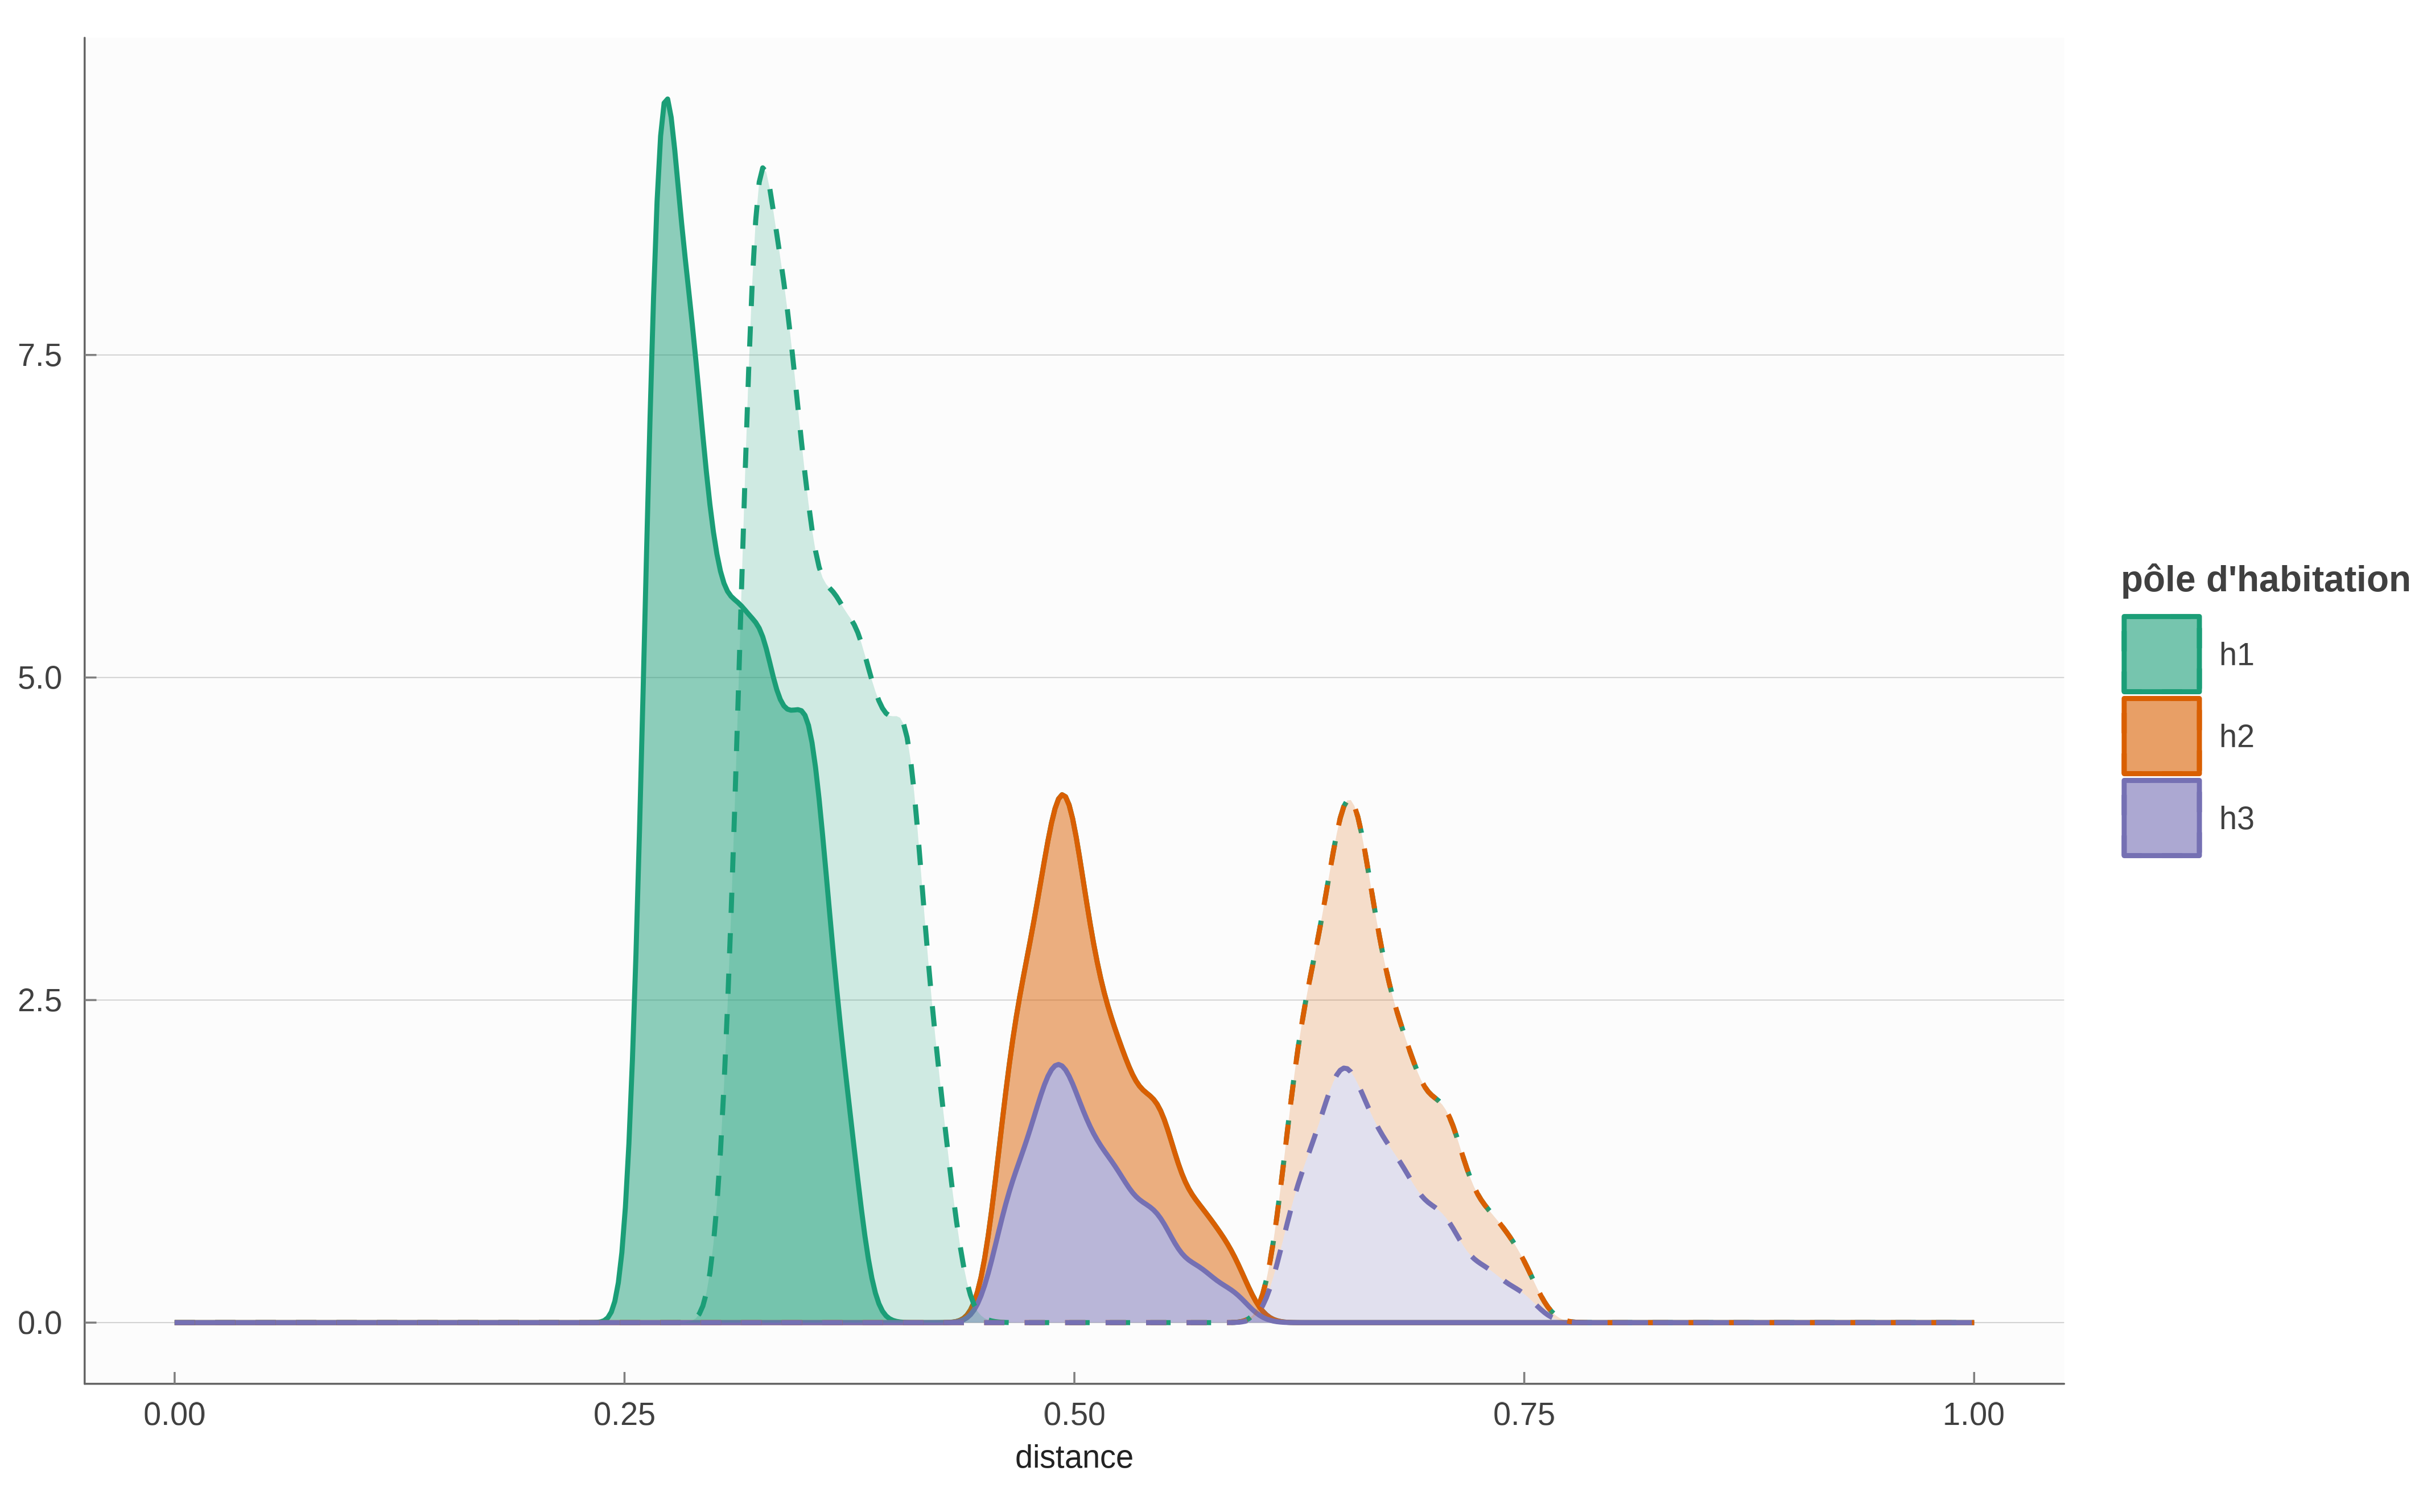
\includegraphics[width=1\textwidth,height=\textheight]{output/gdenshabg.png}

}

\caption[Densités comparées]{\label{fig-denscomp}Densités comparées des
distances parcourues par habitant entre le scénario de référence et le
scénario `pôle 3 plus loin'. Le trait pointillé est utilisé pour le
scénario alternatif.}

\end{figure}

\hypertarget{sec-estimation}{%
\subsection{Procédure d'estimation}\label{sec-estimation}}

Il est possible de modifier les pondérations des probabilités
d'absorption de façon à modifier la table des flux. Ceci est illustré
dans la table suivante où on a doublé pour chaque paire possible de zone
d'habitation et de zone d'emploi la probabilité relative d'absorption.
La configuration géographique est celle de la
figure~\ref{fig-territoire}, avec un centre et deux satellites. Le
centre comporte plus d'emplois que de résidents, ce qui oblige à des
flux entrants dans la zone 1 comme indiqués dans la
tableau~\ref{tbl-fluxpoles}. On parle de doublement relatif de la
probabilité, parce que les contraintes de constance de probabilité de
fuite et de saturation des emplois imposent une réduction des
probabilités d'absorption des autres emplois, ce qui est assuré dans
l'algorithme qui implémente MEAPS.

Le tableau tableau~\ref{tbl-fluxpond} décrit les variations de flux par
rapport à une situation de référence (celle de
tableau~\ref{tbl-fluxpoles}), arrondi à l'entier le plus proche. Il y a
donc \(3 \times 3\) matrices \$3 \textbackslash times 3\$. Chacune des
sous matrice indique les variations de flux pour chaque paire origine
destination et il y a 9 possibilités de doublement de la probabilité
d'absorption qui constitue les lignes et les colonnes de la matrice
englobante. On notera que les sommes des colonnes de chaque sous matrice
sont nulles, ce qui indique le respect des contraintes en ligne et en
colonne.

Conformément à l'intuition et malgré les effets induits par le respect
des contraintes en ligne et en colonne, on observe bien que la paire
zone d'habitation zone d'emploi qui se voit augmentée en probabilité
relative connait des flux supérieurs. Pour compenser ces flux
supérieurs, dans la même colonne, c'est-à-dire pour les flux en
provenance des autres zones d'habitation, on constate systématiquement
une diminution des flux en provenance des autres zones d'habitation.
Symétriquement un accroissement des flux de la zone d'habitation \(i\)
vers la zone d'emploi \(j\) induit toujours une diminution des flux de
\(i\) vers les autres zones d'emploi.

\hypertarget{tbl-fluxpond}{}
\begin{longtable}{l|lrrrrrrrrr}
\caption{\label{tbl-fluxpond}Modification de la probabilité d'absorption par groupe. Le tableau
représente l'écart entre lesd flux obtenus pour une probabilité
d'absorption doublée pour la zone i d'habitation et la zone j d'emploi,
pour chaque paire de zones habitation/emploi. La première matrice en
haut à gauche indique donc que le flux entre la zone 1 d'habitation et
la zone 1 d'emploi est accru de 39 lorsque la probabilité d'absorption
reletive est doublée. Pour compenser ce flux plus important entre 1 et
1, le flux en la zone d'habitation 2 et l'emploi 1 est réduit de 20, ce
qui implique à son tour que ceux entre 2 et 2 et entre 2 et 3
s'accroissent. }\tabularnewline

\toprule
\multicolumn{1}{l}{} &  & \multicolumn{3}{c}{e1} & \multicolumn{3}{c}{e2} & \multicolumn{3}{c}{e3} \\ 
\cmidrule(lr){3-5} \cmidrule(lr){6-8} \cmidrule(lr){9-11}
\multicolumn{1}{l}{} &  & e1 & e2 & e3 & e1 & e2 & e3 & e1 & e2 & e3 \\ 
\midrule
h1 & h1 & 39 & -20 & -19 & -28 & 31 & -2 & -29 & -2 & 31 \\ 
 & h2 & -20 & 16 & 4 & 25 & -26 & 1 & 4 & 1 & -5 \\ 
 & h3 & -19 & 4 & 15 & 3 & -5 & 2 & 25 & 1 & -26 \\ 
\midrule
h2 & h1 & -34 & 29 & 5 & 33 & -33 & -1 & 3 & 5 & -7 \\ 
 & h2 & 41 & -34 & -7 & -37 & 38 & -1 & -8 & -6 & 13 \\ 
 & h3 & -6 & 5 & 2 & 4 & -5 & 1 & 5 & 1 & -6 \\ 
\midrule
h3 & h1 & -35 & 6 & 29 & 2 & -7 & 5 & 34 & -3 & -31 \\ 
 & h2 & -6 & 1 & 5 & 5 & -6 & 1 & 3 & 3 & -6 \\ 
 & h3 & 41 & -7 & -34 & -7 & 13 & -6 & -37 & 0 & 37 \\ 
\bottomrule
\end{longtable}

Une propriété intéressante des matrices de la tableau~\ref{tbl-fluxpond}
est que les 9 matrices \(3 \times 3\) forment un espace vectoriel de
dimension 4\footnote{Les valeurs propres de la matrice \(9 \times 9\)
  constituée des 9 vecteurs colonnes des 9 matrices ``dérivées'' sont
  (133.3, 97.3, -28.6, 22.0, 0, 0, 0, 0, 0). Les 5 valeurs propres
  nulles et les 4 non nulles permettent de conclure que la dimension de
  l'espace vectoriel engendré par les 9 matrices est 4.}. Ceci est
attendu, puisque les contraintes réduisent la dimension de 9
(\(=3\times 3\)) à 4, puisqu'il y a 3 contraintes dans chaque dimension
(lignes et colonnes) et qu'une est redondante (si les somme sur chaque
ligne sont nulles, alors la somme de tous les coefficients est nulle et
donc si les sommes sur deux colonnes sont nulles, la troisième l'est
nécessairement). Cela indique que, au moins localement (au voisinage de
la matrice de flux calculée en tableau~\ref{tbl-fluxpoles}), il est
possible de modifier les probabilités d'absorption pour atteindre
n'importe quelle matrice de flux. A l'approximation linéaire près, il
est donc possible de reproduire n'importe quelle structure de flux
agrégés par un jeu de paramètres saturant exactement la dimension de
cette structure de flux. Cette propriété permet d'envisager différentes
approches d'estimations, suivant les données dont on dispose et du
nombre de degrés de liberté que l'on est prêt à consacrer à la
reproduction des données.

Le temps de calcul peut être assez long du fait de la nécessité de
répéter un grand nombre de tirages, mais la section suivante (
Section~\ref{sec-ergemp}) montre que ce nombre peut rester raisonnable.
Une estimation de ce type est mise en oeuvre par une procédure itérative
dans la section Section~\ref{sec-rochelle}, permettant de reproduire à
l'aide de MEAPS les données issues de l'enquête mobilités
professionnelles INSEE (2022a) avec un schéma de calcul qui peut se
mettre facilement en œuvre.

\hypertarget{sec-ergemp}{%
\subsection{Ergodicité en pratique}\label{sec-ergemp}}

L'utilisation de données synthétiques permet de tester simplement
l'hypothèse d'ergodicité. On a conjecturé que les différentes grandeurs
moyennes sur les permutations \(u\) étaient assimilables à des
observations, éventuellement répétées. A ce stade de simulations
synthétiques nous ne confrontons pas le modèle à des observations (voir
Section~\ref{sec-rochelle}), mais nous allons montrer que l'estimation
des valeurs moyennes ne demande pas l'examen des \(I!\) permutations
possibles\footnote{Par la formule de Stirling
  \(log_{10}(I!) \approx (n +1/2)log_{10} n +log_{10}\sqrt{2} - n log_{10}e \approx 5\times10^5\)
  pour \(I=10^5\), ce qui fait un nombre de grande taille.} et peut se
contenter d'une agrégation spatiale et de quelques tirages de
permutations.

Pour illustrer cette propriété, nous répétons les simulations du modèle
pour plusieurs tirages de priorités (notés \(u\) dans la section
Section~\ref{sec-erg}). En prenant la moyenne sur un échantillon de
\(u\), on peut construire un estimateur des grandeurs moyennes et
montrer qu'avec un échantillon petit par rapport à \(I!\), on peut les
estimer avec fiabilité et dans un temps raisonnable. Cette propriété
sera montrée sur la structure géographique particulière que nous avons
synthétisée, sans que cela permette de le généraliser avec certitude. Il
existe sans doute des configurations spatiales pathologiques qui
contredisent cette conjecture.

La figure~\ref{fig-emperg} illustre les processus stochastiques à
l'œuvre dans le modèle et leur résolution par la moyennisation sur les
tirages possibles. On applique le modèle en tirant aléatoirement des
permutations de priorité de choix. On représente alors pour quelques
hexagones d'habitation (tirés au sort) l'ensemble des choix de
destination (carroyés dans les hexagones). Le carroyage opère déjà une
moyennisation puisque chacun des individus de chaque hexagone a un ordre
de priorité différent. On représente alors les quantités d'emplois (la
probabilité de choisir comme emploi un emploi qui se trouve dans
l'hexagone d'arrivée). Les lignes blanches illustrent la dépendance au
tirage de priorité. Mais au bout de quelques tirages, ces probabilités
convergent en moyenne. Pour simuler le modèle, il n'est pas nécessaire
(en toute vraisemblance) de parcourir l'univers entier des permutations.

\begin{figure}[htb]

{\centering 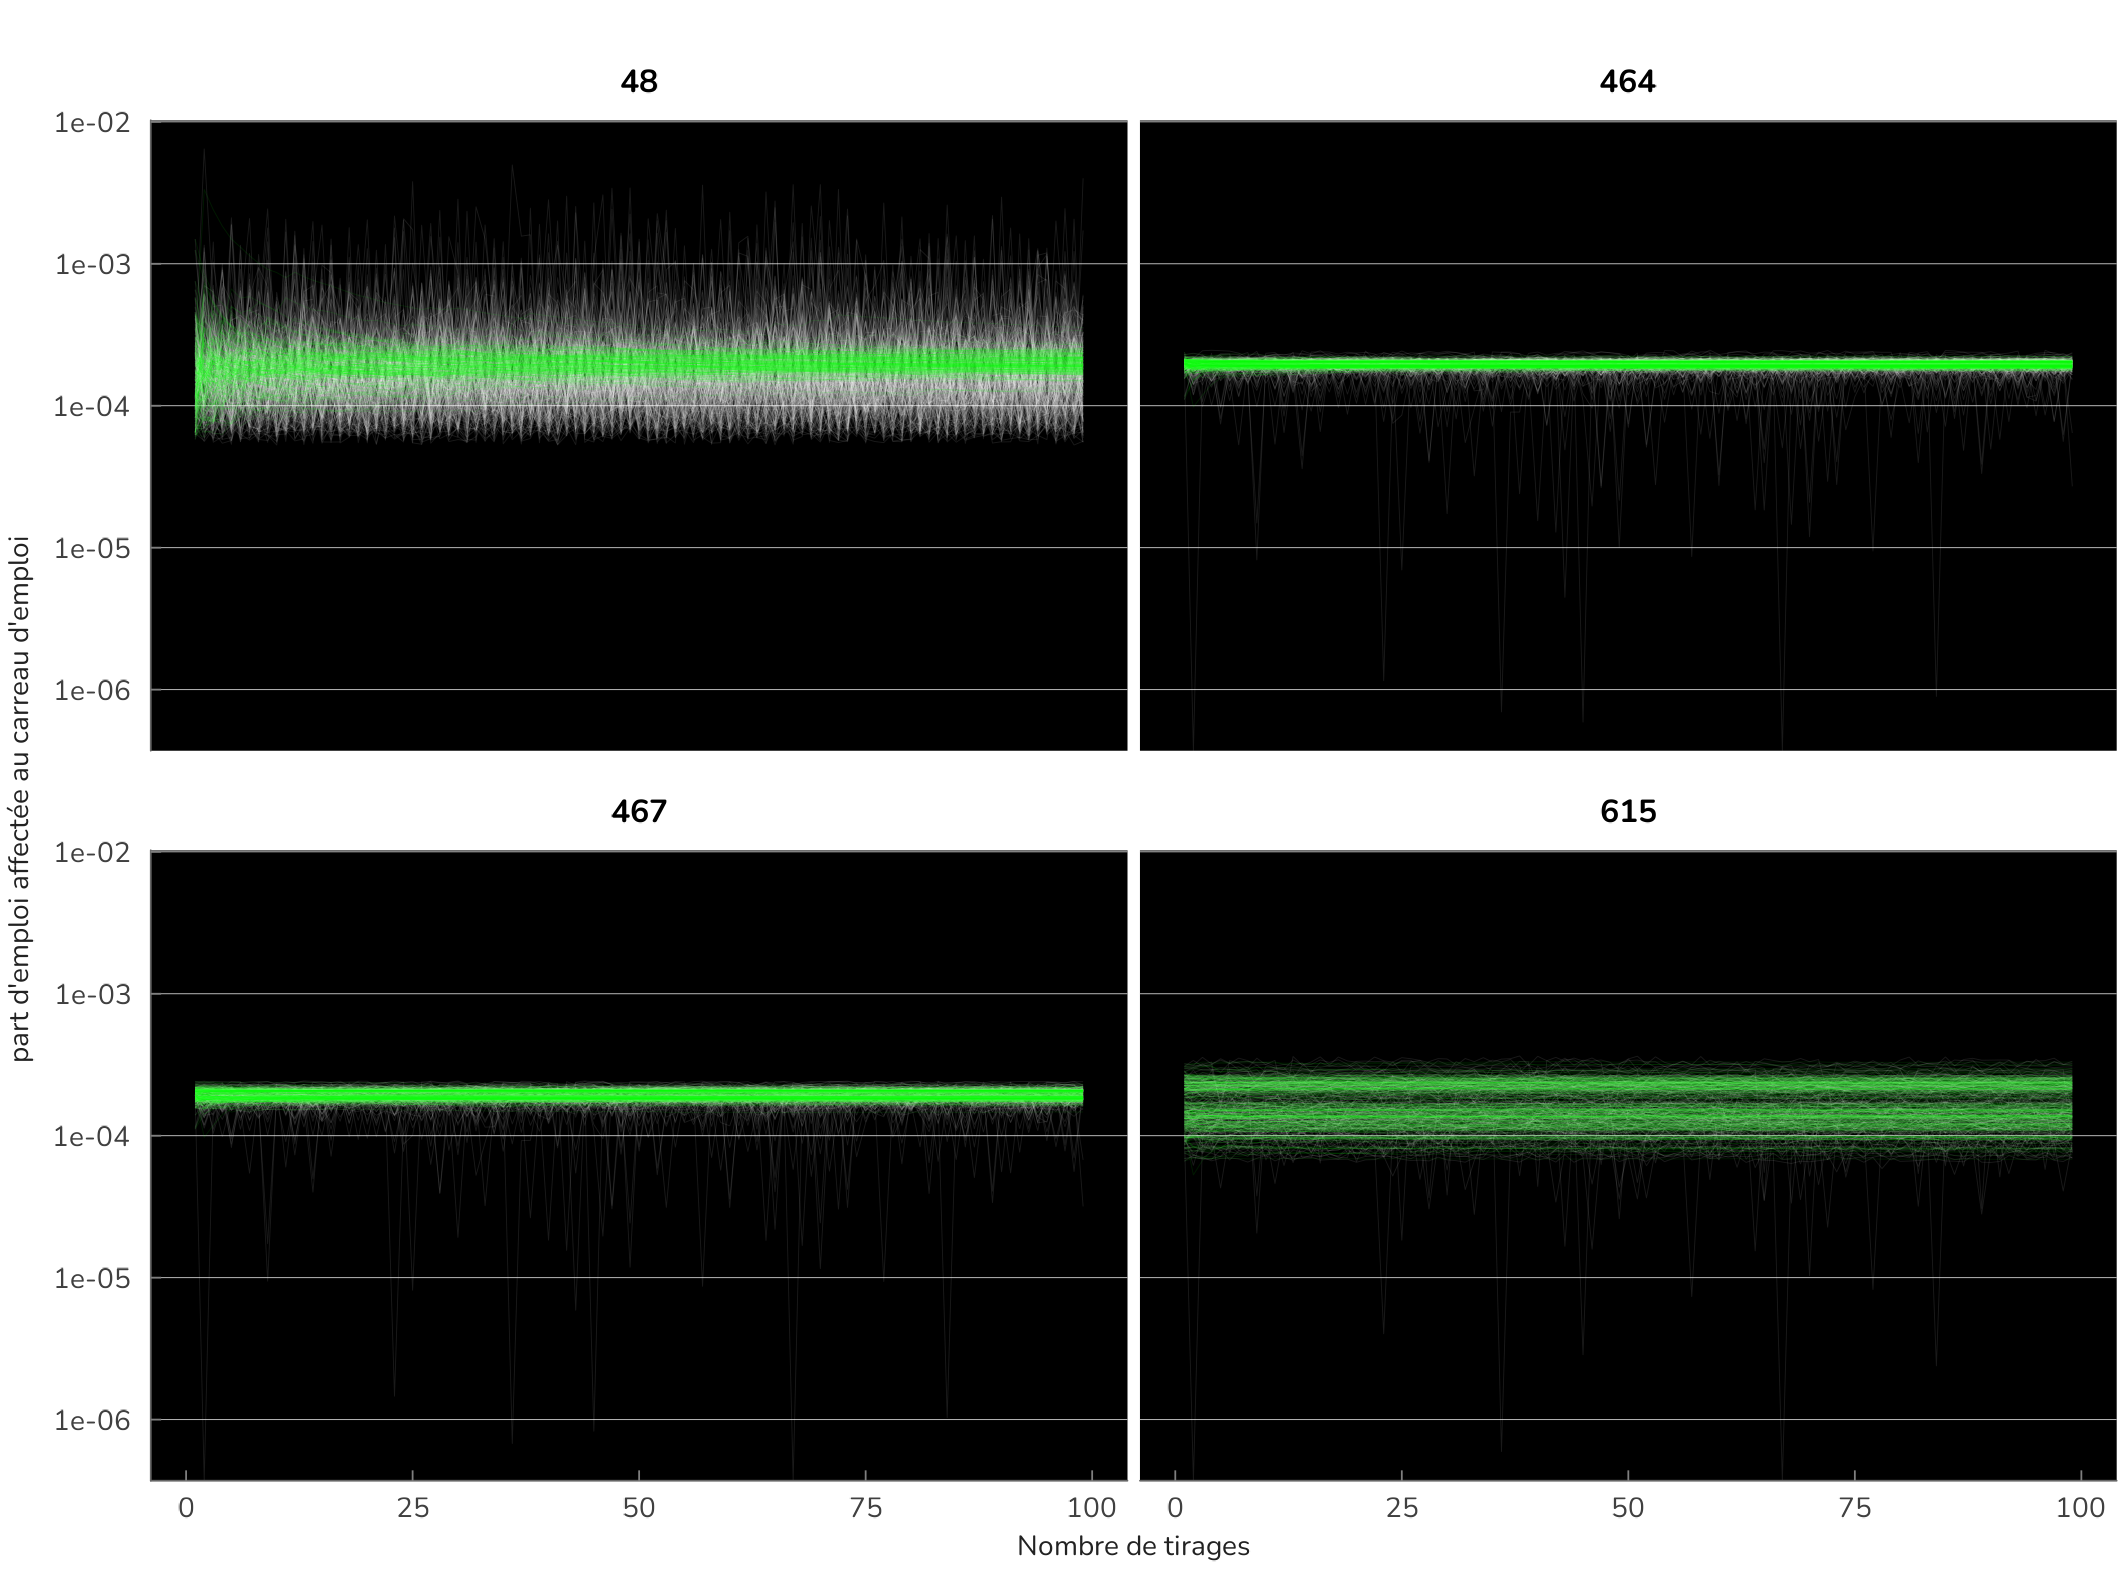
\includegraphics[width=1\textwidth,height=\textheight]{output/gemploi_erg.png}

}

\caption[Affectation de l'emploi pour des carreaux de
départ]{\label{fig-emperg}Chaque ligne blanche représente pour un
carreau de départ et d'arrivée (tous les carreaux d'arrivée sont
représenté par une ligne, pour une sélection aléatoire de 4 carreaux de
départ) la probabilité de prendre l'emploi dans le carreau d'arrivée en
fonction du tirage aléatoire. Les lignes vertes représentent cette même
probabibilité prise en moyenne sur les tirages cumulés. L'échelle de
l'axe des y est logarithmique.}

\end{figure}

Le schéma de saturation et de priorité est illustré par la
figure~\ref{fig-rangerg} ci-dessous. Pour chaque carreau d'arrivée (un
emploi), on représente le rang moyen (gauche) et son écart type (droite)
au moment de la saturation. La caractère stochastique découle du tirage
aléatoire de l'ordre de chaque individu (les carreaux de départ). Pour
la plupart des emplois, le rang moyen de saturation ergodique est
atteint très rapidement. Trois bandes blanches apparaissent sur le
graphique. Pour beaucoup d'emplois le rang moyene est le même et
relativement élevé. Pour quelques emplois le temps de convergence vers
un état indépendant des tirages est plus long. Pour un grand nombre de
destinations, l'écart type est faible. Ces graphiques confirment qu'à
quelques exceptions, l'état du système est stable après quelques tirages
et le calcul de la moyenne.

\begin{figure}[htb]

{\centering 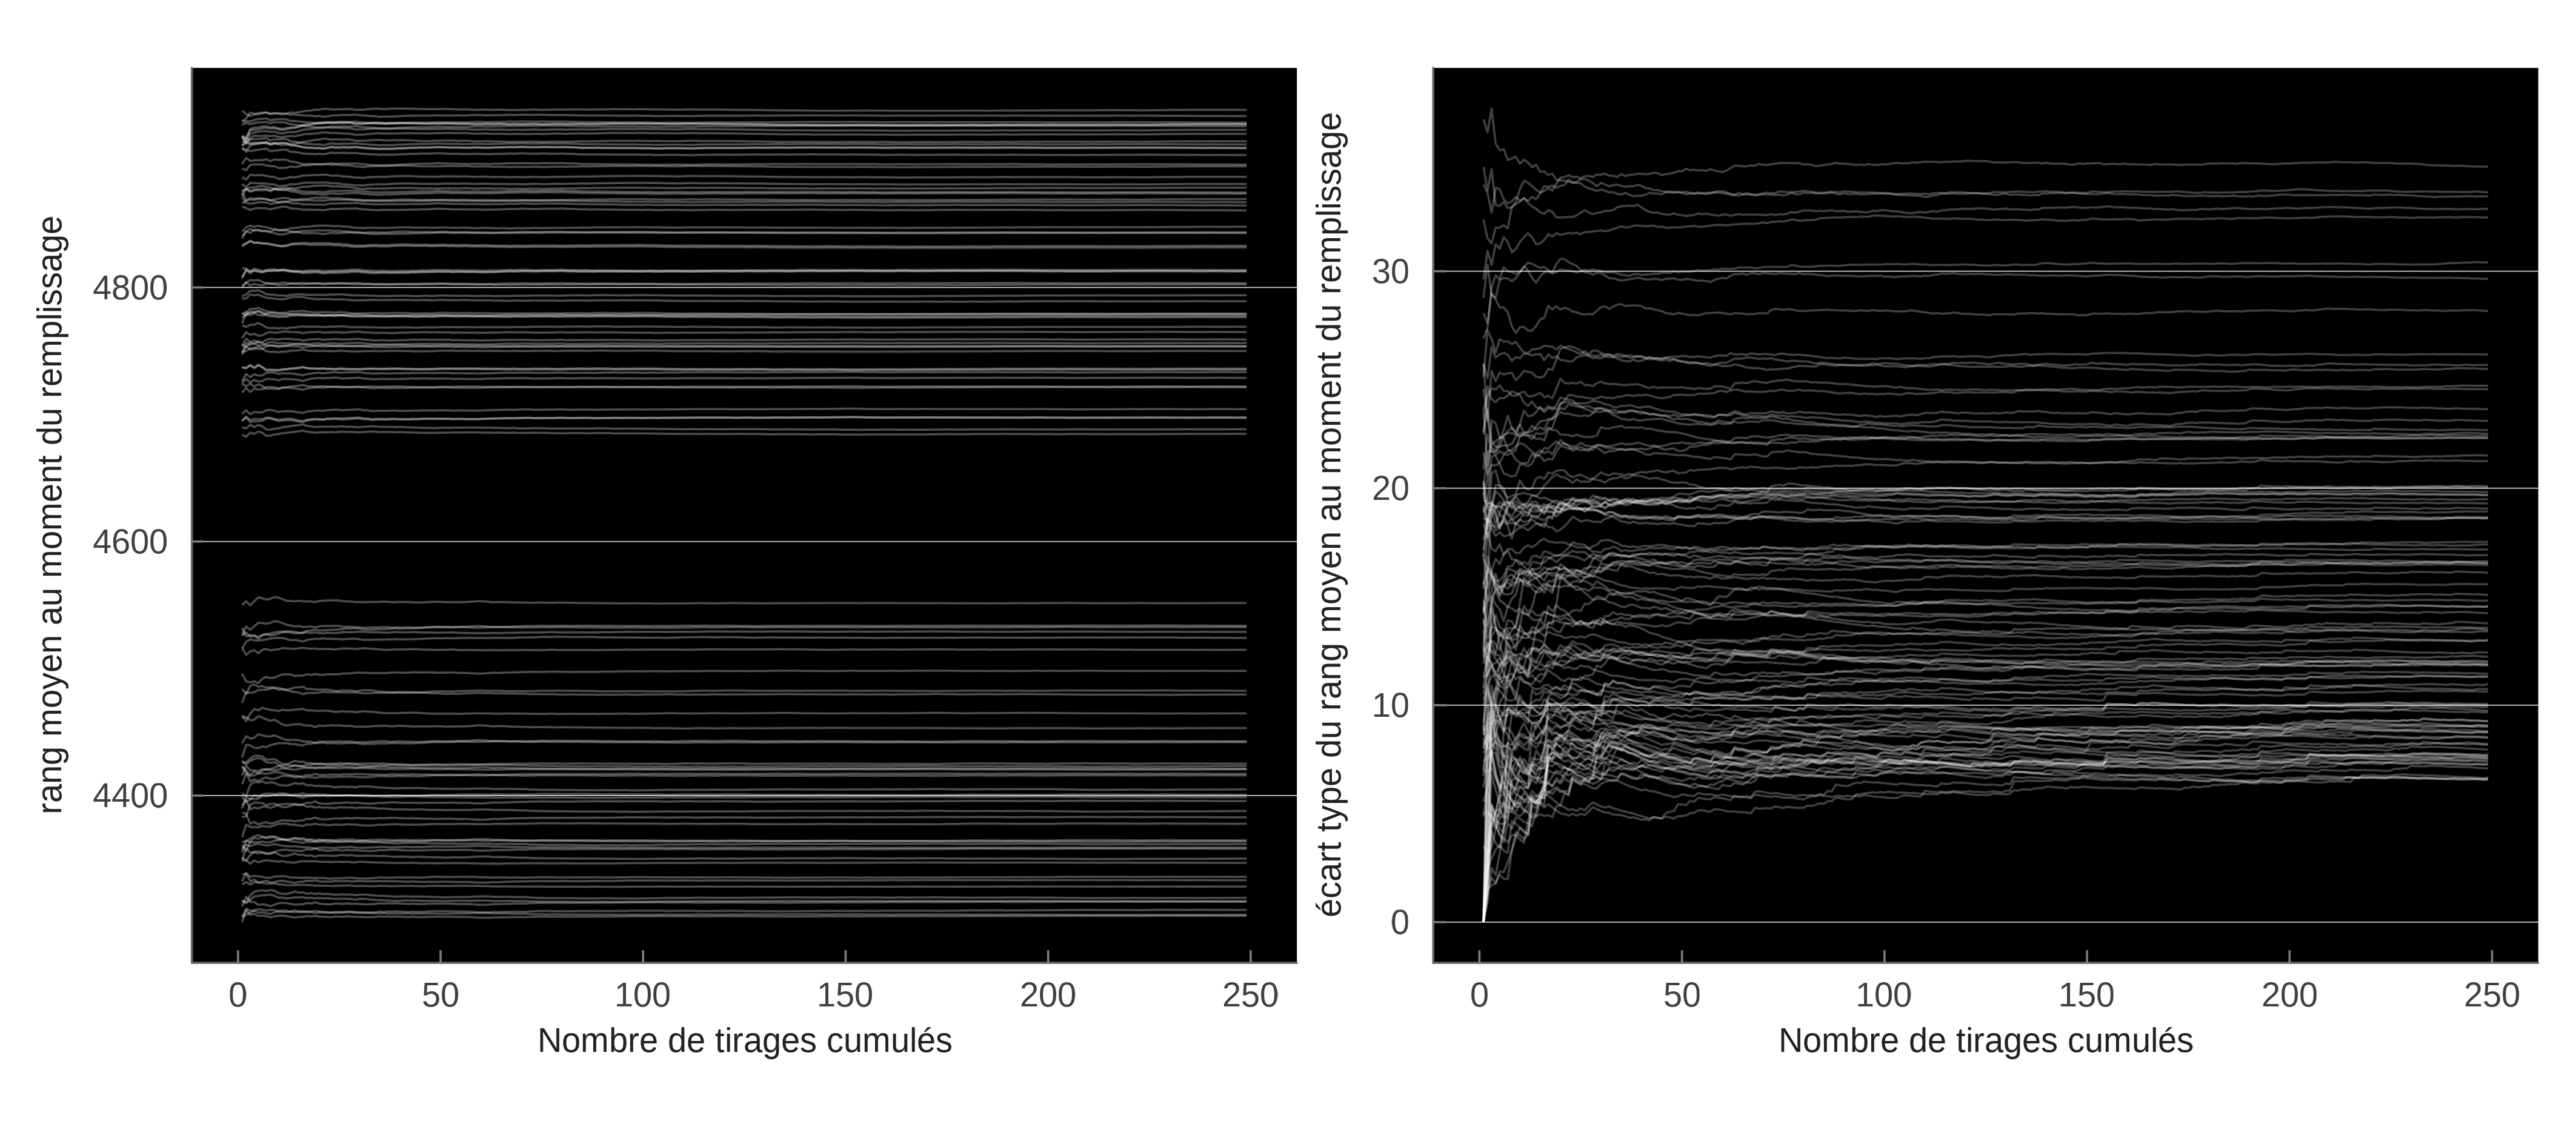
\includegraphics[width=1\textwidth,height=\textheight]{output/g_rangns.png}

}

\caption[Rang au moment de la saturation]{\label{fig-rangerg}Chaque
ligne blanche représente pour un carreau d'arrivée (tous les carreaux
d'arrivée sont représenté par une ligne) le rang moyen (panneau gauche)
et l'écart type du rang (panneau de droite).}

\end{figure}

La figure~\ref{fig-fluxerg} est construite en simulant 500 tirages de
priorité et en calculant les flux entre pôles. A ce niveau d'agrégation,
plus aucune variance ne subsiste et un très faible nombre de tirages est
nécessaire pour pouvoir quantifier les flux. On a la une illustration de
la nature ergodique du modèle. L'estimation telle que présentée en
Section~\ref{sec-estimation} peut ainsi fonctionner y compris si on ne
réalise que quelques tirages aléatoires des priorités.

Le rang moyen au moment de la saturation est un objet qui peut être
utilisé pour construire un indicateur localisé de tension.

\begin{figure}[htb]

{\centering 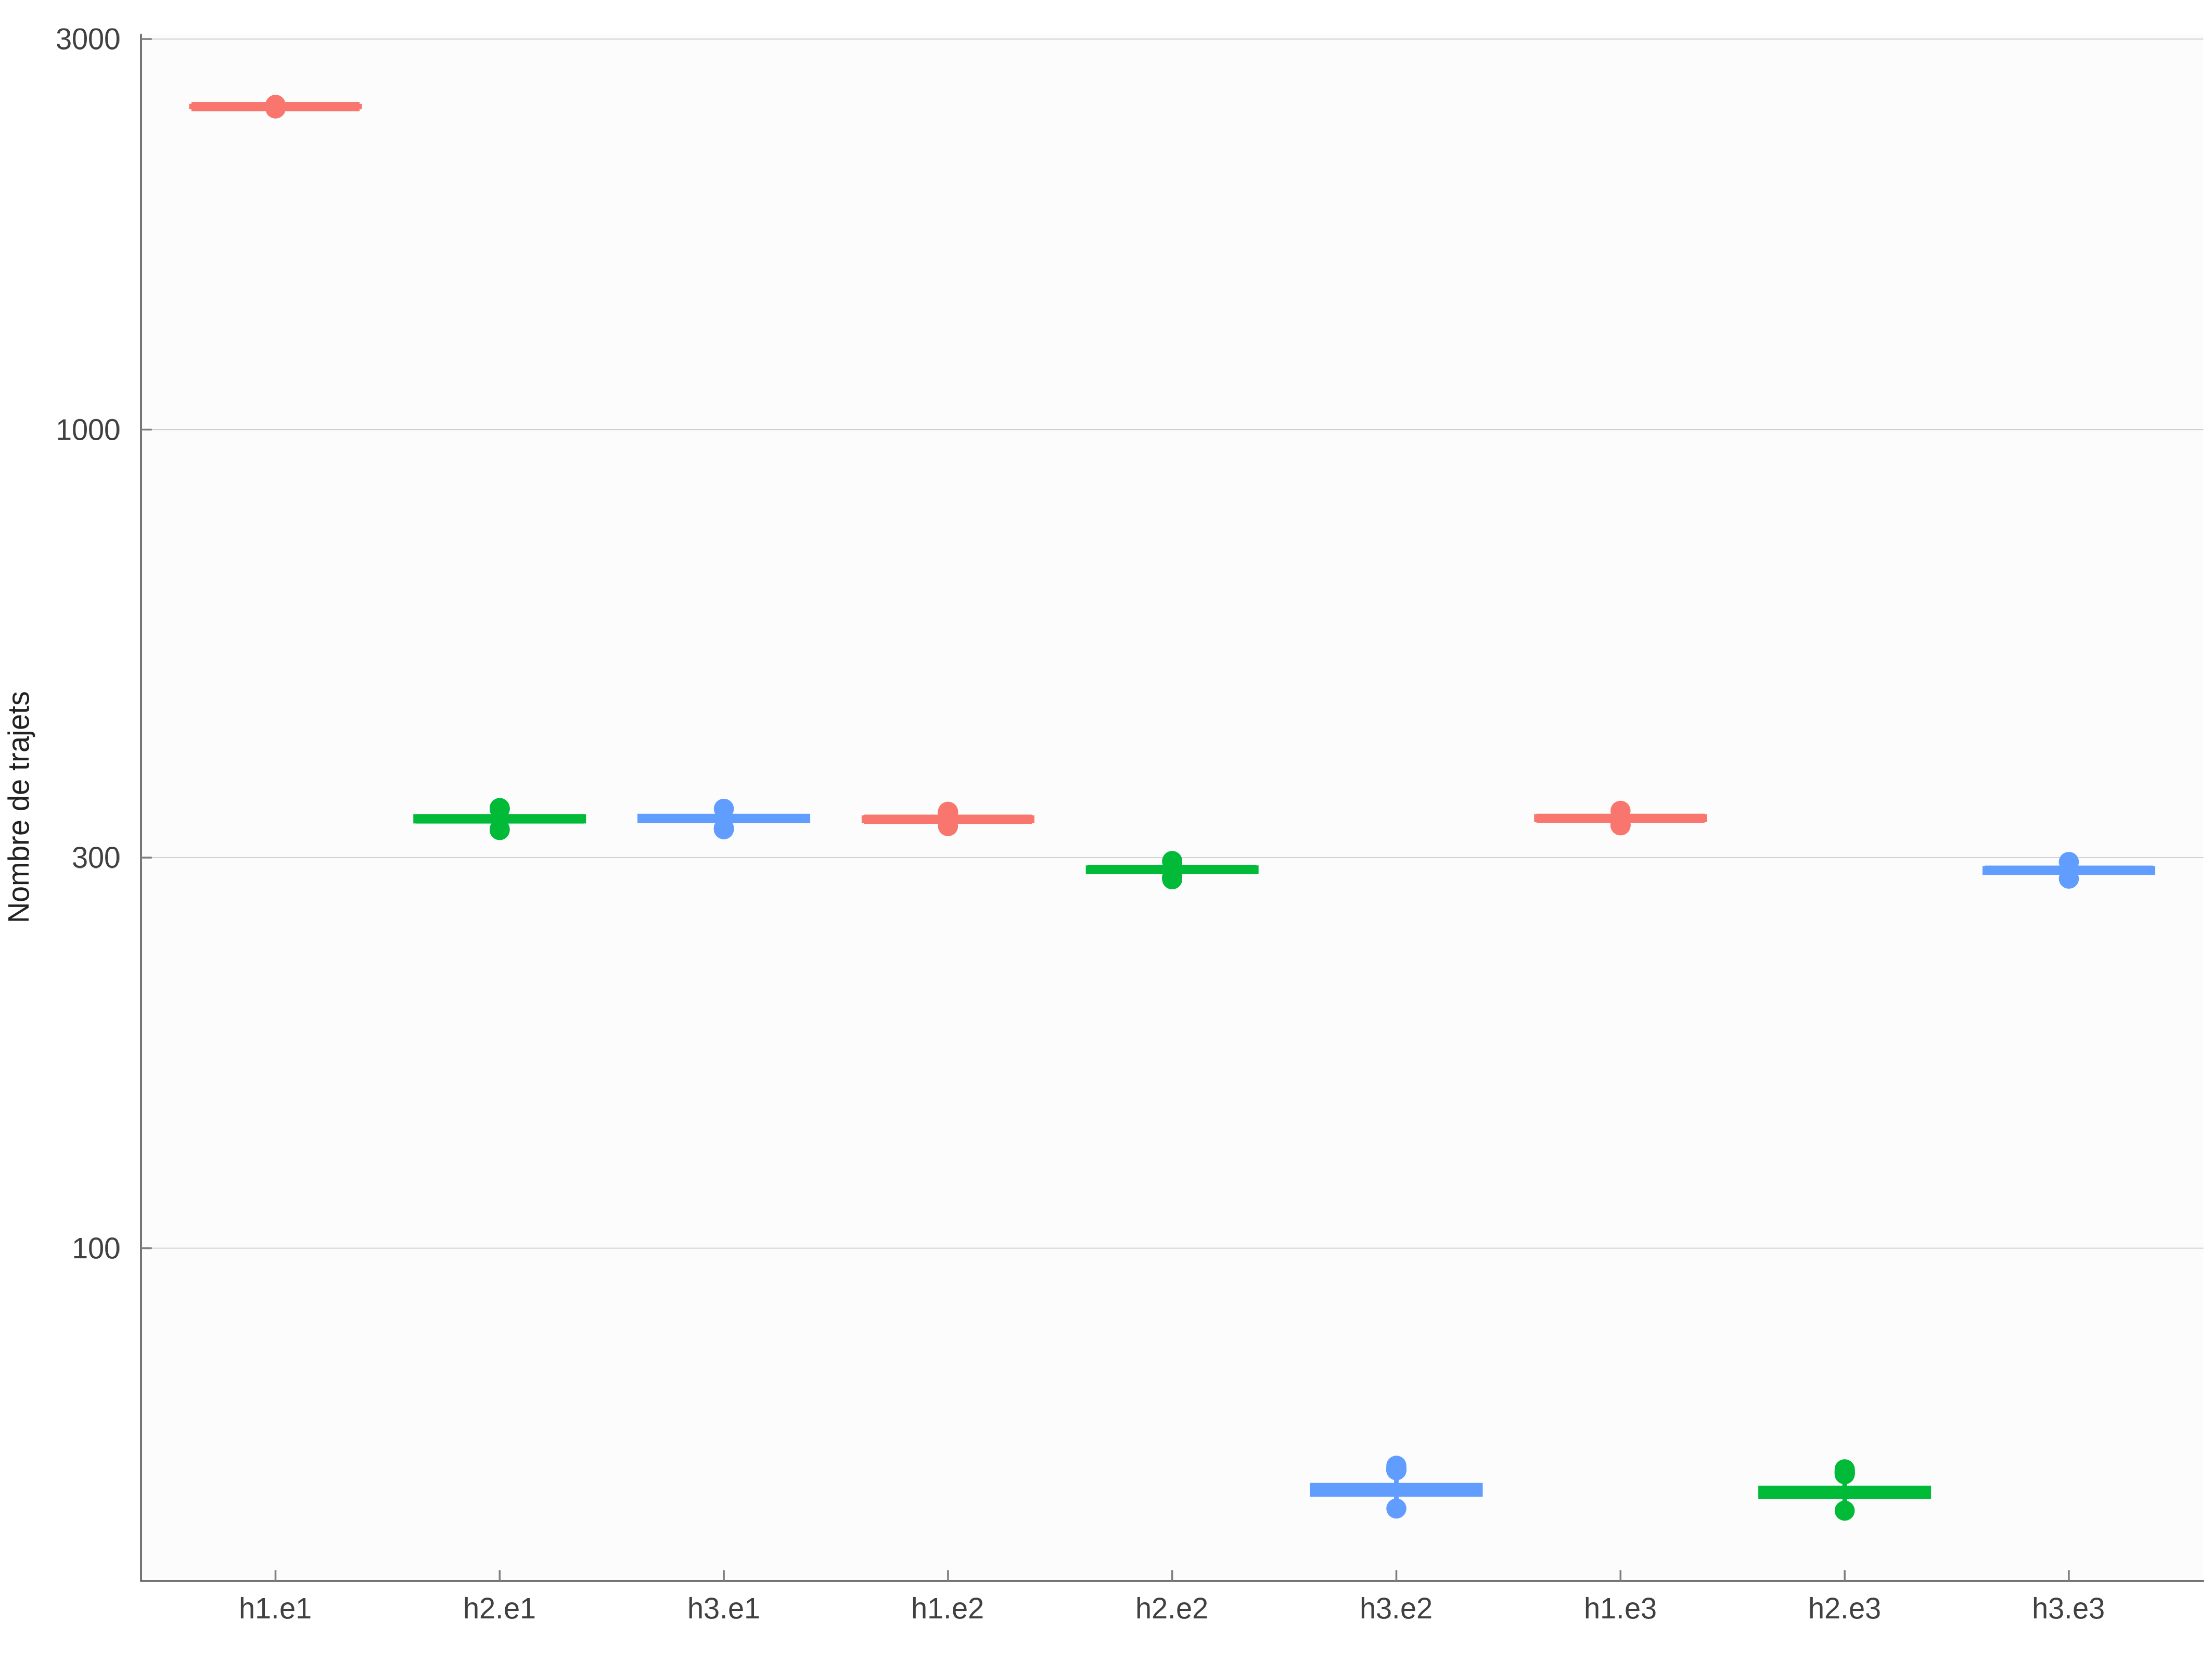
\includegraphics[width=1\textwidth,height=\textheight]{output/gfluxs.png}

}

\caption[Flux entre pôles, distribution]{\label{fig-fluxerg}On simule
500 tirages de priorité tirés au sort et on calcule les flux impliqués
par le modèle entre pôles. A ce niveau d'agrégation, les flux sont
pratiquement invariants d'un tirage à l'autre à l'exception des `petits'
flux. L'échelle de l'axe des y est logarithmique.}

\end{figure}

\hypertarget{sec-rochelle}{%
\section{Une application à l'agglomération de La
Rochelle}\label{sec-rochelle}}

Nous proposons ici une première application de MEAPS à l'agglomération
de la Rochelle. Cette application est issue d'un travail de
quantification de scénarios de politiques publiques visant à réduire
l'empreinte carbone associée aux mobilités quotidiennes et au secteur
résidentiel. La quantification demande à la fois de produire une
cartographie très fine des émissions, en procédant par interpolation à
partir de données plus macroscopiques mesurées par ailleurs et d'être en
mesure de produire des évaluations des différences d'émissions
localement et à l'échelle du territoire selon les différents scénarios.
Nous présentons ici deux familles de scénarios pour lesquelles MEAPS a
été mobilisé :

\begin{itemize}
\item
  Des scénarios de localisation de l'emploi : nous projetons la
  distribution des trajets en utilisant MEAPS sur deux structures
  spatiales de l'emploi différentes, tout en conservant la même quantité
  d'emploi globale. La différence entre les kilomètres parcourus suivant
  les différents modes dans les deux scénarios permet d'évaluer l'impact
  de la localisation, en distinguant la contribution du changement
  modal, la contribution des changements de distance pure (à mode et
  flux carreaux à carreaux inchangés) et la contribution des changements
  de flux.
\item
  Des scénarios de modification de la structure du réseau de transport.
  Le principe est identique à celui pour la localisation de l'emploi.
  C'est la matrice des distances et des temps qui est modifiée par une
  modification des infrastructures de transports (par exemple une ligne
  de bus en plus). Cette matrice de distance différente induit des temps
  de trajet plus petits mais uniquement pour le mode transport en
  commun. Elle induit un changement modal (plus de transport en commun,
  moins des autres modes) et enfin conduit à un changement des rangs des
  opportunités et donc une redistribution des flux de carreau à carreau.
\end{itemize}

Dans les deux familles de scénarios, les simulations par MEAPS
permettent de construire un contrefactuel et des alternatives à un
niveau fin, croisant la localisation au carreau 200m pour les résidences
(5 456 carreaux pour la Rochelle et le périmètre du SCOT) et les
opportunités (6 326 carreaux dans le périmètre de 33km autour de
l'agglomération de la Rochelle), soit 34,5 millions de flux et de modes.
L'agrégation de ces informations est alors possible à des niveaux plus
généraux pour analyser les impacts. La conversion des kilomètres ou des
minutes en émissions de CO\textsubscript{2} pour la voiture est faite en
appliquant des coefficients de conversion conventionnels, ce qui permet
d'étendre les indicateurs au champ des émissions de gaz à effet de
serre.

\hypertarget{emplois-ruxe9sidents-au-carreau-inspire-200m}{%
\subsection{Emplois, résidents au carreau Inspire
200m}\label{emplois-ruxe9sidents-au-carreau-inspire-200m}}

La carte de la zone considéré est représentée sur la
figure~\ref{fig-zoneslr}. L'analyse est limitée aux résidents du
périmètre du Schéma de COhérence Territoriale (SCOT) et considère les
emplois dans un rayon 33 kilomètres autour de lieux de résidence. Cette
carte est construite à partir des données carroyées de l'INSEE INSEE
(2022b) à la résolution du carreau 200m Inspire\footnote{INfrastructure
  for SPatial InfoRmation in Europe est depuis 2007 une directive pour
  la production de données spatialisées. Inspire définit une grille de
  carroyage et son système de projection harmonisée. C'est ce qui suit
  l'INSEE dans la diffusion des données carroyées. Voir
  https://inspire-geoportal.ec.europa.eu pour la définition de la grille
  et des jeux de données.}. Nous ajoutons à ces données la localisation
de l'emploi sur la même grille en utilisant les fichiers fonciers et les
données d'emplois localisés de INSEE (2022a)\footnote{Une alternative
  est d'utiliser FLORES qui propose une localisation de l'emploi à la
  commune sur la base des DADS. FLORES fournit probablement une donnée
  de meilleure qualité, mais comme nous utilisons ensuite les flux entre
  communes de résidence et d'emploi, pour des raisons de cohérence, il
  est plus logique d'utiliser INSEE (2022a).}. La méthode consiste à
imputer par code NAF\footnote{L'utilisation des codes NAF dans les
  fichiers fonciers pose deux problèmes. L'un est la prise en compte des
  bâtiments publics, qui ne sont pas soumis à la taxe foncière et
  l'autre est l'identification du code NAF de l'usage effectif du local
  lorsque le local est loué.} les emplois de chaque commune selon INSEE
(2022a) aux surfaces professionnelles à la parcelle issues des fichiers
foncier s. Cela permet ensuite de localiser au carreau 200m les emploi
s. Cette méthode est assez grossière, puisqu'en particulier la ratio
personne/surface n'est pas constant d'une entreprise à l'autre, mais
elle fournit une bonne première approximation d'autant que
l'extrapolation ne dépasse pas l'échelle de la commun e. Elle est en
tout cas très supérieure à une imputation uniform e.

\begin{figure}[htb]

{\centering 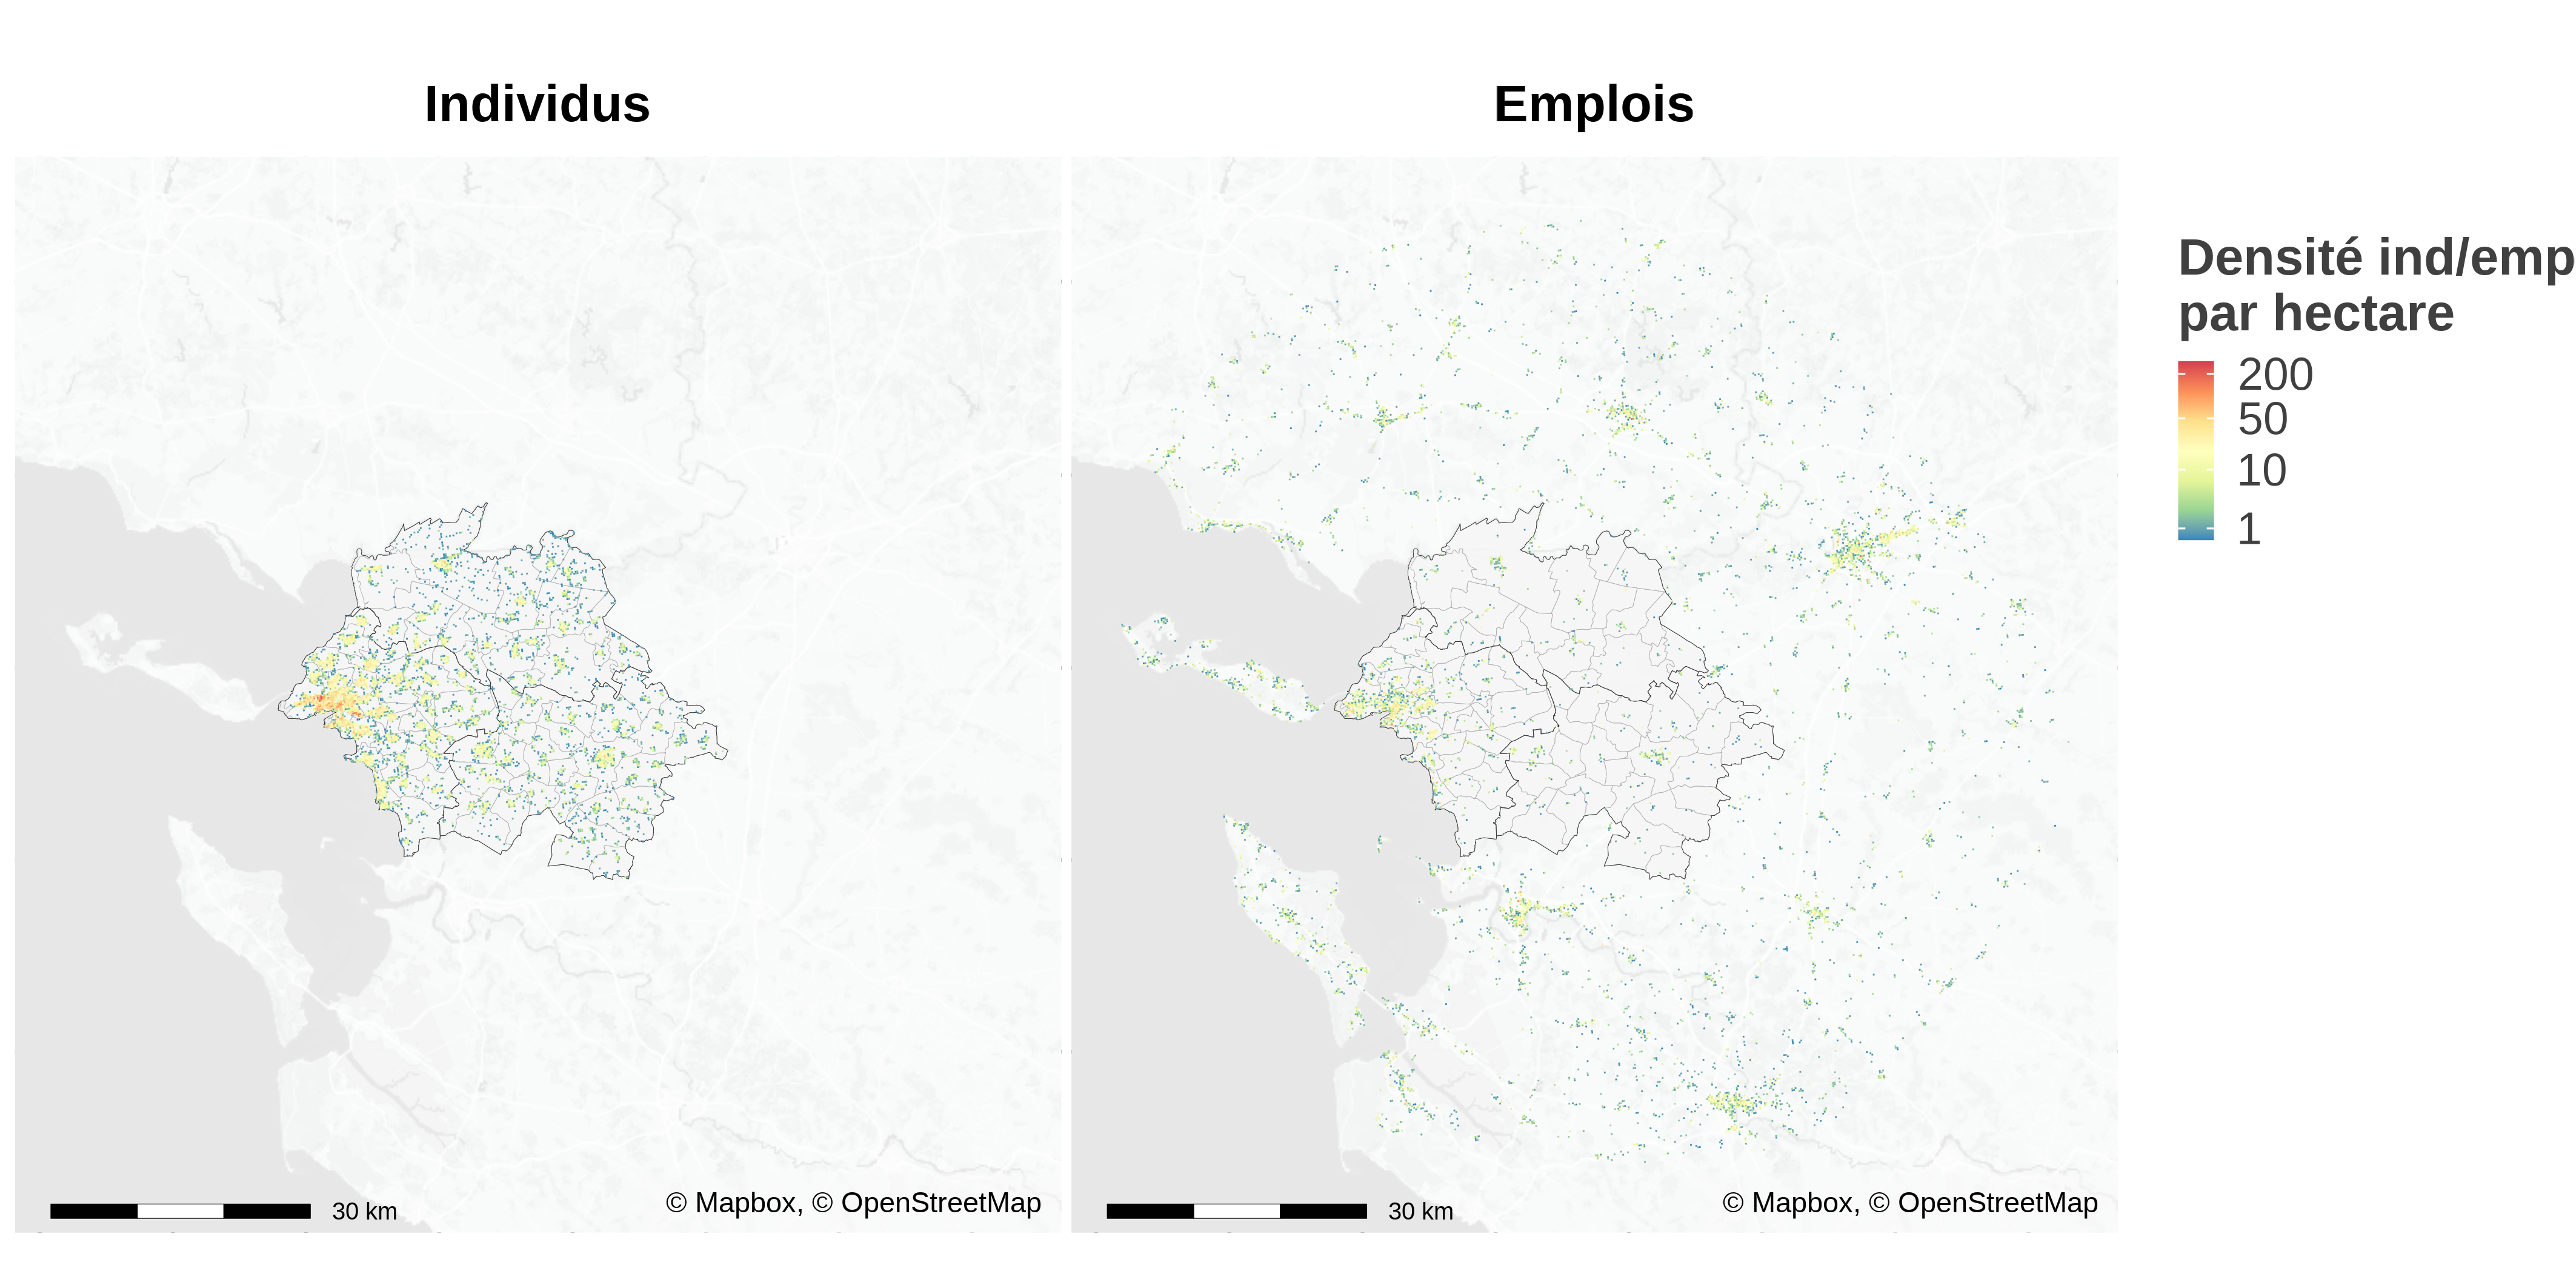
\includegraphics[width=1\textwidth,height=\textheight]{output/popemp.png}

}

\caption[Localisation des résidents et des
emplois]{\label{fig-zoneslr}Localisation es emplois et des résidents,
zones de la Rochelle. Le périmètre de du SCOT de la Rochelle est indiqué
ainsi que les limites administratives des communes et des EPCI le
composant. Sources : OSM, Mapbox, IGN, carroyage INSEE 2017, Flores et
fichiers fonciers 2018}

\end{figure}

\hypertarget{calcul-des-distances-par-mode}{%
\subsection{Calcul des distances par
mode}\label{calcul-des-distances-par-mode}}

Un ingrédient important de l'analyse du territoire est la prise en
compte des distances entre chaque paire possible résidence/emploi.
Contrairement à l'analyse synthétique, nous ne nous contentons pas de la
distance euclidienne.

Pour ce faire nous calculons à partir d'un calculateur
d'itinéraire\footnote{Nous utilisons le routeur (ou calculateur
  d'itinéraires) R5 de Conveyal, qui est en accès libre (Conway et
  Stewart (2019)) à partir du package R ( et al. 2021), des données
  cartographiques OpenStreetMap OpenStreetMap contributors (2017), et
  des données de transport en commun au format GTFS de l'agglomération
  de la Rochelle établies par Yélo
  (https://transport.data.gouv.fr/datasets/arrets-horaires-et-parcours-theoriques-des-reseaux-naq-lro-nva-m)
  ainsi que les données TER de la SNCF
  (https://transport.data.gouv.fr/datasets/horaires-des-lignes-ter-sncf).}
les distances et surtout les temps de transport pour 4 modes (voiture,
vélo, transport en commun, marche à pied). Les temps de transport
calculés pour chaque paire de carreaux de résidence et d'emploi, en
retenant le centre des carreaux, tiennent compte des différentes
contraintes de circulation (vitesses limites pour la voiture, sens de
circulation, pénalité pour changement de direction, accès autorisé ou
restreint suivant le mode, stress à vélo)\footnote{Cette liste pourrait
  être augmentée par la prise en compte de la pente (principalement le
  vélo ou la marche), l'accessibilité pour les personnes à mobilité
  réduite ou encore la congestion. Les outils utilisés permettent la
  prise en compte facilement de la congestion. Nous sommes également en
  mesure de produire une congestion simulée, mais nous préférerions
  accéder à des données fines de congestion effective, plus réalistes
  que les simulées, disponibles mais coûteuses.} . Concernant les
déplacements en voiture, nous ne prenons pas en compte à ce stade la
congestion . Concernant les transports en commun, le niveau de détail
est assez grand, puisque les fréquences de voyages ainsi que les
correspondances sont prises en compte . Dans certaines villes, il est
possible d'accéder à une information sur les temps de parcours effectifs
(mesurant ainsi la congestion ou la disponibilité du réseau) en
complément des horaires théoriques . Ces informations ne sont pas
disponible pour l'agglomération de la Rochelle et donc cette possibilité
n'est pas explorée . L'accès aux données GTFS impose quelques limites,
comme par exemple la non prise en compte des réseaux scolaires ou
d'autres réseaux locaux ou privés non publiés sous ce format . La
modification du réseau de transport comme l'ouverture d'une ligne ou
l'accroissement de fréquence est pris en compte en modifiant la matrice
des distances et temps par mode entre chaque carreau de résidence et
chaque carreau de destination . Dans le cas de l'agglomération de la
Rochelle, le nombre de paires calculés est de l'ordre de 16 million s

Pour ce faire nous calculons à partir d'un calculateur
d'itinéraire\footnote{INfrastructure for SPatial InfoRmation in Europe
  est depuis 2007 une directive pour la production de données
  spatialisées. Inspire définit une grille de carroyage et son système
  de projection harmonisée. C'est ce qui suit l'INSEE dans la diffusion
  des données carroyées. Voir https://inspire-geoportal.ec.europa.eu
  pour la définition de la grille et des jeux de données.} les distances
et surtout les temps de transport pour 4 modes (voiture, vélo, transport
en commun, marche à pied). Les temps de transport calculés pour chaque
paire de carreaux de résidence et d'emploi, en retenant le centre des
carreaux, tiennent compte des différentes contraintes de circulation
(vitesses limites pour la voiture, sens de circulation, pénalité pour
changement de direction, accès autorisé ou restreint suivant le mode,
stress à vélo)\footnote{Une alternative est d'utiliser FLORES qui
  propose une localisation de l'emploi à la commune sur la base des
  DADS. FLORES fournit probablement une donnée de meilleure qualité,
  mais comme nous utilisons ensuite les flux entre communes de résidence
  et d'emploi, pour des raisons de cohérence, il est plus logique
  d'utiliser INSEE (2022a).} . Concernant les déplacements en voiture,
nous ne prenons pas en compte à ce stade la congestion . Concernant les
transports en commun, le niveau de détail est assez grand, puisque les
fréquences de voyages ainsi que les correspondances sont prises en
compte . Dans certaines villes, il est possible d'accéder à une
information sur les temps de parcours effectifs (mesurant ainsi la
congestion ou la disponibilité du réseau) en complément des horaires
théoriques . Ces informations ne sont pas disponible pour
l'agglomération de la Rochelle et donc cette possibilité n'est pas
explorée . L'accès aux données GTFS impose quelques limites, comme par
exemple la non prise en compte des réseaux scolaires ou d'autres réseaux
locaux ou privés non publiés sous ce format . La modification du réseau
de transport comme l'ouverture d'une ligne ou l'accroissement de
fréquence est pris en compte en modifiant la matrice des distances et
temps par mode entre chaque carreau de résidence et chaque carreau de
destination . Dans le cas de l'agglomération de la Rochelle, le nombre
de paires calculés est de l'ordre de 16 millions .

A partir des temps de trajets par mode, nous appliquons un modèle de
choix discret, à la McFadden, estimé sur l'enquête mobilité des
personnes 2019 SDES (2021) en utilisant les données de mobilités
professionnelles INSEE (2022a) pour caler les flux commune à commune.
L'estimation de ce modèle est détaillée dans un autre document
(référence à insérer).

Les distances entre chaque paire de cases permettent de calculer un
indicateur d'accessibilité qui joue un rôle central dans le modèle
radiatif, et donc dans MEAPS, en remplaçant la distance par la somme des
opportunités en deçà d'un seuil de temps. La carte de la
figure~\ref{fig-4access} représente les temps pour accéder à 10 000
emplois en utilisant différents modes de transport.

\begin{figure}[htb]

{\centering \includegraphics[width=1\textwidth,height=\textheight]{output/access_4modes.png}

}

\caption[Accessibilité à 10 000 emplois pour la
Rochelle]{\label{fig-4access}Temps d'accès à 10 000 emplois. Pour chaque
carreau de résidence, on détermine le temps minimal pour atteindre au
moins 10 000 emplois suivant l'un des quatre modes considéré. Cette
mesure remplace la distance dans le modèle radiatif. Calcul des auteurs.
Sources : OSM, Mapbox, IGN, Conveyal R5, carroyage INSEE 2017, Flores et
fichiers fonciers 2018}

\end{figure}

Les courbes d'accessibilité de la figure~\ref{fig-comaccess} sont
construite en prenant la moyenne par commune de résidence des temps
d'accès pour les différents seuils d'emplois. C'est cette courbe qui
découle du modèle théorique présenté plus haut (Section~\ref{sec-meaps})
et qui détermine les choix individuels de déplacement comme de
localisation. Ces courbes font apparaître une propriété propre aux
villes littorales : si pour des temps courts ou des moyens de transport
peu rapide, l'accès à l'emploi pour des temps courts est maximal à la
Rochelle, en revanche, d'autres communes jouissent d'une position plus
centrale lorsqu'on accepte des temps de trajets supérieurs à 30 minutes
en voiture.

\begin{figure}[htb]

{\centering 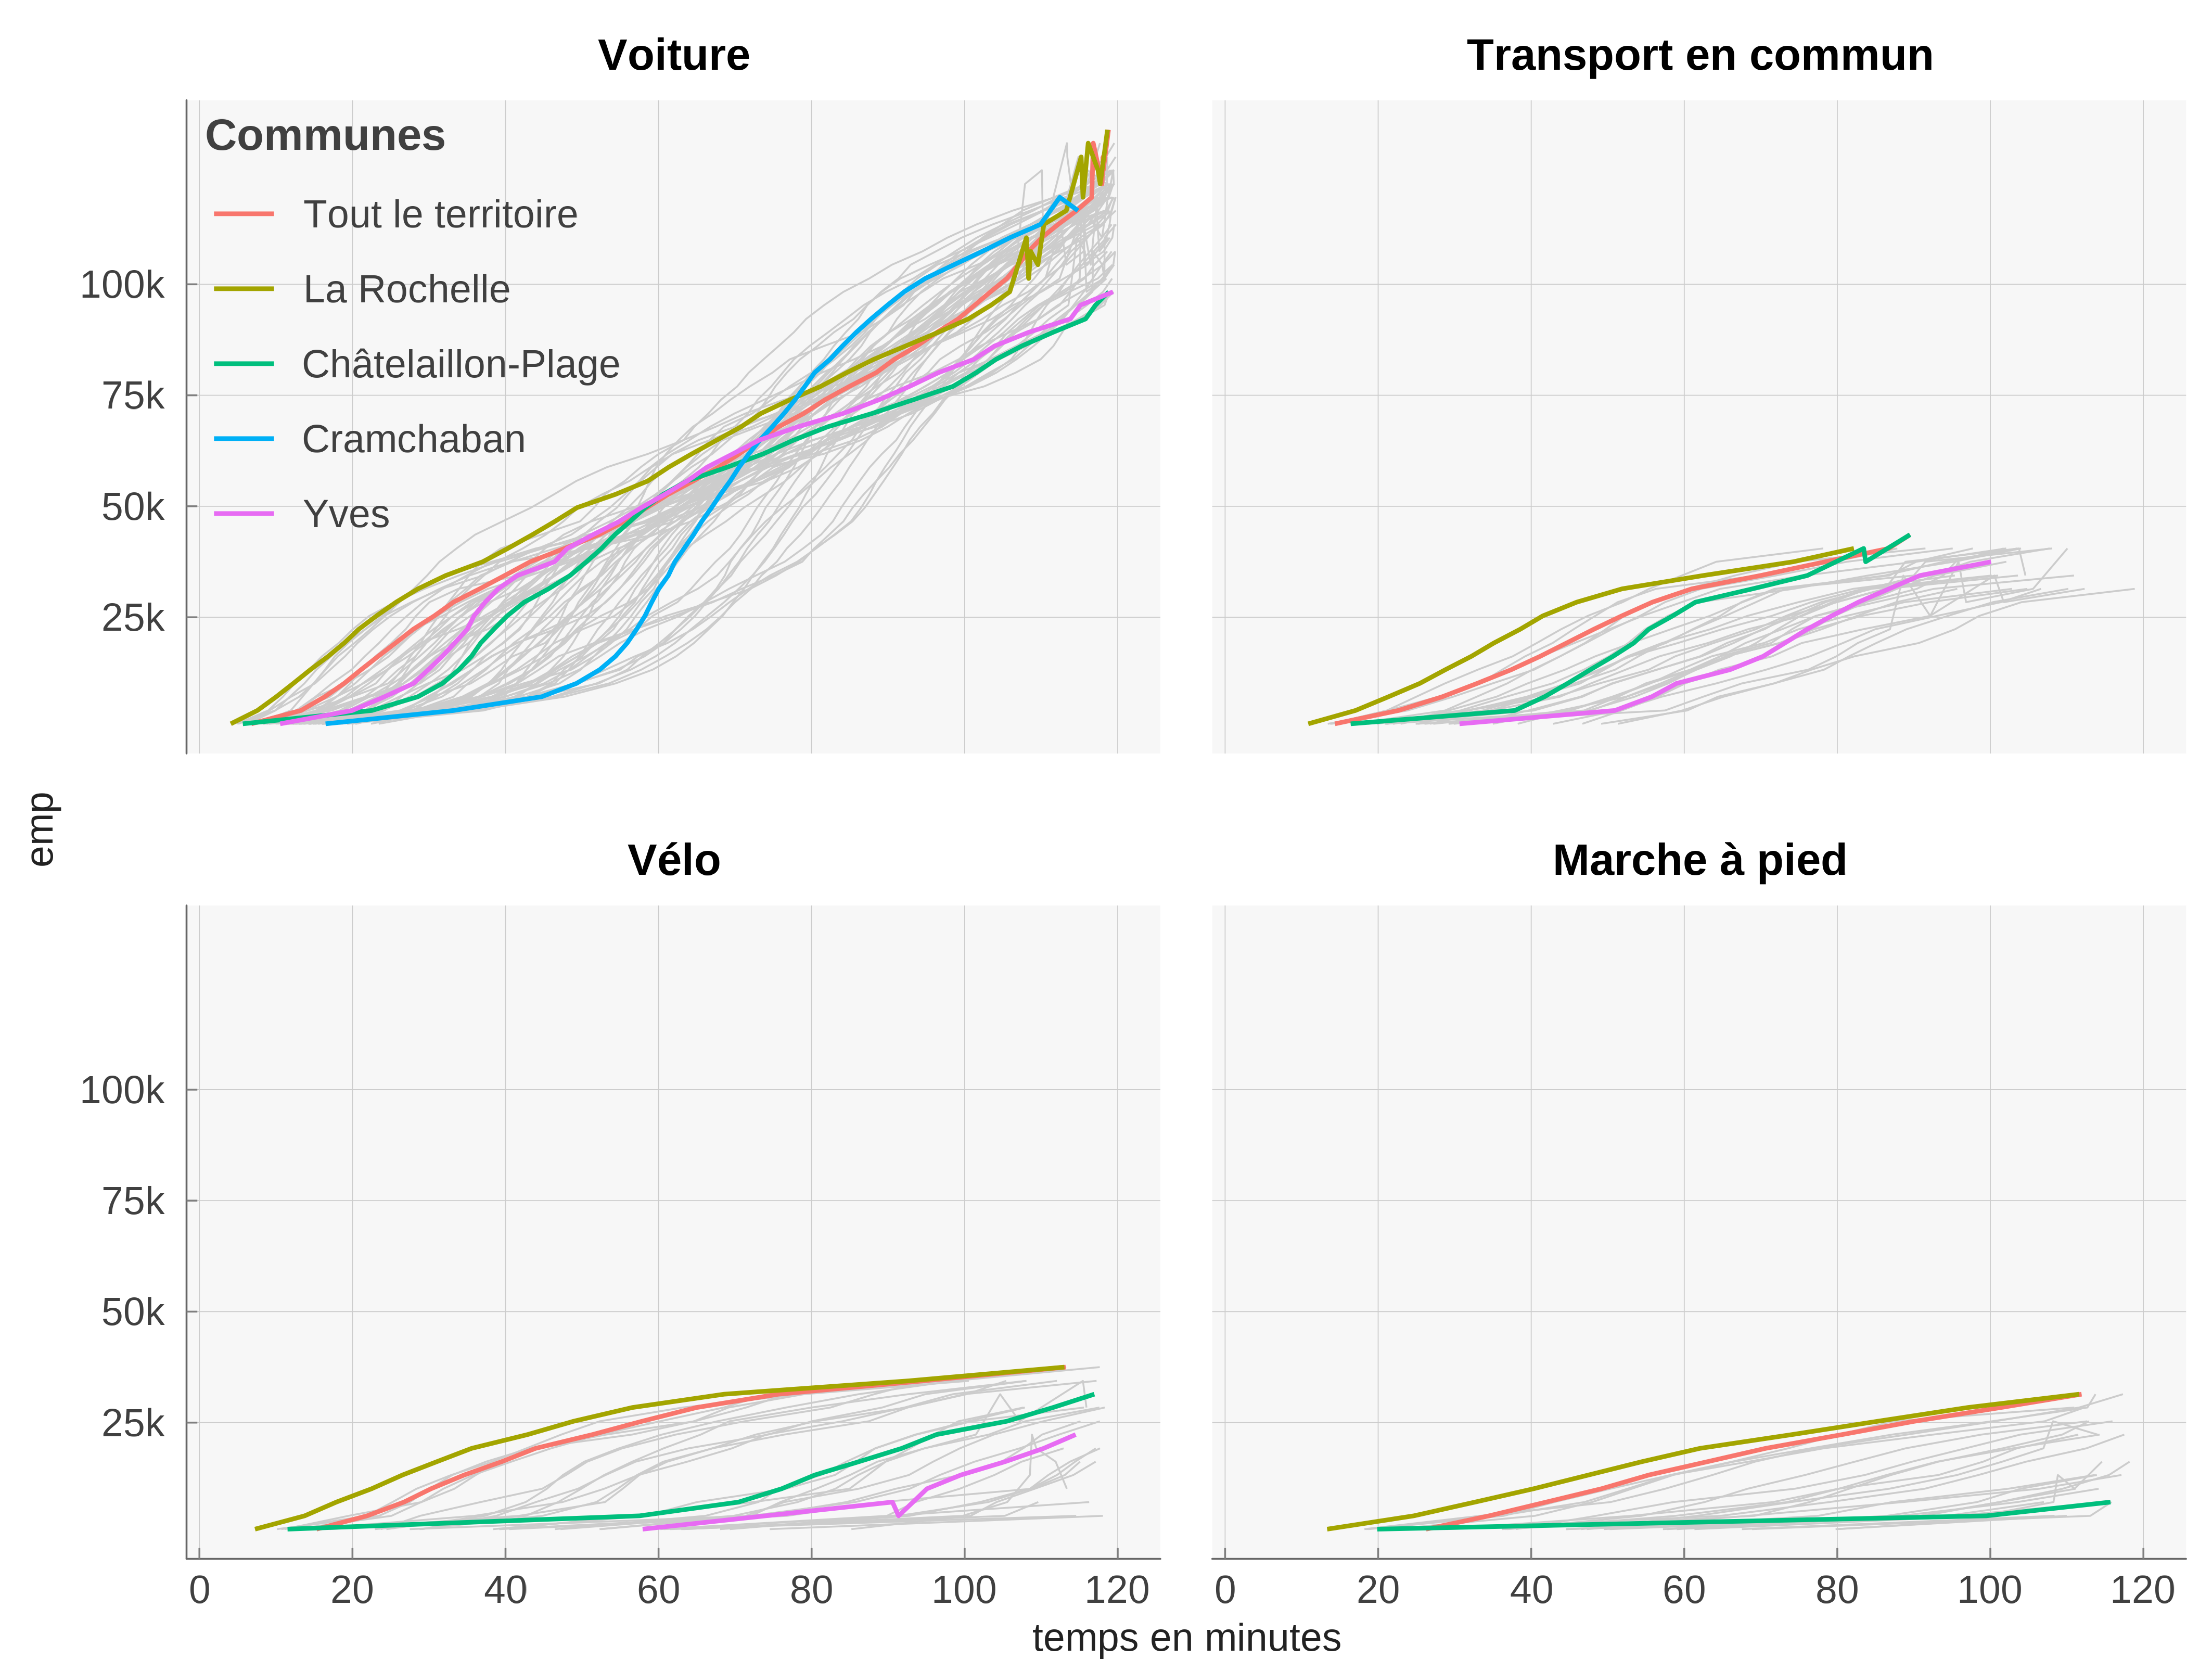
\includegraphics[width=1\textwidth,height=\textheight]{output/access_par_com.png}

}

\caption[Accessibilité par communes pour la
Rochelle]{\label{fig-comaccess}Courbe du temps d'accès aux emplois. Pour
chaque commune, on calcule la médianne, pondérée par le nombre
d'habitants par carreau, du temps d'accès à différents seuils d'emplois.
Cela permet de caractériser les communes par leur accessibilité à
l'emploi, une mesure plus pertinente de la `distance à l'emploi'. Calcul
des auteurs. Sources : OSM, Mapbox, IGN, Conveyal R5, carroyage INSEE
2017, Flores et fichiers fonciers 2018}

\end{figure}

\hypertarget{ajustement-de-meaps-sur-mobpro}{%
\subsection{Ajustement de MEAPS sur
MOBPRO}\label{ajustement-de-meaps-sur-mobpro}}

La construction de la matrice de distance permet d'utiliser MEAPS pour
déduire les flux carreau à carreau. Mais le fichier détail du
recensement et son volet mobilités professionnelles nous donnent une
information supplémentaire que nous pouvons utiliser pour calibrer au
plus près des données MEAPS. Les mobilités professionnelles décrivent
pour chaque paire de commune résidence-emploi les flux de mobilités
professionnelles (de nombreuses paires de communes ont des flux nuls).
Cette information est équivalente à celle produite par MEAPS mais
agrégée au niveau communal. Une première stratégie de calage de MEAPS
est d'affecter aux probabilités d'absorption un facteur correcteur pour
reproduire le plus fidèlement possible les flux agrégés de INSEE
(2022a). Cette approche permet ensuite d'utiliser MEAPS sur les données
INSEE (2022a) pour réaliser une interpolation infra-communale des
déplacements, au carreau 200m. En accédant à ce niveau de détail, nous
pouvons ensuite mobiliser la méthode de calcul des distances et des
temps de trajets à une échelle fine pour produire des différences au
carreau 200m. Dans une autre approche, plus parcimonieuse, on pourrait
limiter le nombre de paramètres estimés pour MEAPS, afin d'une apprécier
la qualité prédictive et le comparer à une autre approche. Nous
détaillerons cette autre approche dans un futur document.

La modification des probabilités d'absorption est faite par l'ajout d'un
facteur correcteur exprimé en ``chance'', c'est-à-dire que la
probabilité modifiée l'est par la formule suivante où \(\omicron_{i,j}\)
est un nombre entre \(0\) et \(+\infty\) et \(i,j\) indexent les
communes de départ et d'arrivée avec \(c_a = p_a/(1-p_a)\):

\begin{equation}\protect\hypertarget{eq-odd}{}{
\tilde{p}_a = \frac{c_a \times \omicron_{i,j}} {1+c_a \times \omicron_{i,j}} 
}\label{eq-odd}\end{equation}

A ce stade nous utilisons un algorithme naïf pour trouver une solution
au problème posé. Nous calculons l'\emph{odd-ratio} entre le résultat
d'une simulation associée à un ensemble d'\(\omicron_{i,j}\) et celui
défini par les données observées de INSEE (2022a) en utilisant la
formule suivante où \(\beta\) est un paramètre d'amortissement inférieur
à 1 et positif et \(k\) indexe les itérations :

\begin{equation}\protect\hypertarget{eq-algest}{}{
\omicron^k_{i,j} = (\frac{\tilde{p}^k_a/(1-\tilde{p}^k_a)}{
p^{mobpro}_a/(1-p^{mobpro}_a)})^\beta \times \omicron^{k-1}_{i,j}
}\label{eq-algest}\end{equation}

Nous modifions alors les \(\omicron_{i,j}\) en fonction des écarts
observés. Cela conduit à chercher un point fixe. Nous calculons ensuite
un critère d'ajustement à partir de l'entropie relative de
Kullback-Leibler (Kullback et Leibler 1951). L'entropie relative est
définie pour deux distributions de probabilités \(p\) et \(q\) comme
suit (dans le cas discret, le cas continu se généralise aisément) :

\begin{equation}\protect\hypertarget{eq-kl}{}{
KL(p,q) = \sum_{i}p_i \times log(p_i/q_i)
}\label{eq-kl}\end{equation}

Cette mesure ressemble à une distance, mais n'est pas symétrique et ne
vérifie pas l'inégalité triangulaire. Elle s'interprète dans le cadre de
la théorie de l'information comme la quantité relative d'information
supplémentaire nécessaire pour exprimer \(q\) à partir de \(p\). En
suivant Colin Cameron et Windmeijer (1997) on peut construire un
coefficient \(R_{KL}^2\) de la façon suivante, où \(\hat{q}\) et \(q_0\)
sont deux distributions respectivement estimée et de référence que l'on
compare à \(p\) :

\begin{equation}\protect\hypertarget{eq-r2kl}{}{
R_{KL}^2 = 1 - \frac{KL(p,\hat{q})}{KL(p, q_0)}
}\label{eq-r2kl}\end{equation}

La distribution de référence est choisie comme une distribution
uniforme, par analogie avec le calcul de la variance dans un \(R^2\)
habituel où l'on régresse sur une constante. On écrit :

\begin{equation}\protect\hypertarget{eq-klent}{}{
\begin{aligned}
KL(p,q_{ref}) &{}= \sum_{i}p_i \times log(p_i/unif) \\&{}= \sum_i p_i \times log(p_i) + log(N)
\end{aligned}
}\label{eq-klent}\end{equation}

qui n'est autre que l'entropie de la distribution \(p\) à une constante
près (\(N\) est le nombre de résidents actifs ou d'emplois).

L'algorithme employé devra être affiné dans le futur afin de permettre
une descente de gradient qui permet de minimiser l'entropie relative.
L'algorithme naïf permet de réduire cette entropie relative sans assurer
qu'elle est minimale. Nous utiliserons l'algorithme naïf pour explorer
la possibilité d'ajuster MEAPS sur un jeu de données. Cet algorithme a
été utilisé avec différentes contraintes sur les paramètres. Le
tableau~\ref{tbl-meapsR2} indique la qualité de l'ajustement obtenu dans
ces différentes configurations. La première est celle où les
probabilités d'absorption sont déterminées uniquement par les fuites par
commune de résidence. C'est la configuration la plus parcimonieuse en
termes de paramètres et qui sert de référence. Le \(R^2_{KL}\) vaut
89.1\% ce qui est déjà un ajustement élevé. La seconde configuration est
celle où l'on ajuste des \(\omicron_{i,j}\) uniquement pour les termes
diagonaux (\(i=j\)). Cette configuration ajuste donc un \emph{odd-ratio}
pour les résidents qui travaillent dans leur commune de résidence. Dans
un certain nombre de communes, cet ajustement conduit à augmenter la
probabilité d'absorption interne (figure~\ref{fig-carteodd}), ce qui
indique que le choix de résidence n'est pas indépendant de celui
d'activité. Pour la commune la plus importante (la Rochelle), en
revanche, l'\emph{odd-ratio} \(\omicron_{17300, 17300}\) est proche de
1. Les deux configurations suivantes laissent beaucoup plus de degrés de
liberté en estimant des \(\omicron_{i,j}\) librement. La première de ces
deux configurations limite les \(\omicron_{i,j}\) estimés à ceux
représentant un total cumulé des flux mesurés par INSEE (2022a) égal à
98\% ce qui représente un peu moins de 2 000 \(\omicron_{i,j}\). La
seconde configuration estime tous les \(\omicron_{i,j}\) sans limite
(soit 15 120 paramètres pour 72 communes de résidence et 210 communes
d'activité).

\hypertarget{tbl-meapsR2}{}
\setlength{\LTpost}{0mm}
\begin{longtable}{lrrr}
\caption{\label{tbl-meapsR2}Ajustement de MEAPS }\tabularnewline

\toprule
 & N(pf,i) & N(oi,j) & RKL2 \\ 
\midrule
Fuite par commune de résidence & $72$ & $0$ & $89.1\%$ \\ 
Fuite et diagonale & $72$ & $72$ & $94.3\%$ \\ 
Fuite et 90\% des flux & $72$ & $729$ & $95.9\%$ \\ 
Fuite et 99\% des flux & $72$ & $1 928$ & $98.3\%$ \\ 
Fuite et 100\% des flux & $72$ & $15 120$ & $99.0\%$ \\ 
\bottomrule
\end{longtable}
\begin{minipage}{\linewidth}
L\textquotesingle{}ajustement de MEAPS est réalisé par l\textquotesingle{}algorithme décrit dans le texte. Le nombre de paramètres estimés est égal à la somme de la colonne N(pf,i) et de la colonne N(oi,j).\\
\end{minipage}

la figure~\ref{fig-actvsfit} représente les flux observés et estimés
pour les différentes configurations du tableau~\ref{tbl-meapsR2}. Le
gain à estimer les \(\omicron_{i,i}\) diagonaux, pondérant les flux
allant d'une commune de résidence vers elle même est assez élevé,
faisant passer le \(R^2_{KL}\) de 89.1\% à 94.3\% et réduisant les
écarts entre flux observé et flux estimé comme le montrent les deux
panneaux supérieurs de la figure~\ref{fig-actvsfit}. L'ajout de
paramètres supplémentaires ne fait pas gagner beaucoup plus d'autant que
les écarts pour les flux marginaux ne sont pas tant réduit que ça. La
limite de l'algorithme naïf apparaît ici, puisque le modèle complètement
saturé n'ajuste pas totalement la distribution. Différents détails de
l'algorithme peuvent l'expliquer, notamment la censure des
\emph{odd-ratio} trop faibles (\textless0.001) ou trop importants
(\textgreater1000). Au-delà de cet argument, il est probable que pour
converger vers un ajustement plus strict, il serait nécessaire de
calculer la matrice des quasi dérivées des flux par rapport aux
\(\omicron_{i,j}\).

Mais le coût peut être très élevé puisque cette matrice (calculée dans
la partie synthétique dans un cas simple) est d'une taille considérable
(15 120 \(\times\) 15 120 coefficients), surtout si l'on prend en compte
que le calcul de chaque terme prend quelques dizaine de
secondes\footnote{Autour de mille années de vCPU\ldots{}}.

\begin{figure}[htb]

{\centering 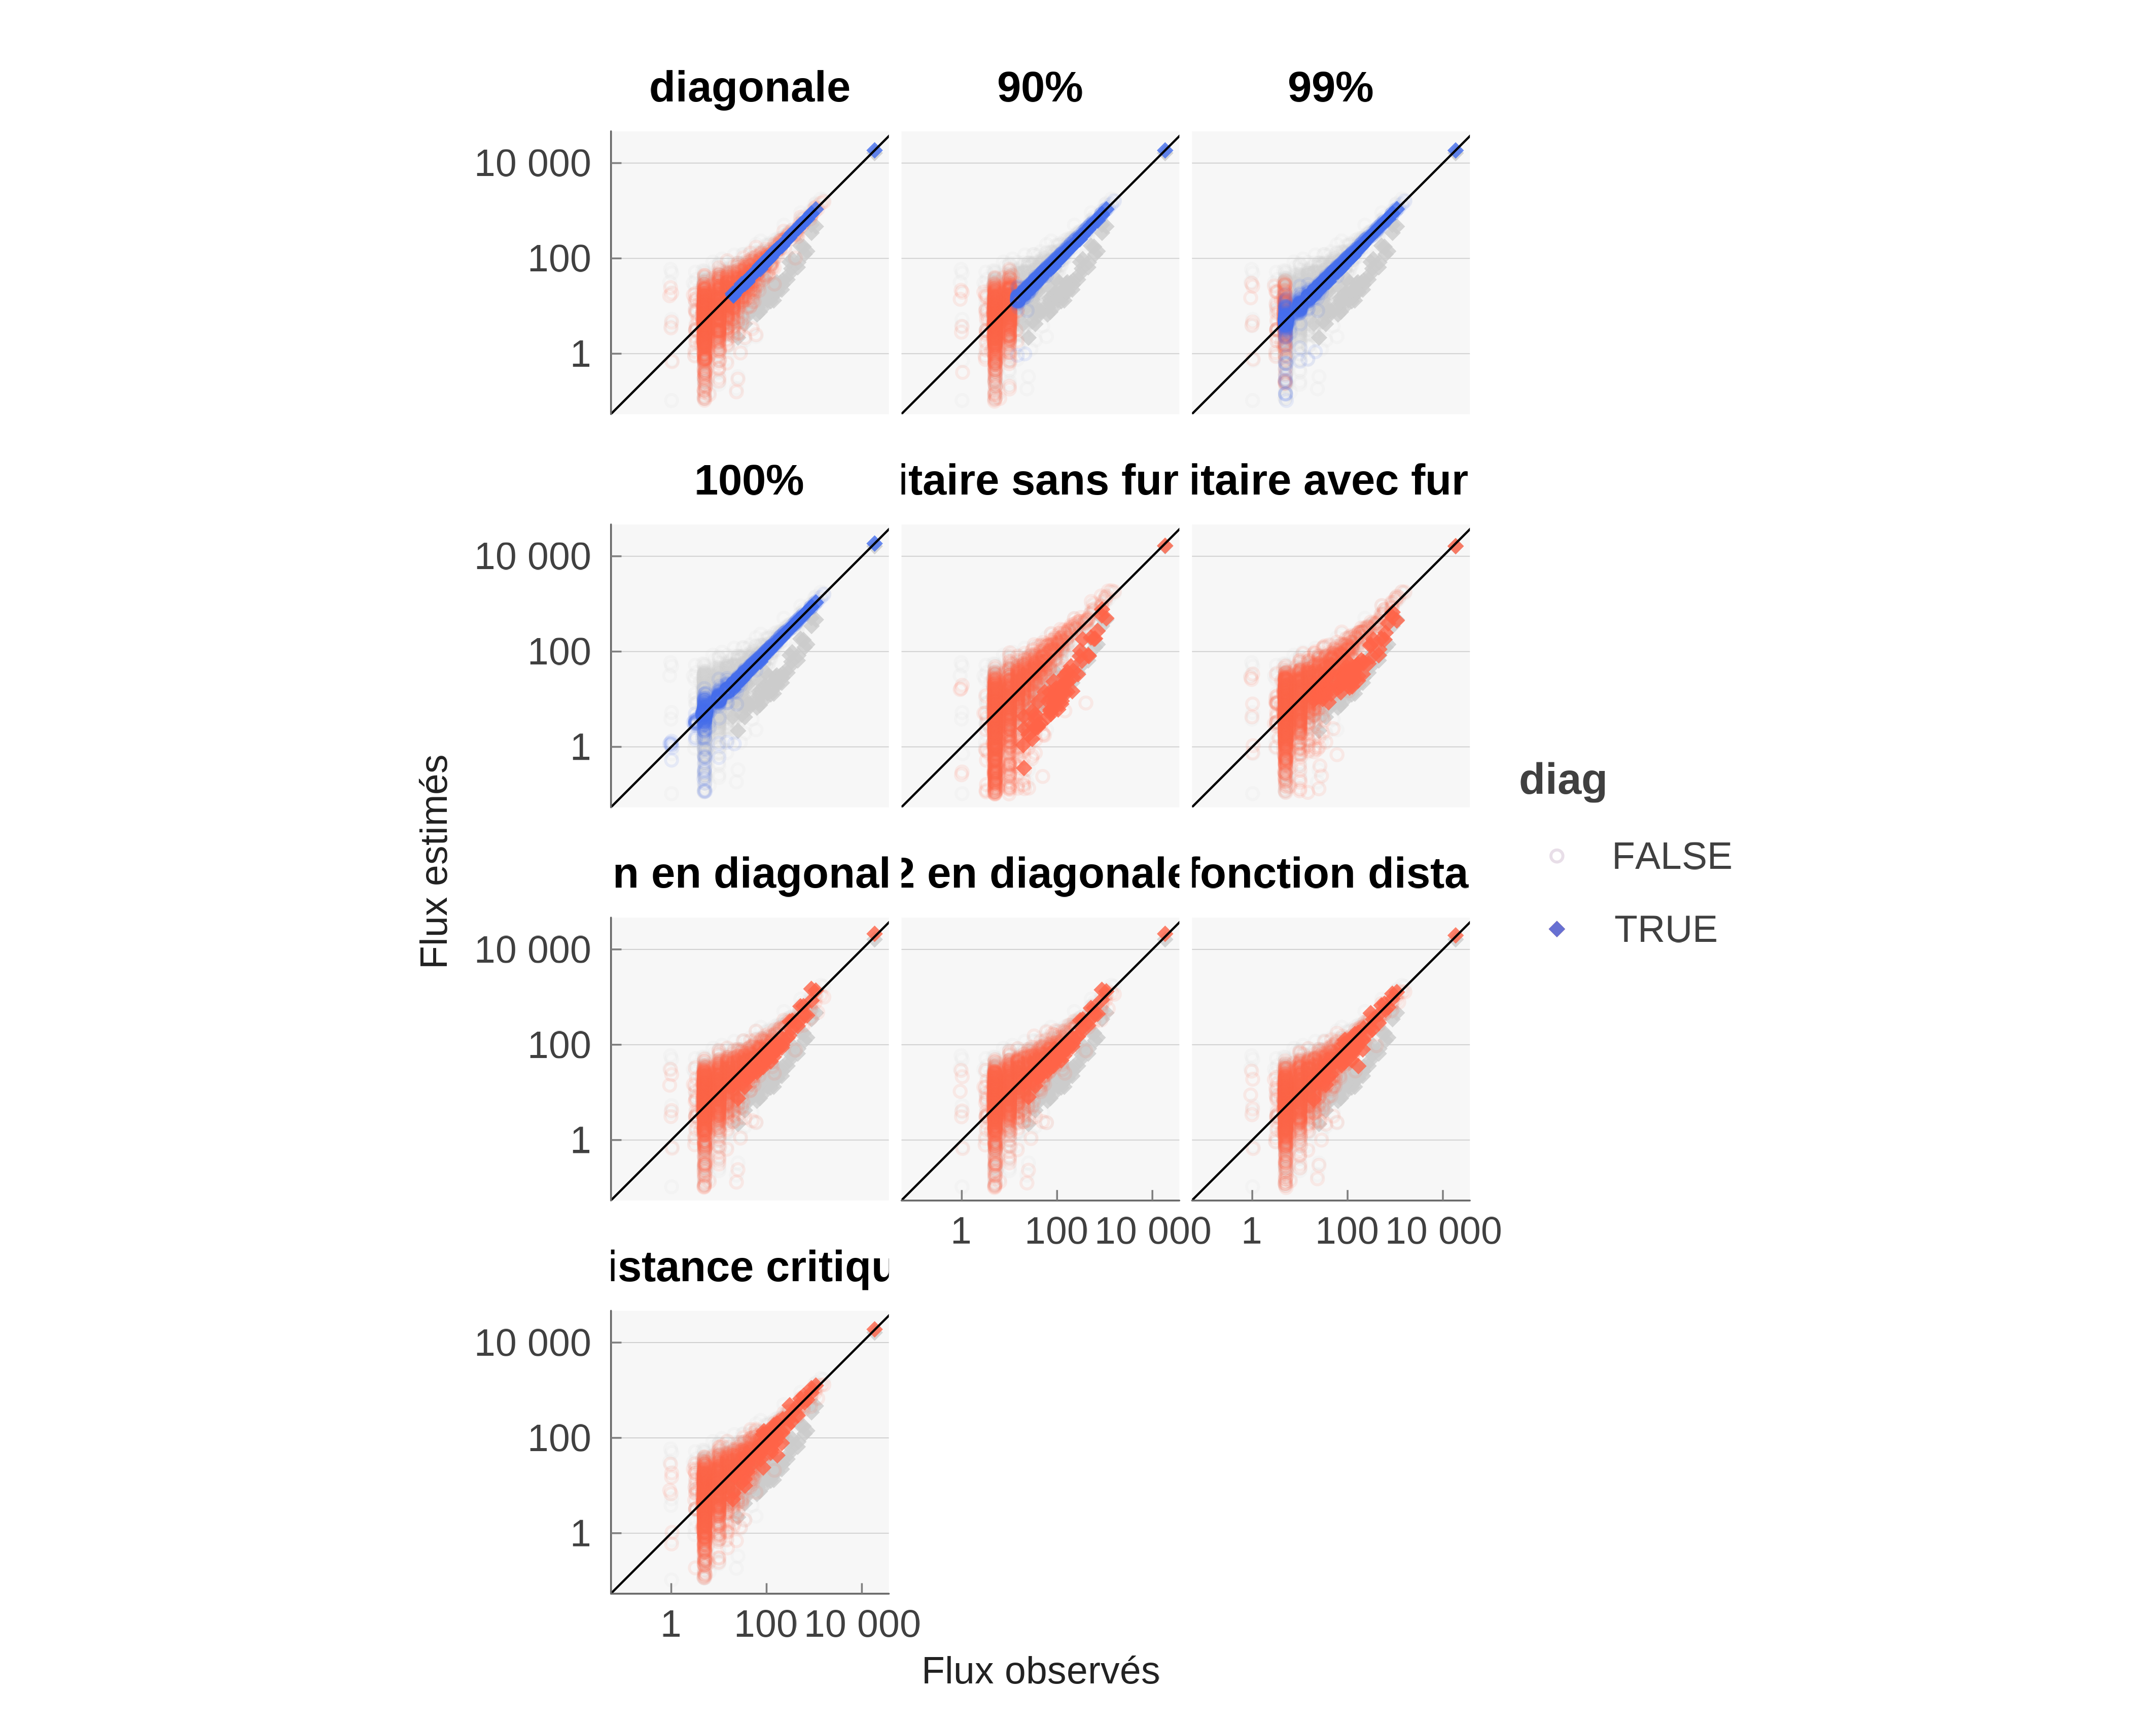
\includegraphics[width=1\textwidth,height=\textheight]{output/estmeaps.png}

}

\caption[MEAPS observés versus estimés]{\label{fig-actvsfit}La figure
présente pour chaque configuration d'estimation le flux observé (axe des
x) et le flux estimé (axe des y) en bleu lorsque oi,j est estimé et en
vert lorsqu'il n'est pas estimé. La valeur de référence est répétée dans
chaque panneau en gris clair.}

\end{figure}

Pour les 20 plus grandes communes de l'agglomération de la Rochelle --
qui comptent plus de 1 000 résidents en activité -- on peut représenter
les \emph{odd-ratios} estimés (dans la configuration 100\% des flux) en
fonction de la distance de la commune de destination à la commune de
résidence. L'élément le plus frappant est que les odd-ratios de \(i\) à
\(i\) sont généralement supérieur à 1, à l'exception de la commune de la
Rochelle. Il n'émerge pas de structure particulière par rapport à la
distance, si ce n'est des \emph{odd-ratios} élevés pour des distances
importantes.

\begin{figure}[htb]

{\centering 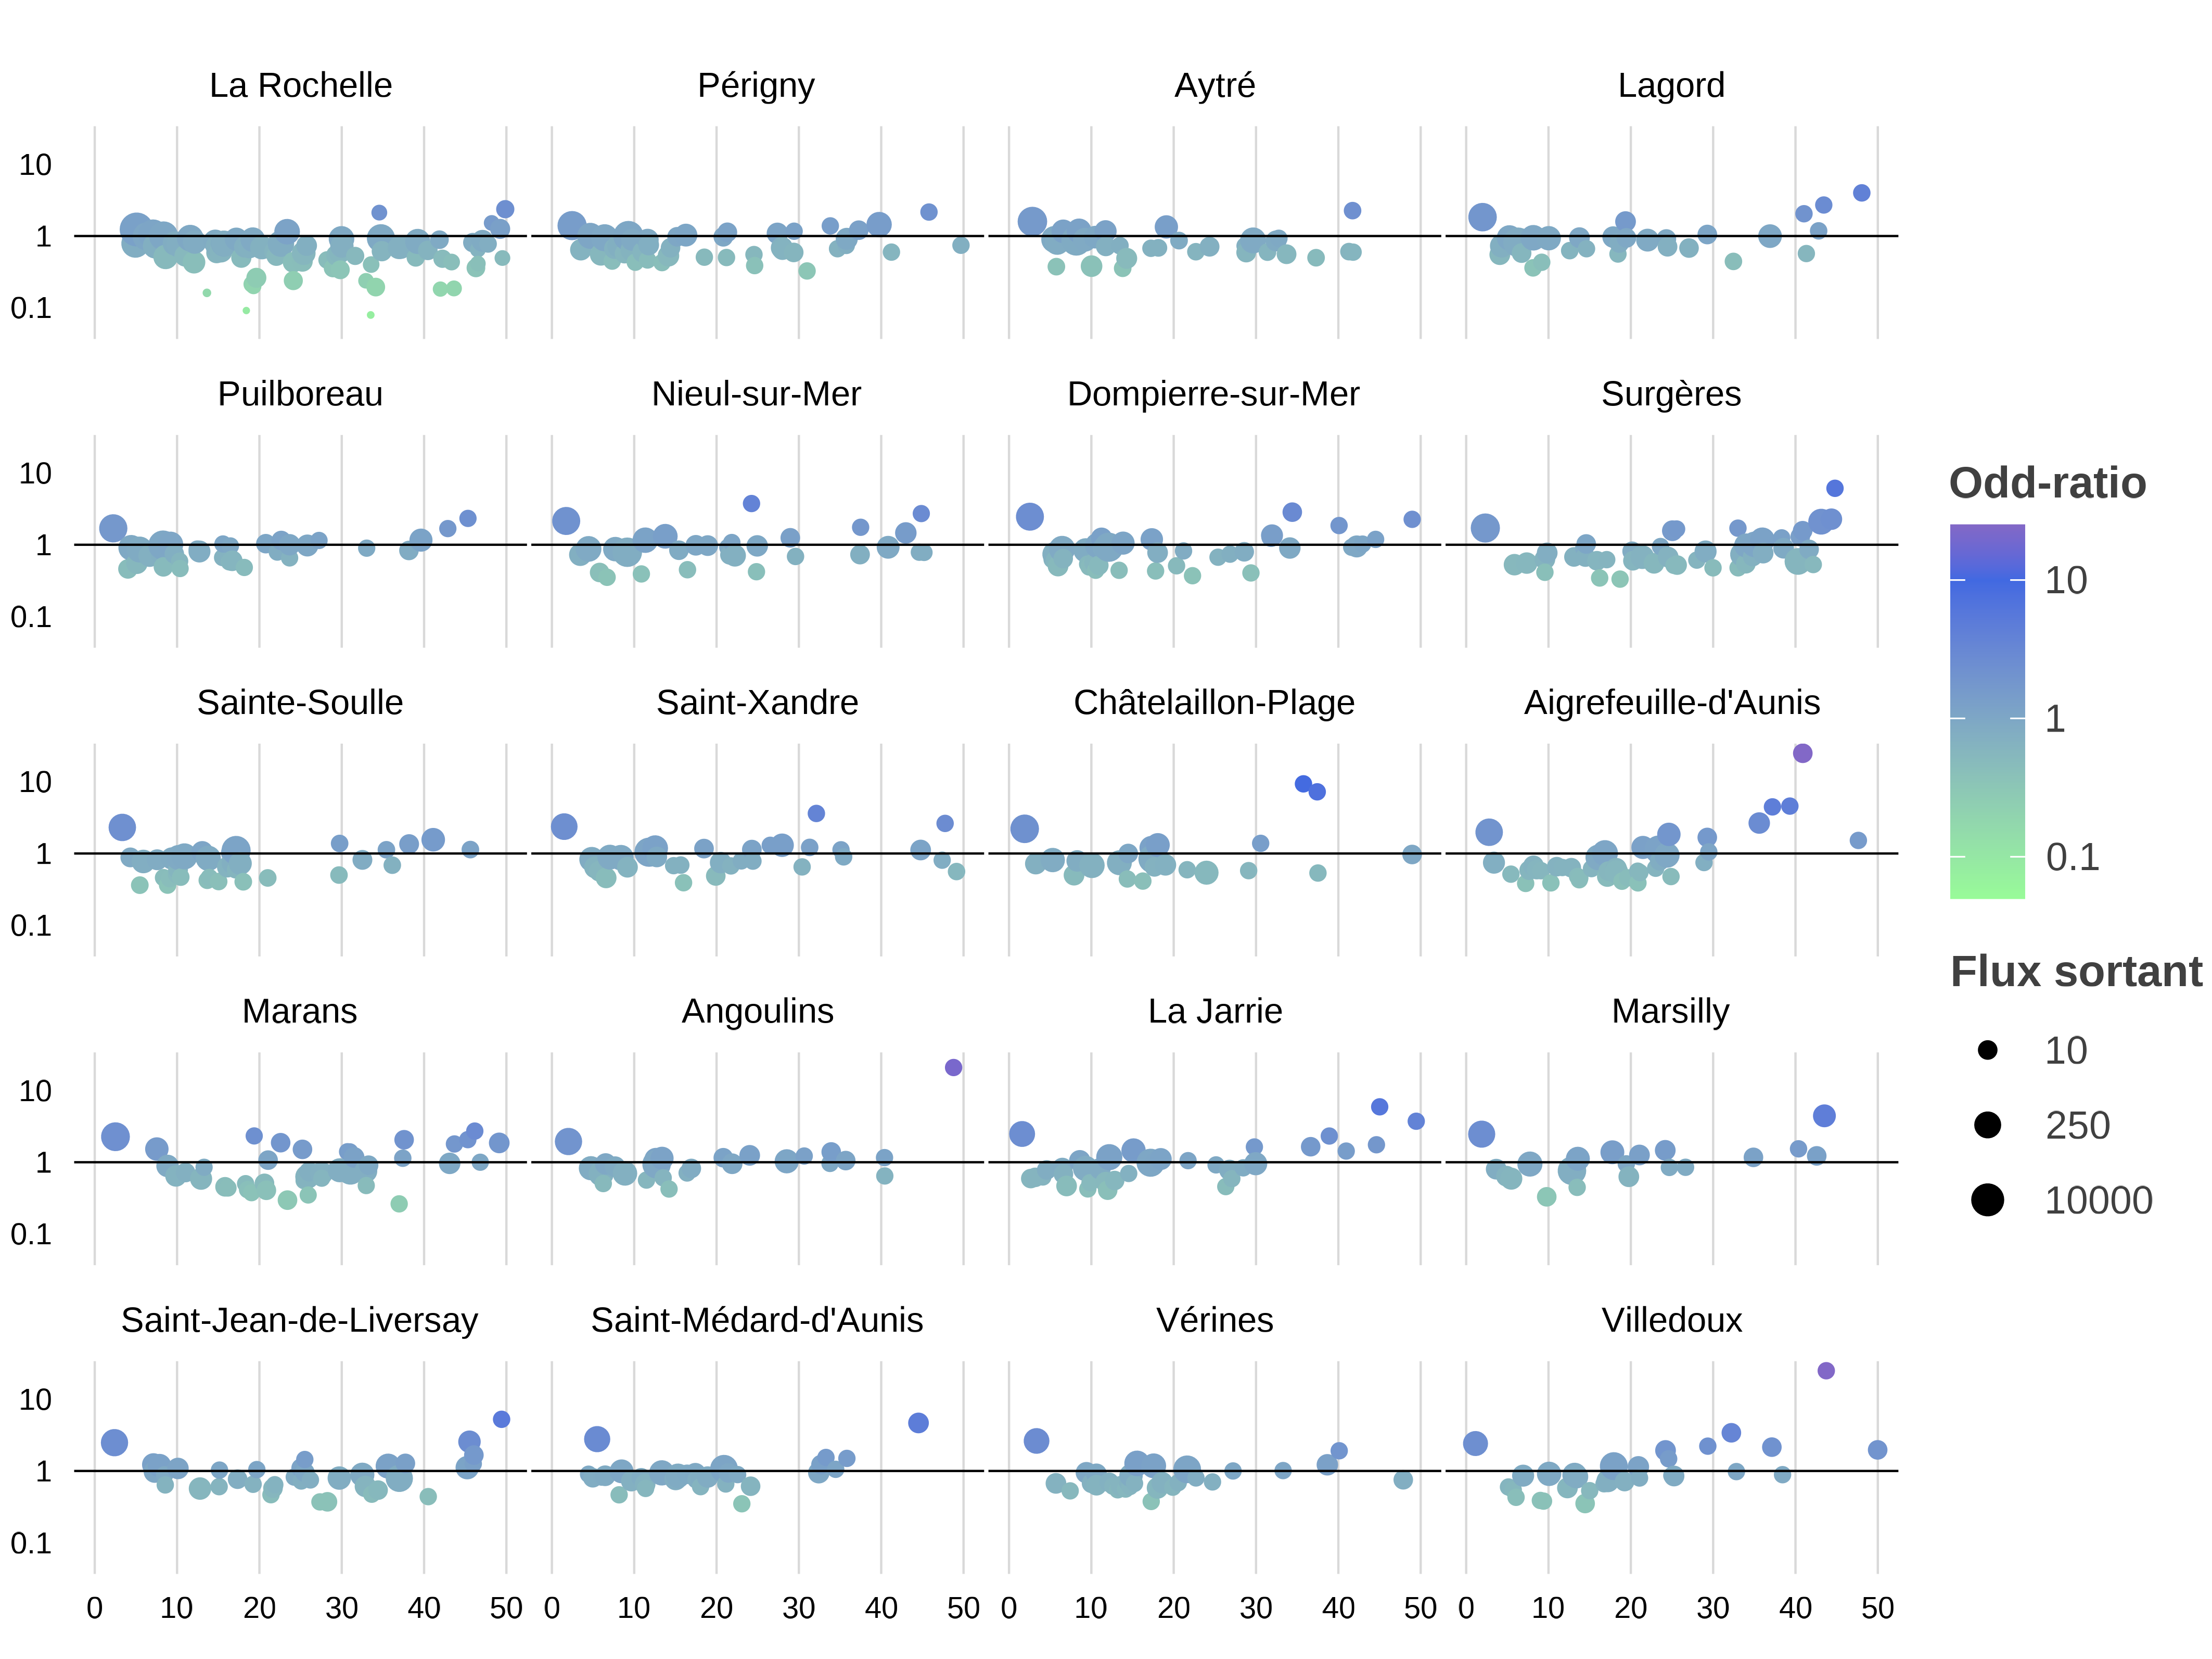
\includegraphics[width=1\textwidth,height=\textheight]{output/spectre100.png}

}

\caption[Odd-ratio en fonction de la distance
(spectre)]{\label{fig-spectre}La figure représente pour les 20 plus
grandes communes de l'agglomération de la Rochelle les odd-ratios
estimés (100\% des flux) en fonction de la distance entre commune. La
distance est construite comme la distance moyenne pondérée entre les
résidents de la commune de départ et les emplois de la commune
d'arrivée. La pondération est le produit des emplois et des résidents
pour chqeu paire, normalisé à 1.}

\end{figure}

La carte de la figure~\ref{fig-carteodd} permet de préciser la valeur
élevée des \emph{odd-ratio} pour les flux internes. Les communes où sont
localisés de nombreux emplois ont un \emph{odd-ratio} plutôt plus faible
alors qu'ils sont estimés plus élevés dans les communes plus petites et
moins desservies. Un \emph{odd-ratio} élevé indique que les flux
internes sont plus élevés que dans le scénario de référence {[}{[}ce
serait bien de calculer les probabilités d'absorption (qui dépendent des
fuites et de tous les \emph{odds} plutôt que de discuter des
odds){]}{]}. Cela indique probablement un choix de résidence en lien
avec l'emploi occupé en privilégiant la commune d'activité pour la
résidence (ou l'inverse). Le spectre en fonction de la distance indique
que ce phénomène, s'il est un hypothèse à très faible distance, ne
persiste pas en dehors de la commune de résidence.\\

\begin{figure}[htb]

{\centering \includegraphics[width=1\textwidth,height=\textheight]{output/diagonale.png}

}

\caption[Odd-ratio dans la diagonale]{\label{fig-carteodd}Chaque cercle
indique les odd-ratio estimés dans la diagonale (100\% des flux). Les
diamètres des cercles sont proportionels aux flux internes (de i à i).}

\end{figure}

\hypertarget{scuxe9narios-localisation-de-lemploi}{%
\subsection{Scénarios ``localisation de
l'emploi''}\label{scuxe9narios-localisation-de-lemploi}}

Le Schéma de Cohérence Territorial (SCoT) est un document de
planification, établi et voté par les élus des communes composant le
territoire et soumis à validation de l'État. Il défini, entre autres,
des zones de développement économique, urbaines et des espaces naturels.
C'est la loi SRU relative à la Solidarité et au Renouvellement Urbains
du 13 décembre 2000 qui l'a défini et les contours en ont été modifiés
au cours des dernières années.

Le schéma n'est pas qu'indicatif puisqu'il est opposable. En ce qui
concerne le développement de l'emploi, la création de zones d'activité
est rendue possible par le SCoT, mais la réalisation effective des
créations d'emploi et surtout leur localisation nette des déplacements
d'autres emplois découle des décisions de l'ensemble des acteurs et donc
et donc de causalités diverses et variées. Nous évaluons ici des
scénarios comptatible avec le SCoT sans pour autant nous prononcer quant
à leur réalisme ou leur probabilité d'occurrence. Ainsi, nous analysons
les localisations proposées à emploi total constant, c'est-à-dire vues
comme des relocalisations de l'emploi vers les zones d'activités depuis
leur localisation actuelle.

La construction de cette analyse impose donc de connaître précisément la
localisation de l'emploi, ce que nous réalisons par une imputation au
carreau INSPIRE 200m à partir des données d'emploi par
commune{[}\^{}16{]}. Nous calons alors MEAPS sur ces données ainsi que
sur les données de mobilité professionnelles issues du
recensement\footnote{https://www.insee.fr/fr/information/2383243} et
publiées par l'INSEE. Ces données donnent les lieux habituels de travail
(à la commune) pour les différents résidents (d'une commune) ainsi que
les flux correspondant entre paires de communes.

La construction de cette analyse impose donc de connaître précisément la
localisation de l'emploi, ce que nous réalisons par une imputation au
carreau INSPIRE 200m à partir des données d'emploi par commune. Nous
calons alors MEAPS sur ces données ainsi que sur les données de mobilité
professionnelles issues du recensement\footnote{Autour de mille années
  de vCPU\ldots{}} et publiées par l'INSEE. Ces données donnent les
lieux habituels de travail (à la commune) pour les différents résidents
(d'une commune) ainsi que les flux correspondant entre paires de
communes.

\begin{itemize}
\tightlist
\item
  Une fois MEAPS calé sur ces données, nous pouvons analyser des
  scénarios de déplacement des emplois et en déduire les conséquences en
  trajets, mode de transport et donc émissions de CO\textsubscript{2}
  associé
\end{itemize}

\hypertarget{scuxe9narios-transport-en-commun}{%
\subsection{Scénarios ``transport en
commun''}\label{scuxe9narios-transport-en-commun}}

L'analyse du territoire ne repose pas seulement sur la localisation de
l'emploi, mais aussi sur une prise en compte détaillée des possibilités
de transport.

\newpage{}

\hypertarget{bibliographie}{%
\section*{Bibliographie}\label{bibliographie}}
\addcontentsline{toc}{section}{Bibliographie}

\hypertarget{refs}{}
\begin{CSLReferences}{1}{0}
\leavevmode\vadjust pre{\hypertarget{ref-ben-akiva2018}{}}%
Ben-Akiva, Moshe, et Steven R. Lerman. 2018. \emph{Discrete Choice
Analysis: Theory and Application to Travel Demand}. Transportation
Series. MIT Press.

\leavevmode\vadjust pre{\hypertarget{ref-colincameron1997}{}}%
Colin Cameron, A., et Frank A. G. Windmeijer. 1997. {«~An R-Squared
Measure of Goodness of Fit for Some Common Nonlinear Regression
Models~»}. \emph{Journal of Econometrics} 77 (2): 329‑42.
\url{https://doi.org/10.1016/s0304-4076(96)01818-0}.

\leavevmode\vadjust pre{\hypertarget{ref-conway2017}{}}%
Conway, Matthew Wigginton, Andrew Byrd, et Marco van der Linden. 2017.
{«~Evidence-Based Transit and Land Use Sketch Planning Using Interactive
Accessibility Methods on Combined Schedule and Headway-Based
Networks~»}. \emph{Transportation Research Record: Journal of the
Transportation Research Board} 2653 (1): 45‑53.
\url{https://doi.org/10.3141/2653-06}.

\leavevmode\vadjust pre{\hypertarget{ref-conway2018}{}}%
Conway, Matthew Wigginton, Andrew Byrd, et Michael Van Eggermond. 2018.
{«~Accounting for uncertainty and variation in accessibility metrics for
public transport sketch planning~»}. \emph{Journal of Transport and Land
Use} 11 (1). \url{https://doi.org/10.5198/jtlu.2018.1074}.

\leavevmode\vadjust pre{\hypertarget{ref-conway2019}{}}%
Conway, Matthew Wigginton, et Anson F. Stewart. 2019. {«~Getting Charlie
Off the MTA: A Multiobjective Optimization Method to Account for Cost
Constraints in Public Transit Accessibility Metrics~»}.
\emph{International Journal of Geographical Information Science} 33 (9):
1759‑87. \url{https://doi.org/10.1080/13658816.2019.1605075}.

\leavevmode\vadjust pre{\hypertarget{ref-de2011modelling}{}}%
Dios Ortúzar, Juan de, et Luis G Willumsen. 2011. \emph{Modelling
transport}. John wiley \& sons.

\leavevmode\vadjust pre{\hypertarget{ref-heanue1966}{}}%
Heanue, Kevin E., et Clyde E. Pyers. 1966. {«~A Comparative Evaluation
of Trip Distribution Procedures~»}. \emph{Highway Reserach Record}, nᵒ
114: 20‑50.

\leavevmode\vadjust pre{\hypertarget{ref-handbook2007}{}}%
Hensher, David A., et Kenneth J. Button, éd. 2007. {«~Handbook of
Transport Modelling~»}. \emph{Handbooks in Transport}, septembre.
\url{https://doi.org/10.1108/9780857245670}.

\leavevmode\vadjust pre{\hypertarget{ref-MOBPRO}{}}%
INSEE. 2022a. {«~Mobilités professionnelles en 2019 : déplacements
domicile - lieu de travail Recensement de la population - Base flux de
mobilité~»}. \url{https://www.insee.fr/fr/statistiques/6454112}.

\leavevmode\vadjust pre{\hypertarget{ref-C200}{}}%
---------. 2022b. {«~Revenus, pauvreté et niveau de vie en 2017 -
Données carroyées. Dispositif Fichier localisé social et fiscal
(Filosofi)~»}.
\url{https://www.insee.fr/fr/statistiques/6214811?sommaire=6215217}.

\leavevmode\vadjust pre{\hypertarget{ref-kullback1951}{}}%
Kullback, S., et R. A. Leibler. 1951. {«~On Information and
Sufficiency~»}. \emph{The Annals of Mathematical Statistics} 22 (1):
79‑86. \url{https://doi.org/10.1214/aoms/1177729694}.

\leavevmode\vadjust pre{\hypertarget{ref-lasser2020}{}}%
Lasser, Jana. 2020. {«~Creating an Executable Paper Is a Journey Through
Open Science~»}. \emph{Communications Physics} 3 (1).
\url{https://doi.org/10.1038/s42005-020-00403-4}.

\leavevmode\vadjust pre{\hypertarget{ref-OpenStreetMap}{}}%
OpenStreetMap contributors. 2017. {«~{Planet dump retrieved from
https://planet.osm.org}~»}. \url{https://www.openstreetmap.org}.

\leavevmode\vadjust pre{\hypertarget{ref-patrickbonnel2001}{}}%
Patrick Bonnel. 2001. {«~Prévision de la demande de transport~»}. Thèse
de doctorat, Lyon, France.

\leavevmode\vadjust pre{\hypertarget{ref-r5r}{}}%
Rafael H. M. Pereira, Marcus Saraiva, Daniel Herszenhut, Carlos Kaue
Vieira Braga, et Matthew Wigginton Conway. 2021. {«~r5r: Rapid Realistic
Routing on Multimodal Transport Networks with R5 in R~»}.
\url{https://doi.org/10.32866/001c.21262}.

\leavevmode\vadjust pre{\hypertarget{ref-MOBPERS}{}}%
SDES, Ministère de la transition écologique et de la cohésion des
territoires. 2021. {«~EMP 2019 Résultats détaillés de l'enquête mobilité
des personnes de 2019~»}.
\url{https://www.statistiques.developpement-durable.gouv.fr/resultats-detailles-de-lenquete-mobilite-des-personnes-de-2019}.

\leavevmode\vadjust pre{\hypertarget{ref-simini2012}{}}%
Simini, Filippo, Marta C. González, Amos Maritan, et Albert-László
Barabási. 2012. {«~A Universal Model for Mobility and Migration
Patterns~»}. \emph{Nature} 484 (7392): 96‑100.
\url{https://doi.org/10.1038/nature10856}.

\leavevmode\vadjust pre{\hypertarget{ref-stouffer1940}{}}%
Stouffer, Samuel A. 1940. {«~Intervening Opportunities: A Theory
Relating Mobility and Distance~»}. \emph{American Sociological Review} 5
(6): 845. \url{https://doi.org/10.2307/2084520}.

\leavevmode\vadjust pre{\hypertarget{ref-wilson1967}{}}%
Wilson, A. G. 1967. {«~A Statistical Theory of Spatial Distribution
Models~»}. \emph{Transportation Research} 1 (3): 253‑69.
\url{https://doi.org/10.1016/0041-1647(67)90035-4}.

\end{CSLReferences}

\newpage{}

\listoffigures

\listoftables



\end{document}
